\documentclass[fontsize=11pt, % size of the font
			   paper=a4,
			   chapterprefix=true,
			   % oneside, % other option: oneside
			   % chapterprefix=false, % specifies if the word chapter is printed for chapter headings
			   % BCOR=0mm, % offset for binding
			   setPDF, % sets twosided=semi, BCOR=0, DIV=classic if not specified
			   % showframe, % show the page layout
			   bibstyle=styleB,
			   ]{fau-math-thesis}
% ########################################################################################
% ########################################################################################
% Font encoding and font specification
% ----------------------------------------------------------------------------------------
\usepackage[T1]{fontenc}
\usepackage{lmodern}
% ########################################################################################
% The following specifies the titlepage and can not be deleted
% ----------------------------------------------------------------------------------------
\author{Martin Burger}
\semester{Sommersemester 2022}
\department{Department Mathematik, AMMN}
\title{Diskretisierung und numerische Optimierung}
%\date{Oct 01, 2021}
% ########################################################################################
\keywords{topicA, topicB, topicC} %keywords of your thesis
\setpdfinfo % For additional information in the pdf file
% ########################################################################################
% Bibliography
% ----------------------------------------------------------------------------------------
\addbibresource{backmatter/thesis-bibliography.bib}
% ########################################################################################
% Load the fau style packages with customization
% ----------------------------------------------------------------------------------------
% Color themes
\usepackage{styles/fau-colors}
\colorthemefaumath
% Appearence of boxes and page
\usepackage[thmboxing=styleA,
			boxingstyle=styleA,
			chapterheader=styleA, 
			footerheader=styleA,
			%noabbrev % no abbreviations in cleveref
			]{styles/fau-appearence}
% Command spec for symbols
\usepackage{styles/fau-symbols}
% ########################################################################################
% ########################################################################################
% ########################################################################################
% Custom commands and additional packages
% Put additional command definition below.
% Load additional packages below 
% ----------------------------------------------------------------------------------------
%
\usepackage{kantlipsum}
\usepackage[totoc]{idxlayout}
%
\begin{document}
%-------------------------------------------------
\frontmatter
%-------------------------------------------------
\maketitle
\tableofcontents
\listoffigures
%-------------------------------------------------
\mainmatter
%-------------------------------------------------
\chapter{Einleitung}

In dieser Vorlesung werden wir einige weiterführende Aspekte der numerischen Mathematik diskutieren, nämlich numerische Verfahren zur Lösung von Optimierungsproblemen und von (gewöhnlichen) Differentialgleichungen.
Optimierungsprobleme treten in irgendeiner Form in fast allen mathematischen Anwendungsbereichen auf, von klassischen ökonomischen Problemen über Materialoptimierung bis hin zu modernen Problemen in der Bildverarbeitung und im maschinellen Lernen. 
Methodisch knüpfen wir im Teil zur Optimierung an die iterativen Methoden zur Lösung von Gleichungssystemen an, allerdings kommen hier noch einige Aspekte dazu: Mit einem Optimierungsproblem im Hintergrund können wir die Iterationsverfahren anpassen um tatsächlich durch die Iteration die Funktionswerte zu verkleinern. 
Darüber hinaus werden wir geeignete Wahlen der Schrittweite kennenzulernen, um besser die Konvergenz gegen Minimierer oder zumindest stationäre Punkte gewährleisten zu können. 
Ein weiterer Aspekt ist die Optimierung unter Nebenbedingung und die Minimierung konvexer nichtdifferenzierbarer Probleme, die in vielen modernen Anwendungen auftreten. Dazu werden wir exemplarisch ein Verfahren kennenlernen.

Der weitere Teil der Vorlesung beschäftigt sich dann mit der Lösung von Differentialgleichungen, insbesonderen gewöhnlichen Differentialgleichungen.
Wir beginnen mit Anfangswertproblemen der Form
$$ u'(t) = F(u(t),t), \qquad u(0)=u_0, $$
die nur für spezielle Formen von $F$ gelöst werden können. 
Allgemeinere Funktionen $F:\R^n \rightarrow \R^n$ treten aber in einer Vielzahl von Anwendungen auf, z.B. bei den Newtonschen Gesetzen für die Dynamik von Teilchen. Die entstehenden Systeme sind dann auch beliebig gro{\ss}, z.B. in der Molekulardynamik, wo $u(t)$ die Koordinaten $M$ verschiedener Teilchen im Zeitverlauf beschreibt ($N=3M$). 
Andere klassische Anwendungsgebiete gewönlicher Differentialgleichungen sind die Populationsdynamik oder auch die Modellierung von Aktienmärkten, wo meist noch eine zufällige Komponente hinzugefügt wird (stochastische Differentialgleichungen). 
Die numerischen Verfahren zur Lösung von Anfangswertproblemen sind einerseits ähnlich zu Iterationsverfahren, wenn die Ableitung durch Differenzenquotienten auf einem Gitter approximiert wird, andererseits zu numerischer Integration, wenn man die äquivalente Formulierung als Volterra-Integralgleichung
$$ u(t) = u_0 + \int_0^t F(u(s),s)~ds$$
benutzt und Quadraturformeln auf das Integral anwendet. 
Ein wichtiger Aspekt ist dabei die Diskretisierung, d.h. wir müssen das unendlichdimensionale Problem der Differentialgleichung, in dem wir eine Funktion $u$ suchen, durch ein endlichdimensionales Problem approximieren, z.B. durch Werte auf einem Gitter. 
Mathematisch stellt sich dann natürlich die Frage ob und in welchem Sinne das diskretisierte Problem gegen das ursprüngliche konvergiert. 

Zum Abschluss werden wir auch Randwertprobleme betrachten, die zu partiellen Differentialgleichungen führen. Ein einfaches Beispiel ist die Lösung von
$$ - (a(x) u'(x))' + c(x) u(x) = f(x),  \quad x \in (0,1) $$
mit Randwerten $u(0)=u(1)=0$. 
Hier müssen wir die Diskretisierung auf einmal im ganzen Intervall $(0,1)$ durchführen und nicht von einem Schritt zum Nächsten wie bei Anfangswertproblemen. 
Die Diskretisierung liefert hier ein lineares Gleichungssystem, das wir anschlie{\ss}end lösen müssen. 
Die Abschätzung des Diskretisierungsfehlers erfordert dann weiterführende Methoden. 
\chapter{Numerische Lösung von Anfangswertproblemen} 

Im Folgenden wollen wir uns mit der numerischen Lösungen von Anfangswertproblemen für gewöhnliche Differentialgleichungen der Form

\begin{equation}
u'(t) = \frac{du}{dt} = F(t,u(t)), \quad u(0) = u_0 \label{eq:awp}
\end{equation}

beschäftigen, wobei $F: \mathbb{R}_+ \times \mathbb{R}^n \rightarrow \mathbb{R}^n$ eine gegebene stetige Funktion ist. Die Modellierung mit Differentialgleichungen ist oft kanonisch, da man nur verstehen muss wie sich eine Größe in hinreichend kleiner Zeit ändern wird, d.h. wir schreiben

\begin{equation*}
u(t+\Delta t)  \approx u(t) + \Delta t F(t,u(t)) ,
\end{equation*}

wobei der Unterschied zur Exaktheit in dieser Relation dann von höherer Ordnung in $\Delta t$ sein kann. Im Grenzwert $\Delta t \rightarrow 0$ erhalten wir dann die Differentialgleichungen.  Einfache Heuristiken für Differentialgleichungen kennen wir beispielsweise aus der Physik,

\begin{itemize}
\item Geschwindigkeit ist Änderung des Orts pro Zeit,
\item Beschleunigung ist Änderung der Geschwindigkeit pro Zeit,
\item Kraft ist Masse mal Beschleunigung.
\end{itemize}

Beschreibt $x(t)$ den Ort eines Teilchens zur Zeit $t$, $v(t)$ seine Geschwindigkeit und $a(t)$ die Beschleunigung, dann gilt

\begin{equation*}
v(t) = \frac{dx}{dt}(t), \quad a(t) =  \frac{dv}{dt}(t), \quad m a(t) = F(x(t),v(t),t),
\end{equation*}

wobei $F$ ein Kraftfeld ist. Diese Gesetze können wir auch als Differentialgleichungen für $x$ und $v$ (oder den Impuls $p(t)=m v(t)$) lesen, wenn wir $a$ eliminieren, es gilt dann
$$ \frac{d}{dt} (x(t),v(t)) = (v(t), F(x(t),v(t),t)). $$
Kennen wir den Anfangsort $x(0)$ und die Anfangsgeschwindigkeit $v(0)$, so haben wir ein Anfangswert für ein System von Differentialgleichungen (im $\mathbb{R}^3$ insgesamt sechs Gleichungen für sechs Unbekannte). 

In großen Systemen von $N$ Teilchen $x_1,\ldots,x_N$ hat man dann Gleichungen für jede Position und die Geschwindigkeiten $v_1,\ldots,v_N$, mit

\begin{equation*} 
\frac{d}{dt} (x_i(t),v_i(t))_{i=1,\ldots,N} = (v_i(t), F(x_1(t),v_1(t), \ldots x_N(t),v_N(t),t)).
\end{equation*}

Zur Beschreibung realer Vorgänge mit vielen Teilchen (Moleküle, Zellen, Tiere in Herden, Fußgänger, Autos ...) erhält man also schnell beliebig komplexe Systeme von Differentialgleichungen. Unser Ziel in diesem Kapitel ist es die numerische Lösung solcher Differentialgleichungen zu untersuchen, zuvor klären wir aber noch einige Grundlagen der gewöhnlichen Differentialgleichungen um diese auch vernünftig verstehen zu können.


\section{Theorie von Anfangswertproblemen für gewöhnliche Differentialgleichungen}

Wir diskutieren im Folgenden kurz einige theoretische Aspekte gewöhnlicher Differentialgleichungen. Wir beginnen mit einer allgemeinen Theorie der Existenz und Eindeutigkeit. Grundlage dafür ist eine Umformulierung in eine Fixpunktform, sodass wir dann einfach einen passenden Fixpunktsatz anwenden können. Ist $u \in C^1([0,T])$ eine Lösung des Anfangswertproblems \eqref{eq:awp}, dann gilt aus dem Hauptsatz der Integralrechnung auch
$$ u(t) = u_0 + \int_0^t F(s,u(s)) ~ds , \qquad 0 \leq s \leq T. $$
Dies können wir als Fixpunktgleichung $u= {\cal F}(u)$  in einem Banachraum interpretieren. Dafür können wir zwei Arten von Fixpunktsätzen anwenden: die erste Art (Satz von Browder, Schauder oder andere Varianten) basiert auf Kompaktheit, d.h. wenn man Funktionen $u$ in den Operator reinsteckt sind diese topologisch danach in einer schöneren Menge. Insbesondere hat diese Menge dann einen Fixpunkt. In unserem Fall entsteht die Kompaktheit aus dem Satz von Arzela--Ascoli, man kann zeigen, dass für $u_n$ beschränkt die Folge ${\cal F}(u_n)$ immer eine konvergente Teilfolge hat. Dies liefert den sogenannten Satz von Peano, der die Existenz einer Lösung für stetiges $F$ garantiert. Da man hier recht abstrakt und über Teilfolgen argumentiert, hat man keine Chance die Eindeutigkeit eines Fixpunkts nachzuweisen. 

Die zweite Art an Beweisen basiert eigentlich immer auf dem Banach'schen Fixpunktsatz, den wir hier näher diskutieren wollen. Dazu beachten wir, dass falls $F$ im zweiten Argument Lipschitz-stetig ist (mit Modul $L$), folgendes gilt 

\begin{align*} 
\Vert {\cal F}(u_1) - {\cal F}(u_2) \Vert_\infty &= \max_{0 \leq t \leq T} \vert \int_0^t F(s,u_1(s)) - F(s,u_2(s)) ~ds \vert \\
&\leq  \max_{0 \leq t \leq T} \int_0^t \vert  F(s,u_1(s)) - F(s,u_2(s))\vert  ~ds  \\ &\leq  L T  \max_{0 \leq s \leq T} \vert u_1(s) - u_2(s) \vert = L T \Vert u_1 - u_2 \Vert_\infty. 
\end{align*}

Wir erkennen daraus, dass die Abbildung ${\cal F}:C([0,T]) \rightarrow C([0,T])$ kontraktiv ist, wenn $T$ klein genug ist, da dann immer $L T < 1 $ ist. Damit liefert der Banach'sche Fixpunktsatz die Existenz und Eindeutigkeit einer Lösung in $C([0,T])$ für $T$ hinreichend klein. Da $u$ dann die Stammfunktion der stetigen Funktion $t \mapsto F(t,u(t))$ ist, gilt auch $u \in C^1([0,T])$.  Dies ist die erste Version des Satzes von Picard-Lindelöf, die uns die Existenz und Eindeutigkeit für kleine Zeiten liefert. Wir sehen dabei schon einige typische Techniken bei der Behandlung von gewöhnlichen und partiellen Differentialgleichungen: erst formulieren wir das Problme um, sodass weniger oder keine Ableitungen mehr vorkommen und zeigen die Existenz / Eindeutigkeit einer Lösung in einem gr{ö}{\ss}eren Raum (hier die stetigen Funktionen). Danach beweisen wir zusätzliche Regularität der Lösung, in unseerem Fall stetige Differenzierbarkeit. Wir beachten, dass wenn $F$ k-mal stetig differenzierbar in beiden Variablen ist, eine Iteration des obigen Arguments sogar liefert, dass $u$ $k+1$-mal stetig differenzierbar ist. Auch die Analyse in kleinen Zeiten ist ein typisches Vorgehen für Anfangswertprobleme. 

In unserem Fall können wir aber ein besseres Resultat erreichen, in dem wir einfach die Norm passend wählen. Die Idee dazu liefert zunächst die einfache Gleichung
$$ u'(t) = L u(t) $$
mit $L > 0$. Ist $u$ eine positive Lösung, dann folgt mit der Kettenregel
$$ \frac{d}{dt} \log u(t) = L. $$
Dies können wir integrieren zu 
$$ \log u(t) - \log u(0) = L t $$
und auflösen als 
$$ u(t) = u_0 e^{Lt}. $$
In diesem Fall ist trivialerweise $L$ die Lipschitzkonstante von $F$ und wir sehen, dass wir dann ein exponentielles Wachstum mit $e^{Lt}$ erwarten müssen. Dies ist auch allgemein der Fall, wie das folgende Lemma von Gronwall zeigt:
 
\begin{lemma}{}{}
Sei $v(t)$ eine nichtnegative stetige Funktion, die 
$$ v(t) \leq a + \int_0^t b v(s)~dx, \qquad \forall 0 \leq t \leq T$$
mit $a > 0$ und $b \in \mathbb{R}$ erfüllt. Dann gilt 
$$ v(t) \leq a e^{bt}, \forall 0 \leq t \leq T.$$
\end{lemma}

\begin{proof}
Wir definieren $w(t) = e^{-bt} v(t) - a$, dann gilt 
$$ w(t) \leq a (e^{-bt}-1)+ \int_0^t e^{b(s-t)} b (w(s)+a)~ds = \int_0^t b w(s)~ds. $$
Aus der Ungleichung bei $t=0$ folgt $w(0) \leq 0$. Sei $T_0$ die maximale Zeit zu der $w(t) \leq 0$ für alle $t \leq T_0$ gilt. Ist $T_0=T$, so sind wir fertig. Ist $T_0 < T$, so gibt es ein hinreichend kleines Zeitintervall $(T_0,T_0+\delta)$, in dem $w$ positiv ist. Dann folgt für $t$ in diesem Intervall
$$ w(t) \leq \int_{T_0}^t b w(s) ~ds \leq \delta b \max_{T_0 \leq s \leq T_0 + \delta} w(s) $$ 
und damit auch 
$$   \max_{T_0 \leq t \leq T_0 + \delta} w(t)  \leq \delta b \max_{T_0 \leq s \leq T_0 + \delta} w(s) . $$
Für $\delta b < 1$ ist dies aber ein Widerspruch zur Positivität von $w$. Also muss $w(t) \leq 0$ und damit $u(t) \leq a e^{bt}$ für alle $t$ gelten.
\end{proof}

Wenden wir das Ergebnis auf eine Differentialgleichung mit Lipschitz-stetigem $F$ an, so folgt
 
\begin{align*}
\vert u(t) -u_0 \vert \leq \int_0^t \vert F(t,u(t)) - F(t,u_0) \vert ~dt + T \max_{0 \leq t \leq T} \vert F(t,u_0)\vert \leq L 
\int_0^t \vert u(t) - u_0\vert ~dt + a.
\end{align*}
Aus dem Lemma von Gronwall angewandt auf $v(t) = \vert u(t) - u_0 \vert$ und der Dreiecksungleichung sehen wir, dass $u(t)$ höchstens wie $e^{Lt}$ wächst. Dies legt nahe, die folgende gewichtete Norm zu wählen:
\begin{align*}
\Vert u \Vert_{\infty,L} := \max_{0 \leq t \leq T} e^{-Lt} \vert u(t) \vert.
\end{align*}

Da $e^{-Lt}$ nach oben durch eins und nach unten durch $e^{-LT}$ beschränkt ist, ist dies eine äquivalente Norm im Raum der stetigen Funktionen. Wir wiederholen also unsere Abschätzung an den Fixpunktoperator in dieser Norm

 \begin{align*} 
\Vert {\cal F}(u_1) - {\cal F}(u_2) \Vert_{L,\infty} &= \max_{0 \leq t \leq T}  e^{-Lt}\vert \int_0^t F(s,u_1(s)) - F(s,u_2(s)) ~ds \vert \\
&\leq  \max_{0 \leq t \leq T} \int_0^t e^{L(s-t)} e^{-Ls} \vert  F(s,u_1(s)) - F(s,u_2(s))\vert  ~ds  \\ &\leq  \int_0^T L e^{-L\tau}~d\tau  \max_{0 \leq s \leq T}  e^{-Ls} \vert u_1(s) - u_2(s) \vert = (1-e^{-LT}) \Vert u_1 - u_2 \Vert_{L,\infty}. 
\end{align*}
Der Operator ist nun also kontraktiv für beliebiges $T$, da $1- e^{-LT}$ gilt. Wir haben mit dem Banach'schen Fixpunktsatz also die folgende Version des Satzes von Picard-Lindelöf bewiesen:

\begin{theorem}{}{}
Sei $F$ stetig und Lipschitzstetig bezüglich der zweiten Variable, dann besitzt das Anfangswertproblem \eqref{eq:awp} genau eine Lösung in $C^1([0,T])$. 
\end{theorem}

Wir werden sehen, dass wir auch bei numerischen Verfahren ähnliche Aussagen und insbesondere ein Version des Lemma von Gronwall  benötigen werden, um die Stabilität der Verfahren garantieren zu können. Abstrakt gesehen liefert das Lemma von Gronwall eine Stabilitätsaussage für die Differentialgleichung, in endlicher Zeit kann die Norm der Lösung nicht beliebig schnell wachsen. 

Wir betrachten zum Abschluss noch einige spezielle Fälle von gewöhnlichen Differentialgleichungen in denen wir eine explizitere Form der Lösung berechnen können. Die Integration der einfachen linearen Gleichung oben ist ein Spezialfall sogenannter separabler Gleichungen der Form

\begin{align*}
u'(t) = G(u(t)) H(t).
\end{align*}

Für skalare Gleichungen, d.h. $u(t) \in \mathbb{R}$, können wir durch $G$ dividieren (vorausgesetzt dieser Term ist ungleich null) und es gilt 
$$ \frac{u'}{G(u)} = H(t). $$
Ist $g$ eine Stammfunktion von $\frac{1}G$ und $h$ eine Stammfunktion von $H$, so schreiben wir das als
$ g'(u) u' = h'$ und integrieren zu  $g(u) = h(t) + c$. Die Integrationskonstante $c$ können wir aus dem Anfangswert mit 
$c = g(u_0) - h(0)$ berechnen. 
Damit gilt, vorausgesetzt $g$ ist invertierbar
$$ u(t) = g^{-1} (h(t) - h(0) + g(u_0)). $$
%
Ein wichtiger Fall, der uns auch kanonische Beispiele für numerische Verfahren liefert, sind lineare Gleichungen mit konstanten Koeffizienten, d.h. 
$$ u'(t) = A u(t) + b(t) $$
mit einer gegebenen Matrix $A \in \R^{n \times n}.$ Wir betrachten zunächst den homogenen Fall $b=0$. Ist $A$ diagonalisierbar als $A = B{-1} D B$ mit Diagonalmatrix $D$, so können wir analog eine Gleichung für $v = B u$ betrachten, die dann von der Form
$v'(t) = D v(t)$, d.h. jeder Eintrag erfüllt $v_i'(t) = D_{ii} v_i(t)$ und wir erhalten daraus $v_i(t) = v_i(0) e^{D_{ii}t}.$
Die Lösung $u$ erhalten wir wieder durch Multiplikation mit $B^{-1}$. Im Fall einer Diagonalmatrix ist es naheliegend die Exponentialfunktion einer Matrix $e^{Dt}$ als die Diagonalmatrix mit den Einträgen $e^{D_{ii}t}$ zu definieren. Wir haben dann

\begin{align*}
u(t) = B^{-1} e^{Dt} v(0) =  B^{-1} e^{Dt} B u(0) =: e^{At} u(t).
\end{align*}

Wir bekommen durch Diagonalisieren der Matrix also eine Definition des Matrixexponentials, die dann eine Lösung des Anfangswertproblems liefert. Im Fall einer nicht diagonalisierbaren Matrix ist ein ähnliches Vorgehen über die Jordan'sche Normalform möglich, was hier aber zu weit führen würde.

Ist $b \neq 0$, so können wir die sogenannte Variation der Konstanten benutzen um eine Lösung auszurechnen. Die Idee dabei ist ein Produktansatz $u(t) = e^{At} w(t)$, anstatt der Konstanten in der homogenen Lösung haben wir also jetzt eine Funktion. Dann gilt mit Produktregel
$$ u'(t) = A e^{At} w(t) + e^{At}w'(t) = Au(t) + e^{At}w'(t), $$
der Vergleich mit der rechten Seite der Differentialgleichung liefert $e^{At} w'(t) = b(t)$ bzw. $w'(t) = e^{-At} b(t). $
Um die Lösung zu erhalten müssen wir also nur $e^{-At} b(t)$ aufintegrieren. 

Zum Abschluss betrachten wir noch eine Klasse von Gleichungen, die wir aus dem Gradientenverfahren der Optimierung erhalten, wenn die Schrittweite gegen Null geht. Interpretieren wir die Iterierten $x^k$ als Wert einer Funktion $u$ zur Zeit $t$, dann schreiben wir das Verfahren als
$$ u(t+\alpha^k ) = u(t) - \alpha^k \nabla F(u(t)), $$
die Differentialgleichung im Grenzwert ist der sogenannte Gradientenfluss
$$ u'(t) = - \nabla G(u(t)). $$
Dieser hat natürlich immer noch eine Abstiegseigenschaft, es gilt 
$$ G(u)' =   \nabla G(u) u' = - \Vert \nabla G(u) \Vert^2 = - \Vert u'\Vert^2. $$ 
Damit haben wir immer eine Funktion von $u$, die sogar gleichmässig in der Zeit beschränkt ist, und nicht exponentiell wächst wie die Norm im schlimmsten Fall. Ist $G$ konvex, dann gilt für einen Minimierer $u^*$ sogar
$$ \frac{d}{dt} \Vert u - u^* \Vert^2 = - a \langle \nabla G(u) - \nabla G(u^*), u - u^* \rangle \leq 0, $$
d.h. die Norm von $u$ ist gleichmä{\ss}ig beschränkt. 

\section{Einschrittverfahren für Anfangswertprobleme} 

Im Folgenden betrachten wir eine einfache Möglichkeit zur Lösung von gewöhnlichen Differentialgleichungen, wir berechnen einfach sukzessive die Lösung zu verschiedenen Zeitschritten. Der Einfachheit halber wählen wir hier uniforme Zeitschritte $t_k = k \tau$, $k \geq 0$ zu einer Schrittweite $\tau>0$, aber ein analoges Vorgehen ist auch im nicht-uniformen Fall möglich. Wir können dann sukzessive Approximationen $u_\tau(t_k)$ für die Lösung des Anfangswertproblems zu diesen diskreten Zeitschritten berechnen, indem wir die Ableitung durch Differenzenquotienten zu den diskreten Zeitpunkten approximieren oder eine Quadraturformel an diesen Zeitschritten für die zugehörige Integralgleichung ansetzen. Im Falle eines Einschrittverfahrens verwenden wir dabei eine Differenzenformel, die nur einen Schritt weit geht, d.h. zur Berechnung von $u_\tau(t_{k+1})$ wird nur $u_\tau(t_k)$ verwendet. 
%
Das einfachste Beispiel eines Einschrittverfahrens ist das Vorwärts-Euler-Verfahren oder explizite Euler-Verfahren
%
\begin{equation}
u_\tau(t_{k+1}) = u_\tau(t_k) + \tau\ F(t_k,u_\tau(t_k)).
\end{equation}
%
Ein wenig komplizierter ist schon das Rückwärts-Euler-Verfahren oder implizite Euler-Verfahren
%
\begin{equation}
u_\tau(t_{k+1}) = u_\tau(t_k) + \tau F(t_{k+1},u_\tau(t_{k+1})), 
\end{equation}
%
bei dem wir eine Gleichung für den neuen Zeitschritt lösen müssen. Insgesamt sind Einschrittverfahren von der Form
\begin{equation}
u_\tau(t_{k+1}) = u_\tau(t_k) + \tau f_\tau(t_{k},u_\tau(t_{k}),u_\tau(t_{k+1})). 
\end{equation}
%
mit einer sogenannten Verfahrensfunktion $f_\tau$.
%
Hängt $f_\tau$ nur von $u_\tau(t_k)$ ab, so heißt das Verfahren \textbf{explizit}, da es eine explizite Vorschrift zur Berechnung des nächsten Zeitschritts liefert. Hängt $f_\tau$  von $u_\tau(t_{k+1})$ ab, so heißt das Verfahren \textbf{implizit}, da es nur eine implizite Bedingung (im Allgemeinen eine nichtlineare Gleichung) für den neuen Zeitschritt liefert. Wir betrachten zunächst einige Beispiele
%
\begin{example}{}{}
\begin{enumerate}
\item Das Vorwärts-Euler Verfahren hat die Verfahrensfunktion 
$$ f_\tau(t_k, u_\tau(t_k)) = F(t_k,u_\tau(t_k)), $$
es ist ein explizites Verfahren. In der Integralform bedeutet das, dass wir die Approximation
%
\begin{align*}
\int_{t_k}^{t_{k+1}} f(t,u(t))\ dt\approx
\tau\ f(t_k, u(t_k)) 
\end{align*}
benutzten, d.h. das Integral durch die Intervallänge mal dem Wert am linken Intervallrand annähern. 
%
\item Das Rückwärts-Euler Verfahren hat die Verfahrensfunktion 
$$ f_\tau(t_k, u_\tau(t_{k+1})) = F(t_{k+1},u_\tau(t_{k+1})), $$
es ist ein implizites Verfahren. In der Integralform bedeutet das, dass wir die Approximation
%
\begin{align*}
\int_{t_k}^{t_{k+1}} f(t,u(t))\ dt\approx
\tau\ f(t_{k+1}, u(t_{k+1})) 
\end{align*}
benutzten, d.h. das Integral durch die Intervallänge mal dem Wert am rechten Intervallrand annähern.
%
\item Verwenden wir die summierte Trapezregel zur Approximation des Integrals, so erhalten wir das Crank-Nicholson Verfahren mit der Verfahrensfunktion
%
\begin{align*}
f_\tau(t_k, u_\tau(t_k), u_\tau(t_{k+1})) = \frac{1}{2} F(t_{k },u_\tau(t_{k }))+ \frac{1}{2}F(t_{k+1},u_\tau(t_{k+1})).
\end{align*}
Auch dies ist ein implizites Verfahren.
\end{enumerate}
\end{example}
%
Wir sehen, dass ein explizites Verfahren sofort wohldefiniert ist, falls $f_\tau$ eine stetige Funktion auf $\mathbb{R}_+ \times \mathbb{R}^n$ ist, während bei impliziten Verfahren noch eine Fixpunktgleichung gelöst werden muss. Die Existenz und Eindeutigkeit dieser Gleichung können wir mit dem \textbf{Banachschen Fixpunktsatz} garantieren, wenn wiederum $\tau$ klein genug ist.

\begin{lemma}{}{}
Sei $f_\tau:\R\times\R^n\times\R^n\to\R^n$ stetig und Lipschitz-stetig bezüglich dem letzten Argument mit Modul $L_2$. Dann existiert für $\tau< \frac{1}{L_2}$ genau eine Lösung $u_\tau(t_{k+1})$ der Fixpunktgleichung
$$ u = u_\tau(t_k) + \tau\ f_\tau(t_k,u_\tau(t_k),u). $$
\end{lemma}

Numerisch müssen wir zur Durchführung eines impliziten Verfahrens immer noch ein System in $\mathbb{R}^n$ lösen. Ist dieses linear, so können wir die üblichen Verfahren für lineare Gleichungssysteme anwenden. Andernfalls bietet sich die Verwendung eines iterativen Verfahrens wie einer Fixpunktiteration oder des Newton-Verfahrens an (beachte, dass unter der obigen Bedingung $\mathds{1}-\tau f_\tau'$ invertierbar ist für $f_\tau \in C^1$). Mit dem Wert $u_\tau(t_k)$ oder einer einfachen Vorhersage in der Zeit (etwa mit dem expliziten Euler-Verfahren) haben wir dafür auch einen sehr guten Startwert. 

Nachdem wir die Wohldefiniertheit und numerische Umsetzung von Einschrittverfahren geklärt haben, widmen wir uns nun der Analyse der Verfahren. Wir wollen dabei den Fehler

\begin{equation}\label{eq:einschrittfehler} 
E_\tau  = \max_{k\in\N} \Vert u_\tau(t_k) - u(t_k) \Vert 
\end{equation}
%
abschätzen, wobei $u$ die exakte Lösung des Anfangswertproblems ist. Wollen wir den Fehler an anderen Stellen $t$ abschätzen, so können wir ein Interpolationsverfahren und die entsprechenden Abschätzungen anwenden. 

Unsere Strategie dabei ist die Folgende: Zunächst schreiben wir eine Gleichung für den Fehler $e_\tau = u_\tau - u$. Es gilt
%
\begin{align*} 
e_\tau(t_{k+1}) =& e_\tau(t_k) +\\ 
&\tau (f_\tau(t_k,u_\tau(t_k),u_\tau(t_{k+1})) - f_\tau(t_k,u(t_k),u(t_{k+1}))) 
+ \\ & \tau 
\left[ f_\tau(t_k,u(t_k),u(t_{k+1})) - \frac{1}\tau \int_{t_k}^{t_{k+1}} F(t,u(t))~dt
\right]. 
\end{align*}
%
Nun benötigen wir zwei zentrale Eigenschaften von Diskretisierungsmethoden:
%
\begin{itemize}
\item {\em Konsistenz: } Der Fehler
%
\begin{align*}
f_\tau(t_k,u(t_k),u(t_{k+1})) - \frac{1}{\tau}\int_{t_k}^{t_{k+1}} F(t,u(t))~dt,
\end{align*}
%
d.h. das Residuum der Lösung des Anfangswertproblems eingesetzt in das numerische Verfahren konvergiert gegen Null für $\tau \rightarrow 0$.
%
\item {\em Stabilität: } Bei der Umsetzung des numerischen Verfahrens mit gegebener rechter Seite wird diese nicht beliebig verstärkt, insbesondere existiert eine Abschätzung unabhängig von $\tau.$ 
\end{itemize}
%
Zusammen ergeben Konsistenz und Stabilität Konvergenz des Verfahrens, d.h. $E_\tau \rightarrow 0$. Dies halten wir in einer Definition fest:
%
\begin{definition}{}{}
Sei $E_\tau$ definiert durch \eqref{eq:einschrittfehler}, dann heißt das Verfahren
%
\begin{enumerate}[label=(\roman*)]
\item konvergent, wenn $E_\tau \rightarrow 0$ für $\tau \rightarrow 0$,
%
\item konvergent von der Ordnung $p$, wenn $E_\tau = {\cal O}(\tau^p)$ für $\tau \rightarrow 0$, d.h. es gibt eine Konstante $C_p$, sodass $E_\tau \leq C_p \tau^p$ für $\tau$ hinreichend klein. 
\end{enumerate}
\end{definition}
%
\subsection{Konsistenz von Einschrittverfahren} 
%
Gemäß der obigen Motivation definieren wir den Konsistenzfehler als
%
\begin{equation} \label{eq:konsistenzfehler} 
K_\tau = \max_{k\in\N} \Vert g_\tau(t_k) \Vert 
\end{equation}
%
mit 
%
\begin{equation}
g_\tau(t_k) = f_\tau(t_k,u(t_k),u(t_{k+1})) - \frac{1}\tau \int_{t_k}^{t_{k+1}} F(t,u(t))~dt,
\end{equation}
%
wobei $u$ eine Lösung des Anfangswertproblems \eqref{eq:awp}.
%
\begin{definition}{}{}
Sei $K_\tau$ definiert durch \eqref{eq:konsistenzfehler}, dann heißt das Verfahren
%
\begin{enumerate}[label=(\roman*)]
\item konsistent, wenn $K_\tau \rightarrow 0$ für $\tau \rightarrow 0$,
%
\item konsistent von der Ordnung $p$, wenn $K_\tau = {\cal O}(\tau^p)$ für $\tau \rightarrow 0$ . 
\end{enumerate}
\end{definition}
%
Die Abschätzung des Konsistenzfehlers erfolgt meist durch Taylorentwicklung, wir führen dies an zwei Beispielen durch:
%
\begin{example}{}{}
Wir betrachten das Vorwärts-Euler Verfahren unter der Annahme, dass $F$ bezüglich beider Variablen Lipschitz-stetig ist. Definieren wir $\varphi(t) = F(t,u(t))$, dann ist $\varphi$ wegen $u \in C^1$ eine Lipschitz-stetige Funktion und es gilt
%
\begin{align*} 
\norm{g_\tau(t_k)} &= \norm{\varphi(t_k) - \frac{1}\tau \int_{t_k}^{t_{k+1}} \varphi(t)~dt}\\
&= \norm{\frac{1}\tau \int_{t_k}^{t_{k+1}} (\varphi(t_k)-\varphi(t))~dt}\\
&\leq\frac{1}\tau \int_{t_k}^{t_{k+1}} \norm{\varphi(t_k)-\varphi(t)}~dt   \\
&\leq \frac{1}\tau \int_{t_k}^{t_{k+1}} L_\varphi ( t-t_k)~dt = \frac{L_\varphi}2 \tau.
\end{align*}
%
Damit das Verfahren die Konsistenzordnung $p=1$, wir sehen im Beispiel $F(t,u) = t$ auch sofort, dass man im allgemeinen nicht Ordnung zwei erreichen kann. 
\end{example}
%
%
\begin{example}{}{}
Wir betrachten das Crank--Nicholson Verfahren unter der Annahme, dass $F$ bezüglich beider Variablen zweimal stetig differenzierbar ist. Definieren wir $\varphi(t) = F(t,u(t))$, dann ist $\varphi$  ebenfalls zweimal stetig differenzierbar, da
$$ u''(t) = (F(t,u(t)))' = \partial_t F(t,u(t)) + \partial_u F(t,u(t)) u'(t) $$
stetig ist. Damit gilt
%
\begin{align*} 
\norm{g_\tau(t_k)} &= \norm{\frac{1}2(\varphi(t_k)+\varphi(t_{k+1})) - \frac{1}\tau \int_{t_k}^{t_{k+1}} \varphi(t)~dt}\\
&=    \frac{1}{2\tau}  \Vert \int_{t_k}^{t_{k+1}} (\varphi(t_k)+\varphi(t_{k+1})-2\varphi(t))~dt  \Vert \\
&\leq    \frac{1}{2\tau}   \Vert\int_{t_k}^{t_{k+1}} \varphi'(t_k)(t_k+t_{k+1}-2t) + r_k ~dt \Vert   ,
\end{align*}
%
mit dem Restglied $r_k={\cal O}(\tau^2)$. Da $\int_{t_k}^{t_{k+1}} \varphi'(t_k)(t_k+t_{k+1}-2t) ~dt = 0$, folgt 
$ \Vert g_\tau(t_k) \Vert = {\cal O}(\tau^p).$
Damit das Verfahren die Konsistenzordnung $p=2$, wir sehen im Beispiel $F(t,u) = t^2$ auch sofort, dass man im allgemeinen nicht Ordnung zwei erreichen kann. 
\end{example}
%
Um eine Konvergenzordnung $p$ zu erhalten, benötigen wir, dass $F$, aber auch $u$ $p$-mal stetig differenzierbar ist. Aus den Eigenschaften von $F$ folgt Letzteres aber sofort: wir haben gesehen, dass für $F$ stetig auch $u$ stetig differenzierbar folgt. Mit dem Argument aus dem letzten Beispiel sehen wir, dass für $F$ stetig differenzierbar auch $u$ zweimal stetig differenzierbar ist. Induktiv können wir durch weiteres differenzieren zeigen, dass $u$ $p$-mal stetig differenzierbar ist, wenn $F$ $p-1$-mal stetig differenzierbar ist. 
%
\subsection{Stabilität und Konvergenz}

Wir widmen uns nun der Frage der Stabilität von Einschrittverfahren. Hierbei verwenden wir eine diskrete Version des Lemmas von Gronwall.

\begin{lemma}{Diskretes Gronwall Lemma}{}
Es sei $\beta_j \geq 0, j\in\N_0$ eine Folge nicht-negativer Zahlen und für die Folge $u_j\in\R, j\in\N_0$ gelte 
%
\begin{align*}
u_0&\leq \alpha\in\R^+_0\\
u_k&\leq \alpha + \sum_{j=0}^{k-1} \beta_j u_j
\end{align*}
%
für $k\in\N$, dann gilt die Abschätzung
%
\begin{align*}
u_k \leq \alpha \exp\left(\sum_{j=0}^{k-1} \beta_j\right).
\end{align*}
\end{lemma}
%
\begin{proof}
Übung.
\end{proof}
%

Wir zeigen zunächst uniforme Schranken an $u_\tau$.
%
\begin{lemma}{}{}
Sei $F_\tau$ stetig und Lipschitz-stetig bezüglich des dritten Arguments (d.h. $u_\tau(t_{k+1}$) mit Modul unabhängig von $\tau$. Dann existiert eine Konstante $M(T)$ unabhängig von $\tau$, sodass
$$ \max_{t_k \leq T} \Vert u_\tau(t_k) \Vert \leq M $$
gilt für alle $\tau$ hinreichend klein.
\end{lemma}
%
\begin{proof}
Aus der Definition des Verfahrens folgt 
$$ u_\tau(t_{k+1})-u_0 = u_\tau(t_k) - u_0 + \tau (f_\tau(t_k,u_\tau(t_k),u_\tau(t_{k+1}))-f_\tau(t_k,u_0,u_0)) + \tau f_\tau(t_k,u_0,u_0) $$
und mit der Dreiecksungleichung folgt für $v_k = \Vert u_\tau(t_k) - u_0 \Vert$

\begin{align*} v_{k+1} &\leq v_k + \tau \Vert f_\tau(t_k,u_\tau(t_k),u_\tau(t_{k+1}))-f_\tau(t_k,u_0,u_0) \Vert + \tau \Vert f_\tau(t_k,u_0,u_0) \Vert \\
&\leq  v_k + \tau L (v_k + v_{k+1}) + \tau C. 
\end{align*}
%
Hier haben wir benutzt, dass $f_\tau$ stetig ist, damit folgt $ f_\tau(t,u_0,u_0) $ ist auf dem kompakten Intervall  $[0,T]$ durch eine Konstante $C$ beschränkt. Dazu bezeichnet $L$ den Lipschitz-Modul von $f_\tau$ bezüglich zweitem und drittem Argument. Sei nun $\tau \leq \frac{1}{2L}$, d.h. $1- \tau L \geq \frac{1}2$, dann folgt
%
\begin{align*}
v_{k+1} \leq 2(1+\tau L) v_k + 2 \tau C.
\end{align*}
Das diskrete Lemma von Gronwall impliziert dann die Beschränktheit von $v_k$.
\end{proof}

Mit einem ähnlichen Beweis können wir auch die Stabilität zeigen.
%
\begin{theorem}{}{}
Seien $u_\tau$ die Lösung eines Einschrittverfahrens mit Lipschitz-stetiger Verfahrensfunktion $f_\tau$ und $u$ die Lösung des Anfangswertproblems \eqref{eq:awp} mit gleichem Anfangswert $u_0$. Der lokale Konsistenzfehler $g_\tau(t_k)$ und der globale Konsistenzfehler $K_\tau$ seien definiert wie oben. Dann existiert eine Konstante $C$, sodass für $\tau$ hinreichend klein  gilt:
$$ E_\tau = \max_{t_k} \Vert u_\tau(t_k) - u(t_k) \Vert \leq C \max_{t_k} \Vert g_\tau(t_k) \Vert = C K_\tau. $$
\end{theorem}
%
\begin{proof}
Wir definieren $v_k = \Vert u_\tau(t_{k}) -u(t_k)) \Vert$, dann gilt wieder mit Dreiecksungleichung und Lipschitz-Stetigkeit von $f_\tau$
%
\begin{align*}
v_{k+1} &= \norm{ u_\tau(t_k) + \tau f_\tau(t_k, u_\tau(t_k), u_\tau(t_{k+1})) - u(t_k) -\int_{t_k}^{t_{k+1}} F(t,u(t)) dt}\\
&\leq
%
v_k + \tau \norm{f_\tau(t_k, u_\tau(t_k), u_\tau(t_{k+1})) - f_\tau(t_k, u(t_k), u(t_{k+1}))}\\
&\mathrel{\phantom{\leq v_k}}
+\tau 
\norm{f_\tau(t_k, u(t_k), u(t_{k+1})) - \frac{1}{\tau} \int_{t_k}^{t_{k+1}} F(t,u(t)) dt}\\
%
&\leq
%
v_k + \tau L (v_k + v_{k+1}) + \norm{g_\tau(t_k)}
\end{align*}
%
also haben wir
%
\begin{align*}
v_{k+1} &\leq v_k + L \tau (v_k + v_{k+1}) + \Vert g_\tau(t_k) \Vert\\
\Rightarrow
&v_{k+1} \leq \frac{1+\tau L}{1-\tau L} v_k + \max_{t_k}\norm{g_\tau(t_k)}
\end{align*}
Für $\tau < \frac{1}{2L}$ erhalten wir die gewünschte Schranke wieder direkt aus dem diskreten Lemma von Gronwall.
\end{proof}

Eine direkte Folgerung ist die Äquivalenz von Konsistenz und Konvergenz für Einschrittverfahren.
%
\begin{corollary}{}{}
Für ein Einschrittverfahren mit Lipschitz-stetiger Verfahrensfunktion gilt: ist das Verfahren konsistent (von der Ordnung $p$), so ist es auch konvergent (von der Ordnung $p$).
\end{corollary}
%
Aus der Abschätzung des Konsistenzfehlers sehen wir nun sofort, dass Vorwärts- und Rückwärts-Euler Verfahren konvergent von der Ordnung eins sind, das Crank--Nicholson Verfahren ist konvergent von der Ordnung zwei. Wir widmen uns im Folgenden noch der Frage wie wir Einschrittverfahren höherer Ordnung konstruieren können. Wie wir gesehen haben reicht dazu die Analyse der Konsistenzordnung, wir müssen also Verfahrensfunktionen konstruieren, sodass die Taylorentwicklung einen Rest höhere Ordnung liefert. Dies ist bei denen sogenannten Runge--Kutta Verfahren der Fall, die wir im Folgenden diskutieren werden.
%
\subsection{Runge--Kutta Verfahren}

Bisher haben wir Verfahren kennengelernt, die auf einzelne Funktionsauswertungen an den $t_k$ und $t_{k+1}$ zurückgreifen. Damit haben wir meist die Konsistenzordnung eins erreicht, als maximale Konsistenzordnung zwei beim Crank--Nicholson Verfahren. Eine höhere Konsistenzordnung ist mit so einem Ansatz nicht möglich. Eine erste Möglichkeit zur Steigerung der Ordnung ist es Ableitungen von $F$ bei $t_k$ und $t_{k+1}$ zu berücksichtigen, womit man offensichtlich die Taylor-Entwicklung besser approximieren und eine höhere Ordnung erreichen kann. Die Berechnung von Ableitungen von $F$ ist jedoch potentiell numerisch aufwändig und instabil, deswegen geht man bei Runge--Kutta Verfahren einen anderen Weg und approximiert durch geschachtelte Funktionsauswertungen. Bei einem Runge--Kutta Verfahren der Stufe $s$ berechnet man zunächst
$$ f_i^k =  F(t_k + c_i \tau, u_\tau(t_k) + \tau \sum_{j=1}^s a_{ij} f_j^k) $$ 
und die Verfahrensfunktion als 
$$ f_\tau = \sum_{i=1}^s b_i f_i^k. $$
Um sinnvoll in der Zeit vorwärts zu gehen wählt man $c_i$ als aufsteigende Folge und die Matrix $(a_{ij})$ als untere Dreiecksmatrix, im Fall expliziter Verfahren mit Diagonaleinträgen $a_{ii}=0$. Die grobe Idee ist die Approximation des Integrals $\int_{t_k}^{t_{k+1}}$ durch Quadratur an Zwischenpunkten im Intervall $[t_k,t_{k+1}]$. Die $b_i$ sind dann die Gewichte der Quadraturformel und die $f_i^k$ approximieren $F(t_k+c_i\tau,u(t_k + c_i\tau))$. Da wir $u_\tau(t_k+c_i \tau)$ ja nicht kennen, benötigen wir Approximationen dafür, die wir wieder durch eine numerische Approximation der Differentialgleichung im Intervall $[t_k,t_k+c_i\tau]$ erhalten - daher die geschachtelte Funktionsauswertung.

Wir beginnen wieder mit den einfachsten Fällen.
%
\begin{example}{}{}
Für $s=1$ ist die Verfahrensfunktion $b_1 f_1^k$ und
$$ f_1^k = F(t_k + c_1 \tau, u_\tau(t_k) +  \tau a_{11} f_1^k). $$
Wollen wir ein explizites Verfahren durchführen, so ist $a_{11}=0$, das Verfahren ist also von der Form
$f_\tau = b_1 F(t_k+c_1 \tau,  u_\tau(t_k)). $
Für Konsistenz sehen wir sofort, dass $b_1=1$ gelten muss, die einzige sinnvolle Wahl für $c_1$ ist null, da wir sonst $F$ zu einer anderen Zeit auswerten als $u$. Also erhalten wir das Vorwärts-Euler Verfahren. Im impliziten Fall können wir eine höhere Ordnung erreichen. Wir berechnen für die Lösung $u$ des Anfangswertproblems
$$ f_1^k = F(t_k,u(t_k)) + c_1 \tau \partial_t F(t_k,u(t_k)) + \tau a_{11} \partial_u F(t_k,u(t_k)) f_1^k + {\cal O}(\tau^2). $$
Setzen wir auf der rechten Seite nochmal die führende Ordnung für $f_1^k$ ein, so folgt
$$ f_1^k = F(t_k,u(t_k)) + c_1 \tau \partial_t F(t_k,u(t_k)) + \tau a_{11}   \partial_u F(t_k,u(t_k)) F(t_k,u(t_k))+ {\cal O}(\tau^2). $$
Andererseits ist
%
\begin{align*}
\frac{1}\tau \int_{t_k}^{t_{k+1}} F(t,u(t)) ~dt = F(t_k,u(t_k)) &+ \frac{\tau}2 \partial_t F(t_k,u(t_k))\\ &+\frac{\tau}2 \partial_u F(t_k,u(t_k)) F(t_k,u(t_k)) + {\cal O}(\tau^2).
\end{align*}
Ein Vergleich der beiden Formeln zeigt, dass wir Ordnung zwei erreichen, wenn $b_1 =1$, $c_1=\frac{1}2$ und $a_{11}=\frac{1}2$ gilt. Die Verfahrensfunktion ist also gegeben durch die Lösung von
$$ f_1^k = F(t_k +\frac{\tau}2,u_\tau(t_k) + \frac{\tau}2 f_1^k). $$ 
Wir können dieses zweistufige Runge-Kutta Verfahren als eine Mittelpunktsregel im Intervall $(t_k,t_{k+1})$ interpretieren, wobei der unbekannte Wert von $u_\tau$ am Mittelpunkt $t_k +\frac{\tau}2$ durch das Rückwärts-Euler-Verfahren bestimmt wird.
\end{example} 

\begin{example}{}{}
Für $s=2$ ist die Verfahrensfunktion $b_1 f_1^k +b_2 f_2^k$ , wobei im expliziten Fall
$$ f_1^k = F(t_k + c_1 \tau, u_\tau(t_k)), \quad f_2^k = F(t_k + c_2 \tau, u_\tau(t_k) +  \tau a_{21} f_1^k). $$
Wieder sehen wir, dass nur $c_1=0$ eine sinnvolle Wahl ist, und eine Taylor-Entwicklung liefert
%
\begin{align*}
b_1 f_1^k +b_2 f_2^k &= 
(b_1 + b_2) F(t_k , u(t_k)) + b_2 c_2 \tau \partial_t F(t_k , u (t_k))\\ + 
&b_2 a_{21} \tau \partial_u F(t_k , u (t_k)) F(t_k , u (t_k)) + {\cal O}(\tau^2).
\end{align*}
%
Vergleichen wir wieder mit der Taylor-Entwicklung von $\frac{1}\tau \int_{t_k}^{t_{k+1}} F(t,u(t)) ~dt$, so folgt
$$ b_1+b_2 = 1, \quad b_2 c_2 =\frac{1}2, \quad b_2 a_{21} =\frac{1}2. $$
Eine einfache Lösung ist $b_1=0$, $b_2=1$, $c_2=a_{21} = \frac{1}2$. Dies liefert ein Verfahren der Konsistenzordnung zwei mit der Verfahrensfunktion
$$ f_\tau = F(t_k +\frac{\tau}2,u_\tau(t_k) + \frac{\tau}2 F(t_k,u(t_k))). $$ 
Wir können dieses zweistufige Runge-Kutta Verfahren als eine Mittelpunktsregel im Intervall $(t_k,t_{k+1})$ interpretieren, wobei der unbekannte Wert von $u_\tau$ am Mittelpunkt $t_k +\frac{\tau}2$ durch das Vorwärts-Euler-Verfahren bestimmt wird.
\end{example}

Allgemein erhalten wir das Runge-Kutta Schema kodiert durch die Matrix $A$ und die Vektoren $b$, $c$. Diese speichern wir im sogenannten Butcher-Schema
$$ \begin{array}{cc} c & A \\ & b^T \end{array}. $$
Die Einträge von $A$, $b$, $c$ erhalten wir durch ein lineares Gleichungssystem, wenn wir einerseits das Runge-Kutta Verfahren
und andererseits das Integral $\frac{1}\tau \int_{t_k}^{t_{k+1}} F(t,u(t))~dt$ zur gewünschten Taylor-Entwicklung. Wie wir aus dem obigen Beispiel gesehen haben ist die Lösung meist nicht eindeutig, insbesondere bezüglich $c$ benötigen wir vernünftige Kriterien. Am einfachsten ist ein Kriterium für die Konsistenz, da
$$ \sum_{i=1}^s b_i f_i^j =  \sum_{i=1}^s b_i F(t_k,u(t_k)) + {\cal O}(\tau) $$ 
und 
$$ \frac{1}\tau \int_{t_k}^{t_{k+1}} F(t,u(t))~dt = F(t_k,u(t_k)) + {\cal O}(\tau) .$$ 
Damit sehen wir:

\begin{lemma}{}{}
Ein Runge-Kutta Verfahren ist genau dann konsistent, wenn $\sum_{i=1}^s b_i = 1$ gilt. 
\end{lemma} 

Umgekehrt können wir auch die maximale Ordnung eines Runge-Kutta Verfahrens abschätzen.
%
\begin{lemma}{}{}
Ein $s$-stufiges explizites Runge-Kutta Verfahren sei für alle $F \in C^\infty$ von der Konsistenzordnung $p> 0$. Dann gilt $p \leq s $.
\end{lemma} 
\begin{proof}
Wir wählen $F(t,u)=u$ mit $u_0=1$, dann gilt  wegen $u=e^t$
\begin{align*} \frac{1}\tau \int_{t_k}^{t_{k+1}} F(t,u(t))~dt &= \frac{1}\tau \int_{t_k}^{t_{k+1}} u(t)~dt =  \frac{1}\tau \int_{t_k}^{t_{k+1}}  u(t_k) \sum_{j=0}^p \frac{(t-t_k)^j}{j!}~dt + {\cal O}(\tau^{p+1}) \\ &= \sum_{j=0}^s \frac{(t-t_k)^j}{(j+1)!} + {\cal O}(\tau^{p+1}). \end{align*}
Andererseits sehen wir
$$ f_1^k  = u(t_k), \quad f_2^k = u(t_k) + \tau a_{21} u(t_k), \quad f_3^k  = u(t_k) + \tau a_{31} u(t_k) + \tau a_{32} u(t_k) +
\tau^2 a_{32} a_{21} u(t_k) , \ldots,$$
d.h. $f_i^k$ ist ein Polynom vom Grad kleiner gleich $i$ in $\tau$, insgesamt ist $f_\tau$ ein Polynom vom Grad $s-1$. Damit können wir keine höhere Ordnung erreichen, da der Fehler ab der Ordnung $\tau^p$ nicht verschwindet.
\end{proof}

Wir sehen andererseits, dass das entstehende Gleichungssystem im Fall $s=p$ immer lösen können, wie in den Beispielen oben bleibt oft eine Nichteindeutigkeit bezüglich der $c_i$. Um diese sinnvoll wählen zu können, haben wir bisher mit Kausalität argumentiert, was bei höherer Ordnung auch nicht eindeutig ist. Ein systematischer Zugang ist die Invarianz des Verfahrens gegenüber sogenannter Autonomisierung zu fordern. Eine autonome Differentialgleichung ist von der Form $u'(t) = F(u(t))$, wobei die Funktion $F$ nicht explizit von $t$ abhängt. Unser allgemeines Anfangswertproblem \eqref{eq:awp} können wir autonomisieren, d.h. in ein äquivalentes System autonomer Differentialgleichungen für $\tilde u = (u,v)$ umschreiben, nämlich
$$ u'(t) = F(v(t),u(t)), \quad v'(t) =1, $$
mit den Anfangswerten $u(0)=u_0$, $v(0)=1$. Wir sehen sofort, dass $v(t) =t $ gilt, was die Äquivalenz impliziert. Wir nennen diese Transformation Autonomisierung und fordern, dass das numerische Verfahren dagegen invariant ist, d.h. die Anwendung auf das neue System liefert die selbe Lösung $u_\tau(t)$ wie das ursprüngliche Verfahren, und zwar für jedes mögliche $F$. Schreiben wir das Verfahren in beiden Fällen hin, so gilt einmal
$$ f_i^k = F(t_k + c_i \tau,u(t_k) + \tau \sum_j a_{ij} f_j^k) $$
und andererseits
$$ f_i^k = F(v(t_k) + \tau \sum_{j} a_{ij},u(t_k) +  \tau \sum_j a_{ij} f_j^k) , \quad g_i^k =1. $$
Da wegen der exakten numerischen Integration der linearen Funktion $t \mapsto t$ immer $v(t_k) = t_k$ gilt, sehen wir, dass die Invarianz gegenüber Autonomisierung äquivalent zu
$$ c_i = \sum_j a_{ij} $$
ist. Deshalb bestimmen wir die $c_i$ immer aus dieser Gleichung und nur die Einträge $a_{ij}$ aus der Konsistenzbedingung. Damit ist es auch immer möglich ein explizites s-stufiges Runge--Kutta Verfahren der Konsistenzordnung zu konstruieren, im impliziten Fall sogar von der Ordnung $s+1$.
%
\section{Mehrschrittverfahren für Anfangswertprobleme}
%
Im Folgenden betrachten wir Mehrschrittverfahren für Anfangswertprobleme, d.h. zur Berechnung von $u_\tau(t_{k+1})$ verwenden wir auch die Werte bei $t_k, \ldots, t_{k-s+1}$. Wir nennen $s$ die Stufe des Mehrschrittverfahrens, ein Einschrittverfahren wäre dementsprechend von der Stufe eins. Ein einfaches Beispiel erhalten wir aus der Mittelpunktsregel im Intervall $(t_{k-1},t_{k+1})$, d.h.
$$ u_{\tau}(t_{k+1}) = u_\tau(t_{k-1}) + 2 \tau   F(t_k,u_\tau(t_k))  , $$
ein anderes die Simpson Regel
$$ u_{\tau}(t_{k+1}) = u_\tau(t_{k-1}) + \frac{\tau}3 ( F(t_{k+1},u_\tau(t_{k+1}))+ 4 F(t_k,u_\tau(t_k)) + F(t_{k-1},u_\tau(t_{k-1}))).$$
Beide sind von der Form
\begin{equation} \label{eq:mehrschrittverfahren}
\alpha_s u_\tau(t_{j+s}) + \alpha_{s-1} u_\tau(t_{j+s-1})+\ldots+\alpha_0 u_\tau(t_j) = \tau (\beta_s F_{j+s}  + \beta_{s-1}  F_{j+s-1}+\ldots+\beta_0 F_j ) ,
\end{equation} 
mit der Abkürzung $F_k = F(t_k,u_\tau(t_k))$. Ein solches Verfahren hei{\ss}t lineares Mehrschrittverfahren, diese sind mit Abstand die Gebräuchlichsten und wir werden uns hier darauf einschränken. Damit wir wirklich ein $s$-schritt Verfahren haben, werden wir immer annehmen, dass $\alpha_s \neq 0$ und $|\alpha_0|+|\beta_0|> 0$ gilt.

Bei der numerischen Berechnung gehen wir analog wie bei Einschrittverfahren vor, wir müssen nur zusätzlich zu $u_\tau(t_k)$ auch die Werte $u_\tau(t_{k-1}),\ldots,u_\tau(t_{k-s+1})$ speichern. Ein effektiver Unterschied zu Einschrittverfahren sind die Anfangswerte. Um ein Verfahren mit $s>1$ Schritten durchzuführen benötigen wir nicht nur $u_0$, sondern auch $u_\tau(t_1),\ldots,u_\tau(t_{s-1})$. Diese müssen wir durch ein anderes Verfahren, etwa ein Einschrittverfahren, erst berechnen. Dabei müssen wir natürlich drauf achten, dass dieses Verfahren von der selben Konvergenzordnung wie das Mehrschrittverfahren gewählt wird, um diese insgesamt nicht zu verkleinern. 

Bei expliziten Verfahren, d.h. $\beta_s = 0$, ist die Wohldefiniertheit der einzelnen Schritte dann klar, im impliziten Fall benötigen wir das übliche Fixpunktargument um die Wohldefiniertheit zu gewährleisten:
\begin{lemma}{}{}
Sei $F$ stetig und bezüglich dem zweiten Argument Lipschitz-stetig mit Modul $L$. Dann existiert eine eindeutige Lösung $u_\tau(t_{j+s})$ von \eqref{eq:mehrschrittverfahren}, falls $\tau < \frac{|\beta_s|}{|\alpha_s|}L$ gilt. 
\end{lemma} 

Um die Notation zu vereinfachen, definieren wir den Shift-Operator $E_\tau$ für eine zeitabhängige Funktion als
$ E_\tau u(t) = u(t+\tau).$ Damit können wir das Mehrschrittverfahren als
$$ \alpha_s E_\tau^s u_\tau(t_k)+ \alpha_{s-1} E_\tau^{s-1} u_\tau(t_k) + \ldots \alpha_0 E_\tau^0 u_\tau(t_k) = 
\tau( \beta_s E_\tau^s F(t_k,u_\tau(t_k)) + \ldots + \beta_0 E_\tau^0 F(t_k,u_\tau(t_k)))$$
schreiben. Definieren wir die Polynome
$$ \rho(x) = \sum_{j=0}^s \alpha_j x^j, \quad \sigma(x) = \sum_{j=0}^s \beta_j x^j, $$
so haben wir noch kompakter
$$ \rho(E_\tau) u_\tau(t_k)  = \tau \sigma(E_\tau) F(t_k,u_\tau(t_k))).$$
Wie wir sehen werden können die Eigenschaften des Verfahrens alleine über die Eigenschaften der Polynome $\rho$ und $\sigma$ charakterisiert werden. Wir beachten, dass $\rho$ gem{ä}{\ss} unserer Voraussetzungen immer Grad $s$ hat, während $\sigma$ genau dann Grad $s$ hat, wenn das Verfahren implizit ist. 

\subsection{Konsistenz von Mehrschrittverfahren} 

Während wir die Konvergenzordnung analog zu Einschrittverfahren definieren können, benötigen wir eine passende Definition für Mehrschrittverfahren. Wir führen dazu den lokalen Konsistenzfehler 
$$
G_\tau(t) = \vert  \frac{1}\tau \rho(E_\tau) u(t) - \sigma(E_\tau) F(t,u(t)) \vert
$$
ein und definieren:

\begin{definition}{}{}
Ein lineares Mehrschrittverfahren, hei{\ss}t konsistent, falls
$$ K_\tau:=\max_{0 \leq t \leq T-s\tau} G_\tau(t) $$
gegen Null konvergiert für $\tau \rightarrow 0$. Das Verfahren hei{\ss}t konsistent von der Ordnung $p$, wenn $K_\tau = {\cal O}(\tau^p)$ für $\tau \rightarrow 0$. 
\end{definition}

Wir können zunächst ein einfaches Resultat zur Charakterisierung der Konvergenz herleiten:
\begin{lemma}{}{}
Ein lineares Mehrschrittverfahren ist genau dann konsistent von der Ordnung $p$, wenn (mit der Konvention $0^0 =1$)
$$   \sum_i \alpha_i i^m =  m \sum_i \beta_i i^{m-1} , \qquad m=0,1,\ldots,p. $$
\end{lemma}
%
%
\begin{proof}
Wir haben
$$ \rho(E_\tau) u(t) = \sum_i \alpha_i u(t) + \sum_i \alpha_i (i\tau) u'(t) + \frac{1}2  \sum_i \alpha_i (i\tau)^2 u''(t) + \ldots $$
und
$$ \tau \sigma(E_\tau) u(t) = \tau \sum_i \beta_i u'(t)  + \sum_i \alpha_i i\tau^2 u''(t) + \ldots . $$
Ein Koeffizientenvergleich liefert das gewünschte Resultat.
\end{proof}

Wir sehen also, dass Konsistenz sehr einfach an den Koeffizienten ablesbar ist, bzw. wir auch Gleichungssysteme für die Koeffizienten lösen können. Im Fall $s=1$ bleibt nur $\alpha_0 = - \alpha_1$, wir können diese ohne Beschränkung der Allgemeinheit auf $\alpha_1=1$ und $\alpha_0=-1$ normieren. Um Konsistenzordnung eins zu erreichen, muss $1=\alpha_1=\beta_1+\beta_0$ gelten. Dies beinhaltet u.a. das Vorwärts-Euler Verfahren ($\beta_1=0, \beta_0=1$), das Rückwärts-Euler Verfahren ($\beta_1=1, \beta_0=0$) und da Crank-Nicholson Verfahren ($\beta_1=\frac{1}2, \beta_0=\frac{1}2$). Die Konsistenzbedingungen können wir auch über die ersten $p$ Ableitungen des Polynoms $\rho$ and der Stelle $x=1$ und die ersten $p-1$ Ableitungen des Polynoms $\sigma =1$ schreiben. Die Bedingungen für $m=0$ und $m=1$ sind
$$ \rho(1) = 0, \quad \rho'(1) = \sigma(1). $$

Für $s=2$ und Konsistenzordnung $2$ haben wir 
$$ \alpha_0+\alpha_1+\alpha_2 = 0, \quad \alpha_1+2 \alpha_2 = \beta_0+\beta_1+\beta_2 , \quad \alpha_1+4\alpha_2 = 2\beta_1+4\beta_2. $$
Wir sehen, dass die Mittelpunktsregel ($\alpha_0=-1,\alpha_1=0,\alpha_2=1, \beta_0 =\beta_2=0, \beta_2=2$) eine Lösung dieses Systems liefert. Selbst wenn wir $\alpha_2=1$ normieren, können wir noch zwei weitere Gleichung aufstellen um Konsistenzordnung vier zu erreichen, nämlich
$$ \alpha_1 + 8 \alpha_2 = 3 \beta_1 + 12\beta_2, \quad \alpha_1 + 16 \alpha_2 = 4 \beta_1 + 32\beta_2. $$
Insgesamt können wir für ein $s$-Schritt Verfahren die Konsistenzordnung $2s+1$ erreichen. Natürlich stellt sich dann die Frage, ob wir dann auch Stabilität und damit die gleiche Konvergenzordnung erreichen können.

\subsection{Stabilität von Mehrschrittverfahren} 

Wir widmen uns im Folgenden der Stabilitätsanalyse von Mehrschrittverfahren und werden sehen, dass diese vor allem von den Eigenschaften des Polynoms $\rho$ abhängt. Dazu müssen wir verstehen, wie die Lösung einer linearen Differenzengleichung der Form
$$ \sum_{j=0}^s \alpha_j v_{k+j} = g_k $$
mit gegebener rechte Seite $g_k$ aussieht. Wir werden dies über dem Körper der komplexen Zahlen tun, da wir dort die Lösung explizit berechnen können, der reelle Fall ist dann ein Spezialfall.
Zunächst sehen wir, dass für $v_0,\ldots,v_{s-1}$ gegeben eine eindeutige Lösung $v_k$ für $k \geq s$ existiert. D.h. der Nullraum des linearen Gleichungssystems hat die Dimension $s$ und wir können ihn durch $s$ Basisvektoren darstellen. Wir suchen also zunächst diese $s$ Basisvektoren als linear unabhängige Lösungen des homogenen Systems. 

Zunächst sehen wir, dass wir für jede Nullstelle $\lambda \in \C$ des Polynoms $\rho$ eine Lösung der homogenen Gleichung von der Form
$$ v_k = \lambda^k $$
konstruieren können, da
$$ \sum_i \alpha_i v_{k+i} =  \sum_i \alpha_i \lambda^{k+i} = \lambda^k \rho(\lambda) = 0. $$
Hat $\rho$ nur $s$ einfache Nullstellen, so haben wir daraus bereits eine Basis gefunden. Ist $\lambda$ eine doppelte Nullstelle, d.h. es gilt auch $\rho'(\lambda) =0$, so sehen wir, dass auch $v_k = k \lambda^k$ eine homogene Lösung ist,  da
$$ \sum_i \alpha_i   v_{k+i} =  \sum_i \alpha_i (k+i) \lambda^{k+i} =  k \lambda^k  \sum_i \alpha_i  \lambda^{i} +
\lambda^{k+1}  \sum_i \alpha_i  i\lambda^{i-1}   = k \lambda^k \rho(\lambda) + \lambda^{k+1} \rho'(\lambda)= 0. $$
Analog gilt für eine $q$-fache Nullstelle, d.h. $\rho^(i)(\lambda) = 0$ für $i=0,\ldots,q-1$, dass $v_k = k^i \lambda^k$ eine Lösung ist (Übung). Sind also $\lambda_1, \ldots, \lambda_r$ die unterschiedlichen Nullstellen und $q_1, \ldots,q_r$ ihre Vielfachheiten mit $q_1+\ldots+q_r = s$, dann haben wir einen vollständige Basis des Nullraums aus solchen Lösungen. D.h. die allgemeine Lösung des homogenen Systems ist von der Form
$$ v_k = \sum_{i=1}^r \sum_{j=1}^{q_r} c_{ij} k^{j-1} \lambda_i^k , $$
mit Konstanten $c_{ij}$ abhängig von den Anfangswerten $v_0, \ldots, v_{s-1}$. Daraus erhalten wir schon eine Idee für die Stabilität:
\begin{itemize}
\item Ist $\lambda_i$ eine Nullstelle mit $|\lambda_i|>1$, dann existiert eine Lösung, die mit $k \rightarrow \infty$ divergiert. 

\item Ist $\lambda_i$ eine Nullstelle mit $|\lambda_i|=1$ und Vielfachheit grö{\ss}er eins, dann existiert ebenfalls eine divergente Lösung $k \lambda_i^k$. 
\end{itemize} 
Diese beiden Bedingungen werden Stabilitätskriterium von Dahlquist genannt.
Gilt die Umkehrung, d.h. jede Nullstelle ist betragsmäßig kleiner eins oder sie hat Betrag eins und einfache Vielfachheit, dann folgt
%
\begin{align*}
\vert v_k \vert &= \left\vert \sum_{i=1}^r \sum_{j=1}^{q_r} c_{ij} k^{j-1} \lambda_i^k \right\vert = 
\sum_{i=1}^r \sum_{j=1}^{q_r} |c_{ij}|~ k^{j-1} |\lambda_i|^k  \\
&\leq \sum_{i,|\lambda_i|<1}  \sum_{j=1}^{q_r} |c_{ij}|~ k^{j-1} |\lambda_i|^k  + \sum_{i,|\lambda_i|=1}  |c_{i1}| \\
&\leq \gamma \sum_{i=1}^r\sum_{j=1}^{q_r} |c_{ij}|,
\end{align*}
%
wobei 
$$ \gamma = \max_i \max_j \max_k k^{j-1} |\lambda_i|^k < \infty. $$

Um die Stabilität des Verfahrens zu verstehen müssen wir noch das inhomogene Problem verstehen. Bei linearen Mehrschrittverfahren ist $g_k$ eine Linearkombination von Auswertungen von $F$, wenn $F$ Lipschitz-stetig ist können wir wie beim Einschrittverfahren Differenzen abschätzen und damit $g_k$ durch ein Vielfaches des Konsistenzfehlers. Da wir keine analogen Aussagen wie das diskrete Lemma von Gronwall für mehrstufige Differenzenverfahren haben, schreiben wir dieses in ein System von Differenzengleichungen erster Ordnung über. Dazu definieren wir $v_k^j = v_{k-j}$ für $j=0,\ldots,s-1$. Dann gilt 
\begin{align*}
v_{k+1}^0 &= - \frac{1}{\alpha_s} (\alpha_{s-1} v_k^0 + \ldots + \alpha_0 v^{s-1}_k  - g_k) \\
v_{k+1}^j &= v_k^{j-1} \qquad \text{für } j > 1.
\end{align*}
In Matrixform ist dann
$$ V_{k+1} = A V_k + G_k, $$
mit den Vektoren
$$ V_k = (v_k^0,\ldots,v_k^{s-1})^T, \qquad G_k = (g_k,0,\ldots,0)^T $$
und der Matrix 
$$ A = \left( \begin{array}{ccccc} -\frac{\alpha_{s-1}}{\alpha_s} & -\frac{\alpha_{s-2}}{\alpha_s} & \ldots & 
-\frac{\alpha_{1}}{\alpha_s} & -\frac{\alpha_{0}}{\alpha_s}  \\ 1 & 0 & \ldots & 0 & 0 \\ 0 & 1 & \ldots & 0 & 0 \\
\vdots & \vdots & \ddots & \vdots & \vdots \\ 0 & 0 & \ldots & 1 & 0 \end{array} \right) .$$
Durch die Entwicklung der Determinante sehen wir leicht, dass
$$ \text{det}(\lambda I - A) = \frac{1}{\alpha_s} \rho(\lambda) $$
gilt. Deshalb sind die Eigenwerte von $A$ genau die Nullstellen von $\rho$ mit der gleichen Vielfachheit. Ist $A$ diagonalisierbar, so sehen wir sofort, dass einfache Eigenwerte mit Betrag kleiner gleich eins genau die Stabilität
$$ \max_k \Vert V_k \Vert \leq C \max_k \Vert G_k \Vert = C \max_k \vert g_k \vert $$
und damit auch 
$$ \max_k \vert v_k \vert \leq C \vert g_k \vert .$$
Im nicht-diagonalisierbaren Fall kann man über die Eigenschaften der Jordanschen Normalform zeigen, dass wir unter den Bedingungen des Stabilitätskriteriums von Dahlquist immer die obige Abschätzung erhalten. Da wir nun wieder ein System von Differenzengleichungen erster Ordnung haben und analog auf der rechten Seite den Konsistenzfehler schreiben können, ist die weitere Abschätzung analog wie bei Einschrittverfahren und wir erhalten folgendes Resultat:

\begin{theorem}{}{}
Ein lineares Mehrschrittverfahren mit den Polynomen $\sigma$ und $\rho$ erfülle die Konsistenzbedigungen zur Ordnung $p$ sowie das Stabilitätskriterium von Dahlquist. Dann ist das Verfahren konvergent von der Ordnung $p$.
\end{theorem}

Es bleibt aber immer noch die Frage offen welche Konvergenzordnung wir wirklich erreichen können, d.h. welche Konsistenzordnung ein stabiles Verfahren erreichen kann. Es gilt tatsächlich folgende Einschränkung:

\begin{theorem}{}{}
Ein stabiles $s$-Schritt Verfahren sei konsistent von der Ordnung $p$ . Dann gilt $p\leq s+2$, wenn $s$ gerade ist und $p \leq s+1$ für $s$ ungerade. Ist $\frac{\beta_s}{\alpha_s} \leq 0$, also insbesondere bei impliziten Verfahren, dann gilt $p\leq s$.
\end{theorem}

Als Beispiel für Verfahren, die im impliziten Fall die Ordnung $s+1$ und im expliziten die Ordnung $s$ erreichen, betrachten wir die sogenannten Adams-Verfharen. Deren ist es $\rho$ so zu wählen, dass maximale Stabilität erreicht wird und dann $\sigma$ so zu wählen, dass die Konsistenzordnung maximiert wird. Eine offensichtliche Wahl ist $\rho(x) = (x-1) x^{s-1}$, dann haben wir die Nullstelle $1$ mit Vielfachheit eins und sonst die Nullstelle null mit Vielfachheit $s-1$. Bei einem impliziten Verfahren können wir die Parameter $\beta_0,\ldots,\beta_s$ aus einem linearen Gleichungssystem so bestimmen, dass wir die Konsistenzordnung $s+1$ (da die Matrix dieses Systemes eine Vandermonde Matrix ist, ist dieses System auch lösbar). Im expliziten Fall haben wir $s$ Parameter $\beta_0, \ldots,\beta_{s-1}$ zur Verfügung und können damit Konsistenzordnung $s$ erreichen. Wir betrachten die einfachsten Beispiele.
%
\begin{itemize}
\item Für $s=1$ führt das auf die Konsistenzbedingungen
$$ 1 = \alpha_1 + \alpha_0 = \beta_1 + \beta_0, \qquad 1 = 2 \beta_1, $$
damit erhalten wir das Crank-Nicholson Verfahren $\beta_0 = \beta_1 = \frac{1}2$. Im expliziten Fall haben wir nur $\beta_0 =1$, also das Vorwärts-Euler Verfahren. 
%
\item Für $s=2$ haben wir im expliziten Fall
$$ 1 = \beta_1 + \beta_0, \qquad 3 = 2 \beta_1 , $$
daraus folgt $\beta_1 =  \frac{3}2, \beta_0 = -\frac{1}2$. Im impliziten Fall erhalten wir 
$$ 1 = \beta_2 + \beta_1 + \beta_0, \qquad 3 = 4 \beta_2 + 2 \beta_1, \qquad  5 = 12 \beta_2 + 4 \beta_1, $$
daraus folgt $\beta_2 = - \frac{1}4, \beta_1 = 2, \beta_0 = -\frac{3}4$.
\end{itemize}


\section{Einige weiterführende Themen}

Im Folgenden diskutieren wir noch ein paar Aspekte im Umkreis der Numerik von Einschrittverfahren. Dabei beginnen wir mit einfachen partiellen Differentialgleichungen und gehen dann auch noch zur Verbindung von Optimierung und Differentialgleichungen über. 

\subsection{Transport}

Wir betrachten eine einfache lineare Transportgleichung auf dem Gitter $\Omega^h = h \Z$. Die Zustandsvariable $u_j(t)$ beschreibt den Zustand im Punkt $jh$ zur Zeit $t$, bei einem Transport mit konstanter Geschwindigkeit $v=\frac{h}{\Delta t} > 0$ gilt
$$ u_j(t+ \Delta t) = u_{j-1}(t). $$
Dies können wir auch als 
$$  u_j(t+ \Delta t) = u_j(t) - \Delta t \frac{v}h (u_j(t) - u_{j-1}(t)) $$
schreiben, also als Vorwärts-Euler Diskretisierung von
$$ u_j'(t) = - \frac{v}h (u_j(t) - u_{j-1}(t)).  $$
Die rechte Seite hat eine Lipschitz-Konstante der Ordnung $\frac{1}h$, also beliebig gro{\ss} für $h$ klein. Dennoch ist das Verfahren stabil solange $\frac{v \Delta}h \leq 1$ gilt, denn dann ist
$$ u_j(t+\Delta t) = (1 - \Delta t \frac{v}h)  u_j(t) + \Delta t \frac{v}h u_{j-1}(t) $$ 
und damit per Dreiecksungleichung
$$ \vert u_j(t+\Delta t) \vert = (1 - \Delta t \frac{v}h) \vert u_j(t) \vert+ \Delta t \frac{v}h \vert u_{j-1}(t) \vert 
\leq \max\{ \vert u_j(t) \vert,\vert u_{j-1}(t) \vert  \} .$$ 
Daraus folgt sofort 
$$ \Vert u (t+ \Delta t) \Vert_\infty \leq \Vert u (t ) \Vert_\infty. $$

Das Rückwärts-Euler Verfahren liefert hier
$$    u_j(t+ \Delta t) = u_j(t) - \Delta t \frac{v}h (u_j(t+\Delta t) - u_{j-1}(t+ \Delta t)) $$
und wir wollen nun auch seine Stabilität verstehen. Der Einfachheit halber betrachten wir nur Lösungen mit $u_j(0) = 0$ für $j \leq 0$. Dann gilt dies auch für alle $t > 0$ und wir können ein gestaffeltes System lösen. Es gilt
$$ u_1(t+\Delta) = \frac{h}{h+v\Delta t} u_1(t) $$
und für $j > 1$
$$  u_j(t+\Delta) = \frac{h}{h+v\Delta t} u_j(t) +  \frac{v\Delta t}{h+v\Delta t} u_{j-1}(t+\Delta t). $$
Damit zeigen wir leicht 
$$ \vert u_j(t+\Delta) \vert \leq \max\{ \vert u_j(t) \vert,  \vert u_{j-1}(t+\Delta t) \vert\} $$
und somit induktiv
$$ \vert u_j(t+\Delta) \vert \leq \max_{k \leq j} \vert u_k(t) \vert. $$
Die impliziert wieder insbesondere die Stabilitätsabschätzung 
$$ \Vert u (t+ \Delta t) \Vert_\infty \leq \Vert u (t ) \Vert_\infty, $$
in diesem Fall aber ohne jede Beschränkung an den Zeitschritt $\Delta t$.

Wir sehen auch, dass wir im Fall $h \rightarrow 0$ eigentlich eine partielle Differentialgleichung approximiert haben, nämlich die lineare Transportgleichung 
$$ \partial_t u (x,t ) = - v \partial_x u(x,t) , $$
da ja für $h \rightarrow 0$ auch  
$$\frac{v}h (u(jh,t) - u((j-1)h,t)) \rightarrow \partial_x u $$
gilt. Im obigen Fall haben wir also die partielle Ableitung in $x$ durch einen Rückwärtsdifferenzenquotienten approximiert. Analog könnten wir auch ein Verfahren mit Vorwärtsdifferenzenquotienten in $x$ aufschreiben, d.h. die gewöhnlichen Differentialgleichungen 
$$ u_j'(t) =   \frac{v}h (u_j(t) - u_{j+1}(t)).  $$
Hier ist allerdings, unabhängig von der Zeitdiskretisierung, das Differentialgleichungssystem schon instabil. Dies sehen wir  mit Lösungen der Form 
$$ u_j(t) = e^{\alpha t + i \beta j}, $$
die man mit $\alpha = i \frac{v}h (e^{i\beta} -1)$ erhält. Falls $\beta$ keine ganze Zahl ist, erhalten wir immer einen positiven Realteil von $\alpha$, d.h. die Differentialgleichung ist instabil. Der Grund dafür liegt auch in der ursprünglichen Motivation der Transportgleichung. Mit positiver Geschwindigkeit $v$ beschreibt die Transportgleichung die Ausbreitung in steigender $x$-Richtung, dies wird durch den Rückwärtsdifferenzenquotienten korrekt abgebildet, während der Vorwärtsdifferenzenquotient genau die entgegengesetzte Richtung verwendet.

\subsection{Diffusion}

Wir betrachten im Folgenden einen einfachen Diffusionsprozess, ein Teilchen führt ein Sprungprozess auf dem Gitter $h \Z \cap [0,1]$ mit periodischen Randbedingungen aus aus, wobei es mit gleicher Wahrscheinlichkeit nach links und rechts springt. Die Wahrscheinlichkeit für einen Sprung in einem kleinen Zeitintervall $(t,t+\Delta t)$ ist gleich $2 \alpha \Delta t + {\cal O}(\Delta t^2). $ Dann gilt für die Wahrscheinlichkeit $p_j(t)$, dass das Teilchen zur Zeit $t$ im Gitterpunkt $jh$ ist:
$$ p_j(t+\Delta t ) = p_{j-1}(t) \alpha \Delta t + p_{j+1}(t) \alpha \Delta t + p_j(t) (1- 2 \alpha \Delta t) + {\cal O}(\Delta t^2), j=0,\ldots,N,$$
wobei $p_{-1} = p_N$, $p_{N+1}=p_0$. Mit $\Delta t \rightarrow 0$ erhalten wir 
$$p_j'(t) = \alpha ( p_{j-1}(t)   + p_{j+1}(t)-2  p_j(t)  ). $$
Wir beachten, dass die obige Herleitung wieder auf das Vorwärts-Euler Verfahren 
$$p_j(t+\tau ) = p_{j-1}(t) \alpha \tau + p_{j+1}(t) \alpha \tau + p_j(t) (1- 2 \alpha \tau)   $$
führt. Wieder sehen wir sofort, dass das Verfahren stabil ist für $\alpha \tau < 1$. Dies ist potentiell eine starke Einschränkung an $\tau$, wenn $\alpha$ sehr gro{\ss} ist. Insbesondere können wir, mit $D= \alpha h^2$ das Verfahren wieder als Ortsdiskretisierung einer partiellen Differentialgleichung
$$ \partial_t p = D \partial_{xx} p $$ 
sehen. Damit gilt Stabilität für $\tau \sim h^2$, was für sehr kleines $h$ problematisch ist.

Verwenden wir ein Rückwarts-Euler Verfahren zur Zeitdiskretisierung, so ergibt sich
$$ p_j(t+\tau ) = p_j(t) + p_{j-1}(t+\tau) \alpha \tau + p_{j+1}(t+\tau) \alpha \tau  -2 p_j(t)  \alpha \tau.$$
Dieses Verfahren ist wiederum stabil ohne Schranke an den Zeitschritt. Dies sehen wir folgenderma{\ss}en: Sei 
$P(t) = (p_0(t),\ldots,p_N(t))^T$, dann gilt
$$ (I + \alpha \tau B) P(t+ \tau) = P(t), $$
mit 
$$ B = \left( \begin{array}{cccccc} 2 & -1 & 0 & \ldots & 0 & -1\\
  -1 &2 & -1 & \ldots & 0 & 0 \\  0 & -1 & 2 & \ldots & 0 & 0 \\
	 \vdots & \vdots & \vdots & \ddots & \vdots & \vdots \\   
	0 & 0 & 0 & \ldots &  2 & -1 \\ 
	-1 & 0 & 0 & \ldots &  -1 & 2  
	\end{array} \right) . $$
Wie man leicht zeigt, gilt für jedes $P \in \R^{N+1}$ 
$$ P^T B P = \sum_j (p_{j+1} - p_j)^2 \geq 0. $$
Damit ist $B$ positiv semidefinit und für jedes $\tau > 0$ ist $I+\tau B$ positiv definit und invertierbar. Insbesondere erhalten wir eine Stabilitätsabschätzung 
$$ \Vert P(t+\tau) \Vert_2^2 +  \alpha \tau P(t+\tau)^T B P(t+\tau) = P(t+\tau)^T P(t) \leq \frac{1}2  \Vert P(t+\tau) \Vert_2^2 + 
\frac{1}2  \Vert P(t) \Vert_2^2. $$
Wegen der positiven Semidefinitheit von $B$ folgt dann
$$ \Vert P(t+\tau) \Vert_2 \leq \Vert P(t ) \Vert_2 \leq \ldots \leq \Vert P(0 ) \Vert_2.$$
Tatsächlich gilt in diesem Fall sogar
$$ \min_j p_j(0) \leq \min_j p_j(t) \leq \max_j p_j(t) \leq \max_j p_j(0), $$
ähnliche Argumente werden wir im nächsten Kapitel sehen. 

Die numerische Lösung der Differentialgleichung für $p_j$ im Intervall $t \in (0,T)$ ist effizient zur Berechnung der Wahrscheinlichkeit, dass das Teilchen zur Zeit $T$ in verschiedenen Punkten $x$ ist, wenn es zur Zeit $t=0$ in einem Punkt $x_0=kh$ ist. Dann benötigen wir die Lösung des Systems für einen Anfangswert mit $p_k(0)=1$ und $p_j(0)=0$ für $j \neq k$. Schwieriger ist die Beantwortung der umgekehrten Frage, d.h der Wahrscheinlichkeit, dass das Teilchen zur Zeit $T$ in einem gewissen Punkt $x_0$ ist, abhängig davon, wo das Teilchen zur Zeit $t=0$ war. Dazu müssten wir das Differentialgleichungssystem mit vielen verschiedenen Anfangswerten (gleich eins in jeweils einem Punkt und gleich null sonst) lösen und dann im Punkt $x_0$ auswerten.  

Eine Alternative für die letzte Fragestellung ist die sogenannte adjungierte Methode. Dazu berechnen wir die Lösung des adjungierten Problems
$$  q_j'(t) = 2\alpha q_j(t) - \alpha q_{j+1}(t) - \alpha q_{j-1}(t), $$
mit Endwert $q_k(T) = 1$ und $q_j(T) = 0$ für $j\neq k$. Die Lösung dieses Problems ist genauso zu berechnen wie für das ursprüngliche System, dies sehen wir einfach mit der Variablentransformation $s=T-t$, dann haben wir ein Anfangswertproblem mit den gleichen Vorzeichen wie das System für $p_j$ zu lösen. Hat man die Lösung berechnet, dann gilt
\begin{align*} p_k(T) &= \sum_j p_j(T) q_j(T) \\
&= \sum_j p_j(0) q_j(0) +\sum_j \int_0^T (p_j q_j)'~dt \\
&= \sum_j p_j(0) q_j(0) + \int_0^T \sum_j (p_j q_j' + p_j' q_j)~dt \\ &= \sum_j p_j(0) q_j(0),
\end{align*}
da man leicht sieht, dass $\sum_j (p_j q_j' + p_j' q_j) = 0$ gilt. Nun können wir die obige Frage beantworten, denn wenn wir die Lösung $p_j$ mit Anfangswert $p_\ell(0)=1$ einsetzen, ist $p_k(T) = q_\ell(0)$. Im Gegensatz zur direkten Berechnung müssen wir nun wieder nur ein Differentialgleichungssystem für die $q_j$ lösen. 

Das dahinter liegende Prinzip ist das Folgende: haben wir eine lineare Differentialgleichung
$$ u'(t) = A(t) u(t)$$
und interessieren wir uns nicht für die Lösung $u(T)$, sondern nur für eine lineare Funktion $L^T u(T) \in \R$. Dann lösen wir das adjungierte Problem 
$$ v'(t) = - A(t) v(t)$$
mit dem Endwert $v(T) = L$. Dann gilt
\begin{align*} L^T u(T) &= v(T)^T u(T) = v(0)^T u(0) + \int_0^T (v(t)^T u(t))'~dt \\
&= v(0)^T u(0) + \int_0^T (v'(t)^T u(t) + v(t)^T u'(t))~dt
&=  v(0)^T u(0), \end{align*}
da $v'(t)^T u(t) + v(t)^T u'(t) = - (A(t)^T v(t))^T u(t) + v(t)^T A(t) u(t) =0$ gilt. Haben wir die adjungierte Gleichung für $v$ berechnet, können wir $L^T u(T)$ für jeden Anfangswert sofort durch ein Skalarprodukt $v(0)^T u(0)$ berechnen. 

Bei einer numerischen Lösung müssen wir natürlich die Differentialgleichung mit einer geeigneten Methode (Ein- oder Mehrschrittverfahren) diskretisieren. Es empfiehlt sich wiederum die adjungierte Gleichung mit einem passenden Verfahren zu lösen um die Eigenschaft der Adjungierten auch im Diskreten zu erhalten. Haben wir für $u$ z.B. ein Vorwärts-Euler Verfahren 
$$ u(t_{k+1}) = u(t_k) + \tau A u(t_k) $$
verwendet, so liefert das explizite Euler Verfahren in umgekehrter Zeit
$$ v(t_k) = v(t_{k+1}) + \tau A^T v(t_k)$$
genau die richtige Diskretisierung. Es gilt dann nämlich
\begin{align*}
	u(t_N) \cdot v(t_N) &= u(0) \cdot v(0) + \sum_{k=0}^{N-1} (u(t_{k+1}) \cdot v(t_{k+1}) - u(t_{k })  \cdot v(t_{k })) \\
	 &= u(0) \cdot v(0) + \sum_{k=0}^{N-1} ((u(t_{k+1})  - u(t_{k }) \cdot v(t_{k+1}) + (v(t_{k+1}) - v(t_{k })) \cdot u(t_k) ) \\
	 &= u(0) \cdot v(0) + \sum_{k=0}^{N-1} (A u(t_{k })\cdot v(t_{k+1}) - (A^T v(t_{k })) \cdot u(t_k) ) = u(0)\cdot v(0) .
\end{align*}
Man sieht leicht, dass bei anderen Verfahren für die adjungierte Gleichung, z.B. einem impliziten Euler-Verfahren, eine solche Identität nicht erhalten ist. Die Diskretisierung und Adjungierung kommutieren dann nicht. Beim expliziten Euler-Verfahen erhalten wir genau die Adjungierte der Diskretisierung der Differentialgleichung.

\subsection{Optimierung bei Differentialgleichungen}

Ein häufiges Thema in der Praxis ist die Bestimmung von Parametern in gewöhnlichen Differentialgleichungen, d.h. wir haben ein Anfangswertproblem
$$ u'(t) = F(t,u(t),w), \quad u(0) = u_0(w), $$
bei dem die rechte Seite und der Anfangswert von Parametern $w \in \R^M$ abhängen. Wir nehmen an, dass $F$ Lipschitz stetig ist, damit existiert für gegebenes $w$ eine eindeutige stetig differenzierbare Lösung, die wir mit $u_w$ bezeichnen. Um die Parameter zu bestimmen, misst man $G(u) \in R^K$, typischerweise mit $K > M$ oder versucht man versucht die Parameter so zu optimieren um einen Zustand $G(u)$ zu erreichen. Häufig sind dies die Werte der Lösung zu verschiedenen Zeiten, also $G(u) = (u(s_1), \ldots, u(s_K))$. Nun kann man bei gegebenen Daten $g$ ein Optimierungsproblem, etwa das Kleinstquadrate-Problem 
$$ f(w) = \frac{1}2 \Vert H(w) - g \Vert^2  = \frac{1}2 \Vert G(u_w) - g \Vert^2 \rightarrow \min_w $$
lösen um die Parameter zu bestimmen.  Wir fragen uns wie wir in diesem Fall die Lösung des Optimierungsproblems durch eines der Verfahren in dieser Vorlesung, etwas des Gradientenverfahrens, bestimmen können. Dazu ist die effiziente Berechnung von $\nabla w$ essentiell. 

\begin{example}{}{}
Als einfaches Beispiel betrachten wir einen Fall, wo wir zwar wissen, dass eine lineare Differentialgleichung erfüllt ist, aber nicht mit welcher Steigung der linearen Funktion und auch den Anfangswert nicht kennen. Dies führt auf 
$$ u_0(w) = w_1, \qquad F(t,u,w) = w_2 u. $$
Hier können wir explizit $u_w(t) = w_1 e^{w_2t}$ berechnen. Für $G(u) = (u(s_1), \ldots, u(s_K))$ erhalten wir dann
$$ \partial_{w_1} G(u_w) = (e^{w_2 s_1},\ldots,e^{w_2 s_K}), \quad \partial_{w_2} G(u_w) = (w_1 s_1 e^{w_2 s_1},\ldots,w_1 s_K e^{w_2 s_K}). $$
\end{example}

Wie gehen wir aber vor, wenn wir die Gleichung nicht explizit lösen können ? Dazu betrachten wir zunächst 
$$ u^i_w := \lim_{\delta \rightarrow 0} \frac{u_{w+\delta e_i}(t)- u_w(t)}{\delta}, $$
wobei $e_i$ der $i$-te Einheitsvektor ist. $u^i_w$ ist die partielle Ableitung von $u_w$ nach $w_i$.  Diese Funktion können wir nicht berechnen, aber wir können ein Anfangswertproblem herleiten, das von ihr gelöst wird. Unter der Annahme, dass $w\mapsto u_0(w)$ differenzierbar ist, sehen wir sofort
$$ u_w^i(0) = \partial_{w_i} u_0(w), $$
und wenn $F$ bezüglich $u$ und $w$ differenzierbar ist folgt mit der Kettenregel
$$ (u_w^i)'(t) = \partial_u F(t,u_w(t),w) u_w^i(t) + \partial_w F(t,u_w(t),w). $$
Wir beachten, dass wir diese lineare Differentialgleichungen für jedes $u_w^i$ sind, da wir $u_w$ ja schon vorher durch Lösen der ursprünglichen Anfangswertproblems berechnen können. Ist $G$ ebenfalls differenzierbar, dann folgt
$$ \partial_{w_i} H(w) = G'(u_w) u_w^i, $$
daraus bekommen wir also die Jacobi Matrix von $H$ bzw. dann den Gradienten von $f$ per Kettenregel. 

Wir rechnen dies nun noch an unserem obigen Beispiel nach. Hier gilt 
$$ u_w^1(0) = 1, \qquad u_w^2(0)=0, $$
und
$$ (u_w^1)'(t) = w_2 u_w^1(t), \qquad (u_w^2)'(t) = w_2 u_w^2(t) + u_w, $$
und $\partial_{w_i} G(u) = (u_w^i(s_1),\ldots,u_w^i(s_K))$.
Diese können wir explizit lösen und erhalten $u_w^1(t) = e^{w_2 t}$ und $u_w^2(t) = w_1 t e^{w_2 t}. $
Natürlich stimmen die Ableitungen dann wieder mit der direkten Differentiation der expliziten Lösung $u_w$ überein. 

Ist die Anzahl $M$ der Paramete gro{\ss}, so ist die Berechnung der Ableitungen in dieser Form sehr aufwändig, da wir $M$ lineare Differentialgleichungen lösen müssen. Dies kann aber vermieden werden, wenn wir uns daran erinnern, dass wir eigentlich 
$$ \partial_{w_i} f(w) = (G(u_w) - g) \cdot G'(u_w) u_w^i $$ 
berechnen wollen, also eine lineare Funktion von $u_w^i$. Es ist dementsprechend naheliegend wieder eine adjungierte Methode zu verwenden. Wir betrachten dies wieder näher für $G(u) = (u_w(s_1),\ldots,u_w(s_K)). $ Wir definieren $v$ als die Lösung von
$$ v'(t) = - \partial_u F(t,u_w(t),w) v(t), \qquad t \in (0,T) \setminus \{s_1,\ldots,s_K\}, $$
mit $v(T) =0$. An den Messstellen setzen wir
$$ v(s_k) = u_w(s_k) - g_k +  \lim_{t \downarrow s_k} v(t) .   $$
Dann gilt mit $s_0=0$, $s_{K+1}=T$,
\begin{align*}
\partial_{w_i} f(w) &= \sum_k (u_w(s_k) - g_k)u_w^i(s_k) \\
&=  	\sum_k (\lim_{t \uparrow s_k} v(t) - \lim_{t \downarrow s_k} v(t))u_w^i(s_k) \\
&= v(0) u_w^i(0) + \sum_{k=0}^K \int_{s_k}^{s_{k+1}} (v(t)u_w^i(t))'~dt  \\
&= v(0) u_w^i(0) + \int_0^T (v(t)u_w^i(t))'~dt  \\
&= v(0) \partial_{w_i} u_0(w) + \int_0^T v(t) \partial_{w_i} F(t,u_w(t),w) ~dt  .
\end{align*}
Damit genügt zur Berechnung des Gradienten die Lösung einer adjungierten Differentialgleichung, sowie von $M$ Skalarprodukten mit Anfangswerten und $M$ Integralen mit der Lösung $v$.

\subsection{Deep Learning}

In modernen Anwendungen des machine Learning kommen ähnliche Techniken wie bei Differentialgleichungen und deren Optimierung zum Einsatz. Die Idee dabei ist einen parametrisierten Zusammenhang zwischen Input- und Output Daten zu konstruieren. Dieser Zusammenhang wird beim deep Learning durch ein neuronales Netz mit vielen Schichten (Layer) modelliert, das mathematisch als Hintereinanderausführung von linearen Abbildungen (Austausch von Impulsen zwischen Neuronen) und punktweisen Nichtlinearitäten (Aktivierung eines Neurons durch die eingelangten Impulse) modelliert. Die Aktivierungsfunktion bezeichnen wir mit $\sigma: \R \rightarrow \R$, typische Beispiele sind die Sigmoid-Funktion
$$ \sigma(x) = \frac{1}{1+e^{-x}}$$
und die Rectified Linear Unit (ReLU) 
$$ \sigma(x) =\max\{x,0\} . $$
Dazu verwenden wir für Vektoren die Notation $\sigma(x)$ als $\sigma(x) = (\sigma(x_i))_{i=1,\ldots,n}$. 

Ein neuronales Netzwerk mit $L$ Layern modelliert die Relation $x \mapsto y$ dann durch $u_0 =x$, 
$$ u_{k+1} = \sigma(A_k u_k + b_k) , \qquad k=0,\ldots,L-1,$$
mit $A_k \in \R^{n \times n}$ und $b_k \in \R^n$, 
$$ y = C u_N + d, $$
mit $C \in \R^{O \times n}$, $d\in \R^O$. 
Während ältere Ansätze von neuronalen Netzen in den 80er und 90er Jahren des zwanzigsten Jahrhunderts meist ein sehr kleines $M$ verwendeten ($M=1,2,3$), benutzt eine modernes tiefes Netz $M$ sehr gro{\ss}, also ein tiefes Netzwerk (daher der Name deep Learning). Wir sehen also eine gewisse analogie zu expliziten Euler-Verfahren für gewöhnliche Differentialgleichungen, dieser ist noch deutlicher bei sogenannten residualen Netzwerken von der Form
$$ u_{k+1} = u_k + \tau \sigma(A_k u_k + b_k) , \qquad k=0,\ldots,L-1,$$
die wir direkt als Diskretisierung von 
$$ u'(t) = \sigma(A(t) u(t) + b(t))$$
interpretieren können. 

Das Training einens neuronalen Netzwerks ist nun die optimale Bestimmung der Gewichte $w = (A_k, b_k, C, d)$ aus einer gro{\ss}en Menge an Trainingsdaten $(x_i,y_i)_{i=1,\ldots,M}$. Dazu wird ein Minimierungsproblem der Form 
$$ f((A_k,b_k),C,d)  = \frac{1}M \sum_{i=1}^M \ell(C u_N(x_i;(A_k,b_k))+d,y_i), $$
wobei $\ell$ eine Loss-Funktion ist, die den Abstand misst, z.b. einfach
$$ \ell(C u_N(x_i;(A_k,b_k))+d,y_i) = \frac{1}2 \Vert C u_N(x_i;(A_k,b_k))+d - y_i \Vert^2. $$
Dies ist für gro{ss}e $N / O / n$ ein riesiges Optimierungsproblem, dessen approximative Lösung lange Zeit ein gro{\ss}es Hindernis bei der Umsetzung solcher Lernansätze war. Der heute gängige Ansatz ist die Berechnung mit einem stochastischen Gradientenverfahren, d.h. durch eine Iteration
$$ w_{j+1} =  w_j - \alpha_j \nabla_w \ell(C u_N(x_{i(j)};(A_k,b_k))+d,y_{i(j)}), $$
wobei $i(j) \in \{1,\ldots,M\}$ zufällig gewählt wird (meist gleichverteilt). Durch die Auswahl eines einzelnen Datenpaars in jeder Iteration erspart man sich die $M$-fache Berechnung von $u_N(x_{i };(A_k,b_k))$, hier muss in jedem Schritt die Vorwärts-Schleife  nur für einen Anfangswert $x_i$ berechnet werden.  Analog zur adjungierten Methode kann man den Gradienten durch Lösung von 
$$ v_{k-1} = -  (A_k \star \sigma'(A_k u_k + b_k))^T v_k $$
mit $v_N = \nabla_u \ell(C u_N(x_{i(j)};(A_k,b_k))+d,y_{i(j)})$ berechnen. Dies ist in diesem Zusammenhang als Backpropagation bekannt.
\chapter{Numerische Lösung von Randwertproblemen} 

In diesem Abschnitt wollen wir uns mit der Lösung von Randwertproblemen für lineare gewöhnliche Differentialgleichungen zweiter Ordnung besch\"aftigen. Diese sind von der Gestalt
\begin{equation}
 - u'' + p u' + q u= g  
\end{equation}
f\"ur $x\in (0,1)$ mit Randbedingungen
\begin{align}
	 \alpha_0 u'(0) + \beta_0 u(0) &= g_0, \label{rb1}\\
	 \alpha_1 u'(1) + \beta_1 u(1) &= g_1. \label{rb2}
\end{align}
Im Fall $\alpha_i = 0$ spricht man von Dirichlet-Randbedingungen, im Fall $\beta_i=0$ von Neumann-Randbedingungen. 

Mit $a=e^P$, $c=e^P q$ und $f=e^P g$, wobei $P' = p$ ist, k\"onnen wir dieses Problem in einer sogenannten Divergenzform
\begin{equation}
	-(au')' + c u = f \label{divergenzform}
\end{equation}
bringen. Diese hat einige Vorteile bei  der Analyse und numerischen L\"osung. So k\"onen wir zun\"achst im Fall $c=0$ die Green-Funktion zur L\"osung konstruieren. Es gilt
$$ a(x) u'(x) = c_1 - \int_0^x f(y) ~dy $$
und damit 
$$ u(x) = c_2 + c_1 \int_0^x \frac{1}{a(z)}~dz - \int_0^x \frac{1}{a(z)}   \int_0^z f(y) ~dy~dz. $$
Mit $A(x) = \int_0^x \frac{1}{a(z)}~dz$ und einem Wechsel der Integrale im letzten Term erhalten wir
$$ u(x) = c_2 A(x) - \int_0^x (A(x) - A(y)) f(y)~dy. $$ 
Die Konstanten $c_1$ und $c_2$ k\"onnen wir aus den Randbedingungen bestimmen, die ein $2 \times 2$ Gleichungssystem liefern. Wir 
betrachten hier nur die reinen Dirichlet- oder Neumann-Randbedingungen, die gemischten Randbedingungen (genannt Robin-Bedingungen) überlassen wir als Übung.  

\subsubsection*{Dirichlet-Randbedingungen}

Wir betrachten hier den Fall $\alpha_i=0$ und $\beta_i=1$. Dann ist das Gleichungssystem zur Bestimmung der Konstanten 
$$c_2 = h_0, \qquad c_2 + c_1 A(1)   - \int_0^1 (A(1) - A(y)) f(y)~dy = h_1. $$  
Daraus folgern wir
\begin{align*}
	u(x) &= h_0 + \frac{A(x)}{A(1)} \left( h_1 - h_0 + \int_0^1 (A(1) - A(y)) f(y)~dy - \int_0^x (A(x) - A(y)) f(y)~dy \right)\\
	&= \left( 1- \frac{A(x)}{A(1)} \right) h_0 +  \frac{A(x)}{A(1)} h_1  + \int_0^1 G_D(x,y) f(y) ~dy, 
\end{align*}
mit der sogenannten Green-Funktion 
$$ G_D(x,y) =  \left\{ \begin{array}{ll}  A(x)  ( 1- \frac{A(y)}{A(1)}) & x < y \\
A(y) ( 1-  \frac{A(x)}{A(1)}) & x > y . \end{array}\right.$$
Aus dieser Rechnung sehen wir sofort folgendes Resultat:
\begin{theorem}{}{}
Sei $a \in C^1([0,1])$ mit $a(x) \geq a_0 > 0$ f\"ur alle $x \in [0,1]$, $c \equiv 0$ und $f \in C([0,1])$, Dann existiert eine eindeutige L\"osung $u \in C^2([0,1])$ des Dirichlet-Problems \eqref{divergenzform}, \eqref{rb1}, \eqref{rb2}. Ist $f(x) \geq 0$ f\"ur alle $x \in [0,1]$, so gilt
$$ \min_x u(x) \geq \min\{h_0,h_1\}. $$
\end{theorem}

Wir sehen, dass der lineare Operator 
$$ K_D: f \mapsto \int_0^1 G_D(x,y) f(y)~dy$$
offensichtlich auf dem Raum der stetigen Funktionen wohldefiniert und beschr\"ankt ist. Damit k\"onnen wir auch den Fall $c \neq 0$ behandeln, da in diesem Fall $u$ eine L\"osung der Fixpunktgleichung
$$ u = h_0 w + h_1 (1-w) + K_D ( f- cu)
$$
mit der Notation $w(x) =  1- \frac{A(x)}{A(1)}$ ist.
Um das Verhalten in $c$ besser zu verstehen, betrachten wir zun\"achst den Fall von $c$ konstant, also l\"osen wir
$$ (I+cK_D) u = h_0 w + h_1 (1-w) + K_D  f. $$
F\"ur $c = -k^2 \pi^2$, $k \in \N$ existiert eine nichttriviale L\"osung $u = \sin(k \pi x)$ des homogenen Systems, in diesem Fall ist der Operator $I+cK_D$ nicht invertierbar.  Also k\"onnen wir in diesen F\"allen die inhomogene Gleichung nicht f\"ur alle rechten Seiten l\"osen. Wir sehen, dass es nur abz\"ahlbar viele Werte von $c$ gibt, f\"ur die $I+cK_D$ nicht invertierbar ist. Dies ist kein Zufall, sondern eine Konsequenz der Spektraltheorie kompakter Operatoren. Mit dem Satz von Arzela-Ascoli kann man zeigen, dass $K_D: C([0,1]) \rightarrow C([0,1])$ kompakt ist, d.h. f\"ur jede beschr\"ankte Folge $u_n$ hat $K_D u_n$ eine konvergente Teilfolge. Die Spektraltheorie kompakter Operatoren garantiert nun, dass es nur eine abz\"ahlbare Menge von $\lambda$ geben kann, sodass $\lambda I - K_D$ nicht invertierbar ist, dazu ist Null der einzige H\"aufungspunkt. Wir sehen den Zusammenhang $c= - \frac{1}\lambda$, also erhalten wir f\"ur die Konstanten $c$ eine abz\"ahlbare Menge mit m\"oglichen H\"aufungspunkten $\pm \infty.$

Wenn wir eine allgemeine Funktion $c$ betrachten, dann können wir immer noch zeigen, dass der Operator $u \mapsto K_D (cu)$ kompakt ist, daraus können wir insbesondere wieder folgern, dass $I+K_D(c \cdot)$ invertierbar ist, wenn sein Nullraum trivial ist. Aus dem Fall von konstantem $c$ sehen wir, dass ein nichttrivialer Nullraum nur bei negativem $c$ auftritt. Dies gilt auch im allgemeinen Fall, Grundlage dafür ist folgende Eigenschaft.
%
\begin{lemma}{}{}
Für alle $f \in C([0,1])$ gilt
$$ \int_0^1 f(x) (K_D f)(x)~dx = \int_0^1 \int_0^1 G_D(x,y) f(x)f(y)~dx~dy \geq 0, $$
mit Gleichheit genau dann, wenn $f \equiv 0$. 
\end{lemma} 
\begin{proof}
Wir sehen, dass (mit $u=K_Df$) gilt
$$ \int_0^1 f(x) (K_D f)(x)~dx = - \int_0^1 (a u')' u ~dx = \int_0^1 (u')^2 ~dx. $$
Damit folgt sofort, dass die linke Seite immer nichtnegativ ist und Gleichheit genau f\"ur $u'\equiv 0$ gilt. Dies ist aber \"aquivalent zu $f \equiv 0$.
\end{proof}

Damit können wir nun ein Resultat zur Existenz und Eindeutigkeit zeigen.
\begin{theorem}
Sei $a \in C^1([0,1])$ mit $a(x) \geq a_0 > 0$ f\"ur alle $x \in [0,1]$, $c  \in C([0,1])$ mit $c(x) \geq 0$ f\"ur alle $x\in [0,1]$ und $f \in C([0,1])$. Dann existiert eine eindeutige L\"osung $u \in C^2([0,1])$ des Dirichlet-Problems \eqref{divergenzform}, \eqref{rb1}, \eqref{rb2}. 
\end{theorem} 
\begin{proof}
Nach der obigen Argumentation gen\"ugt es zu zeigen, dass der lineare Operator $u\mapsto u+ K_D(cu)$ invertierbar ist bzw. dann sogar, dass er injektiv ist. Sei $u+ K_D(cu) = 0$, dann gilt mit $cu = - c K_D(cu)$ und dem obigen Lemma angewandt auf $f=cu$
$$ \int_0^1 c u^2 dx = - \int_0^1 c u K_D(cu) ~dx \leq 0, $$
mit Gleichheit genau dann wenn $cu = 0$ ist. Gilt $cu = 0$ so folgt aber auch $K_D(cu) = 0$ und damit $u=0$. Also ist der Nullraum des Operators trivial, woraus die Invertierbarkeit und damit auch die eindeutige L\"osbarkeit des Randwertproblems folgt.
\end{proof}

Interessanterweise k\"onnen wir auch in diesem Fall wieder ein ähnliches Maximumsprinzip zeigen, auch wenn wir keine explizite Darstellung der Lösung als Integral mehr haben. Dies erh\"alt man leicht aus einem Widerspruchsbeweis. Sind $c$ und $f$ positiv und nehmen wir an, dass $u$ im Inneren von $[0,1]$ sein Minimum annimmt. Dann gilt an einem solchen Punkt $\overline{x}$
$$ u'(\overline{x}) = 0, \qquad u''(\overline{x}) \geq 0 . $$
Eingesetzt in die Differentialgleichung folgt dann 
$$ cu \geq -(au')' + cu = f   $$ 
und damit ist $u$ nicht negativ. Die einzige M\"oglichkeit, dass $u$ negative Werte annimmt, besteht wenn das Minimum am Rand angenommen wird, d.h. 
$$ u(x) \geq \min\{g_0,g_1,0\} . $$ 
Wegen der Linearit\"at des Problems kann man aus solchen Maximumsprinzipien auch Stabilitätsaussagen herleiten. Ist etwa $\tilde u$ eine bekannte L\"osung f\"ur das Problem 
$$ -(a \tilde u')' + c \tilde u = \tilde f, $$
mit Dirichlet Randwerten $\tilde u(0) = \tilde{g}_0$ und $\tilde u(1) = \tilde{g}_1$. Ist $\tilde f \geq f$, so folgt 
$$ \tilde u - u \geq \min\{0,\tilde{h}_0 - h_0, \tilde{h}_1 - h_1 \} $$
und daraus eine Absch\"atzung f\"ur das Maximum von $u$. Ist $c > 0$, so k\"onnen wir etwa sehr einfache konstante L\"osungen $\tilde u = \gamma$ konstruieren, indem wir $\tilde f = \gamma c$ setzen. Ist $\gamma$ hinreichend gro{\ss}, dann ist $\tilde f > f$ und $\tilde{h}_i > h_i$. Damit erhalten wir $u(x) \leq \gamma$ f\"ur alle $x$. Umgekehrt k\"onnen wir die Rollen von $\tilde u$ und $u$ auch vertauschen und $\tilde u = -\gamma$ w\"ahlen, damit erhalten wir eine Absch\"atzung f\"ur $\vert u (x) \vert.$ 

\subsubsection*{Neumann-Randbedingungen}

W\"ahrend allgemeine Randbedingungen sehr \"ahnlich zu handhaben sind wie der Dirichlet-Fall, gibt es im Fall reiner Neumann-Randbedingungen einen speziellen Aspekt, den wir beachten m\"ussen. Wir betrachten also $\alpha_i =1$ und $\beta_i =0$, und dazu den Fall $c \equiv 0$. Dann 
k\"onnen wir die Differentialgleichung von links und rechts aufintegrieren zu
\begin{align*}
	- a(x) u'(x) &= - a(0) g_0 + \int_0^x f(y) ~dy \\
	- a(x) u'(x) &= - a(1) g_1 - \int_x^1 f(y) ~dy  = - a(1) g_1 - \int_0^1 f(y) ~dy +   \int_0^x f(y) ~dy.
\end{align*}
Daraus sehen wir sofort, dass wir die Bedingung
$$ a(0) g_0 =  a(1) g_1 + \int_0^1 f(y) ~dy $$
zur Konsistenz ben\"otigen. Unter dieser Bedingung ist das System l\"osbar, aber eine der Konstanten ist unbestimmt. Dies wird \"ublicherweise durch eine zus\"atzliche Bedingung wie $\int_0^1 u(x)~dx =1$ erreicht. Der Grund f\"ur diese zus\"atzliche Konsistenzbedingung ist, dass der Nullraum des Neumann-Problems nichttrival ist, jede konstante Funktion l\"ost das homogene Problem. 

Interessanterweise ist die Theorie f\"ur $c > 0$ auch hier unterschiedlich. Sobald $c(x) \geq 0$ f\"ur alle $x$ und $c\neq 0$ gilt, hat das Neumann-Problem nur noch trivialen Nullraum, wie wir aus Multiplikation der Gleichung mit $u$ und Integration sehen, es folgt dann
$$ 0 = \int_0^1 (-(au')' + c u) u ~dx = \int_0^1 (a(u')^2 + c u^2) ~dx. $$
Daraus folgt sofort $u'=0$, also $u$ konstant. Ist $c$ nicht identisch null, so kann $\int_0^1 c u^2~dx =0$ bei konstantem $u$ nur f\"ur $u=0$ gelten. Der Unterschied dieser F\"alle und der potentielle Nullraum des Neumann-Problems ist nat\"urlich auch bei der numerischen L\"osung zu beachten, hier wird sich dieser in der Nichtinvertierbarkeit einer entsprechenden Matrix niederschlagen. 


\section{Differenzenverfahren f\"ur Randwertprobleme} 

Zur Diskretisierung von Randwertproblemen k\"onnen wir zun\"achst genauso vorgehen wie bei der L\"osung von Anfangswertproblemen. Wir konstruieren ein Gitter $0=x_0 < x_1 < \ldots < x_N =1$, im einfachsten Fall \"aquidistant als $x_k = kh,$ $h=\frac{1}N$, $k=0,\ldots,N$. Auf diesem Gitter approximieren wir Ableitungen durch finite Differenzen. F\"ur die zweite Ableitung in $x_k$ verwenden wir dann den (zentralen) Differenzenquotienten 
$$ u''(x_k) \approx \frac{u(x_k+h) - 2 u(x_k) + u(x_{k}-h)}{h^2}, $$
bzw. im nichtäquidistanten Fall
$$ u''(x_k) \approx \frac{1}{h_k} \left( \frac{u(x_{k+1}) -  u(x_k)}{x_{k+1}-x_k} -\frac{u(x_k)- u(x_{k-1})}{x_k - x_{k-1}} \right).$$
Hier ist zun\"achst die Frage wie wir $h_k$ (abh\"angig von $x_{k-1}, x_k, x_{k+1}$) w\"ahlen sollen. Dies k\"onnen wir als Frage an die maximale Konsistenzordnung formulieren. F\"ur $u$ hinreichend glatt gilt per Taylor-Entwicklung
\begin{align*}
	\frac{u(x_{k+1}) -  u(x_k)}{x_{k+1}-x_k} -\frac{u(x_k)- u(x_{k-1})}{x_k - x_{k-1}}  =& u'(x_k) + \frac{1}2 u''(x_k) (x_{k+1} -x_k)  +  \frac{1}6 u'''(x_k) (x_{k+1} -x_k)^2  - \\ &u'(x_k) + \frac{1}2 u''(x_k) (x_k-x_{k-1})  -  \frac{1}6 u'''(x_k) (x_k-x_{k-1})^2 
	+ {\cal O}(h^3)\\
	=& u''(x_k) \frac{ x_{k+1}-x_{k-1}}2 +   \frac{1}6 u'''(x_k) (x_{k+1} -2 x_k +x_{k-1})( x_{k+1}-x_{k-1} )
\end{align*}
mit $h = \max_k \vert x_{k+1} -x_k\vert^2$.
Wir sehen, dass wir Konsistenz   mit der Wahl $h_k=\frac{x_{k+1}-x_{k-1}}2$ erreichen. Im \"aquidistanten Fall haben wir aus der Rechnung dann sogar Konsistenzordnung $h^2$, da $x_{k+1} -2 x_k +x_{k-1} = 0$ gilt. Die konsistente Wahl von $h_k$ entspricht folgender Interpretation: eigentlich berechnen wir erste Ableitungen
\begin{align*}
	\frac{u(x_{k+1}) -  u(x_k)}{x_{k+1}-x_k} &= u'(x_{k+1/2}) + \cal O{h^2} \\
	\frac{u(x_k)- u(x_{k-1})}{x_k - x_{k-1}} &= u'(x_{k-1/2}) + \cal O{h^2}
\end{align*}
mit den Mittelpunkten
$$ x_{k\pm1/2} = \frac{1}2 (x_{k\pm 1} + x_k), $$
also auf einem versetzten neuen Gitter. Nun k\"onnen wir die zweite Ableitung auch diskret als Ableitung der ersten Ableitung betrachten, da eine weitere Anwendung der Differenzen auf die Werte an den versetzten Gitterpunkten $x_{k\pm1/2}$ genau eine Approximation der zweiten Ableitung bei $x_k$ liefert. Die Schrittweite f\"ur diesen zweiten Schritt ist genau das von uns errechnete 
$$h_k = \frac{x_{k+1} - x_{k-1}}2 =\frac{x_{k+1}+x_k}2 - \frac{x_k+x_{k-1}}2 = x_{k+1/2} - x_{k-1/2}.$$

Damit k\"onnen wir nun zumindest Gleichungen der Form 
$$ - u'' + c u = f $$
direkt diskretisieren. Wir betrachten wieder zun\"achst das Dirichlet-Problem, das wir als lineares Gleichungssystem f\"ur den Vektor
$$ U = (u(x_1),\ldots,u(x_{N-1})) $$ 
schreiben k\"onnen. Die Werte $u(x_0) = g_0$ und $u(x_N) = g_1$ ergeben sich dann wieder aus den Randbedingungen und k\"onnen direkt eingesetzt werden.  Definieren wir f\"ur $k=1,\ldots,N-1$ die Matrix-Eintr\"age  
\begin{align*}
A_{k,k} &= \frac{1}{h_k} \left( \frac{1}{x_{k+1}-x_k} +  \frac{1}{x_k+x_{k-1}} \right) + c(x_k), \\
A_{k,k-1} &= - \frac{1}{h_k(x_k - x_{k-1})} \\
A_{k,k-1} &= - \frac{1}{h_k(x_{k+1} - x_{k})} \\
A_{k,j} &= 0 \qquad \text{sonst, }
\end{align*}
und die rechte Seite
\begin{align*}
	F_k & =  f(x_k)  \qquad k \in \{2, \ldots,N-2\} \\
  F_1 & = f(x_1) + \frac{g_0}{h_0(h_0(x_1-x_0)}  \\
	F_{N_1} &= f(x_{N_1} + \frac{g_1}{h_{N-1}(x_N-x_{N-1})}
\end{align*}
so erhalten wir das $(N-1) \times (N-1)$ System
$$ A U  = F$$
f\"ur die diskrete L\"osung. Im \"aquidistanten Fall gilt
$$ A = \frac{1}{h^2} \left( \begin{array}{ccccc} 2 + h^2 c(x_1) & - 1 & 0 & \ldots & 0 \\
-1 & 2 + h^2 c(x_2)  & -1 & \ldots & 0 \\ 0 & -1 & 2 + h^2 c(x_3) & \ldots & 0 \\
\vdots & \vdots & \vdots & \ddots & \vdots \\
0 & 0 &0 & \ldots & 2 + h^2 c(x_{N-1})\end{array} \right). $$
Wir erkennen einige Eigenschaften der Matrix, die auch allgemeiner bei der L\"osung von Randwertproblemen gelten:
\begin{itemize}
\item $A$ ist {\em dünnbesetzt} (im engl. {\em sparse}), d.h. die meisten Eintr\"age von $A$ sind gleich null. Hier haben wir von den $(N-1)^2$ Eintr\"agen nur $3N-5$ Eintr\"age, die nicht verschwinden. Dies hat einige Konsequenzen bei der effizienten Speicherung von $A$ sowie bei der L\"osung des Systems $AU =F$. Wir k\"onnen die Matrix im Sparse-Format speichern, d.h. als eine Liste $(i,j,A_{ij})$ f\"ur alle Nichtnulleintr\"age. Statt $(n-1)^2$ reeller Zahlen speichern wir hier nur $6N-10$ ganze und $3N-5$ reelle Zahlen. Dies ist eine enorme Einsparung f\"ur gro{\ss}es $N$. Bei der numerischen L\"osung des linearen Systems ist es auch vorteilhaft diese Struktur zu benutzen. Bei direkten Verfahren wie der LR-Zerlegung ist dies nicht der Fall, dort kann es zum sogenannten Fill-in kommen, d.h. $L$ und $R$ sind nicht mehr d\"unnbesetzt. Grob k\"onnen wir uns den Effekt bei der LR-Zerlegung wie bei der Integration von $-u''=f$, $u'(0) = g_0$, $u(1) =g_1$ vorstellen. Hier erhalten wir durch die Integration von $0$ bis $x$ eine Integraldarstellung f\"ur $u'(x)$, die im diskreten einer linken unteren Dreiecksmatrix enstpricht,  dann integrieren wir von $1$ bis $x$ um $u(x)$ zu erhalten, dies entspricht einer rechten oberen Dreiecksmatrix. Beide Matrizen haben dann keine d\"unnbesetzte Struktur, da das diskrete Integral alle Gitterpunkte benutzt.

\item F\"ur $c \geq 0$ ist die Matrix $A$ schwach diagonaldominant, d.h. $A_{kk} \geq \sum_{j \neq k} \vert A_{kj}$ (bzw. auch in den Spalten $A_{kk} \geq \sum_{j \neq k} \vert A_{jk}$). F\"ur $k=1$ und $k=N-1$ sind diese Ungleichungen sogar strikt.  Wir haben weiter sogar nur positive Diagonaleintr\"age und  nichtpositive Nebendiagonaleintr\"age. Man nennt so eine Matrix M-Matrix, wir werden sp\"ater noch sehen, dass $A$ dann invertierbar ist und die Inverse nur nichtnegative Eintr\"age hat. Dies ist das diskrete \"Aquivalent zum Maximumsprinzip. Hat $F$ nur nichtnegative Eintr\"age, so gilt dann auch $U = A^{-1} F$.

\item Die Matrix $A$ ist symmetrisch, d.h. $A_{jk}  = A_{kj}$ f\"ur alle $k,j$. Dies ist eine Konsequenz aus der Divergenzform, da der Divergenzform, da der Operator $L: u \mapsto - (au')' + cu$ auch formal selbstadjungiert ist. Es gilt mit partieller Integration f\"ur $u$ und $v$ mit Nullrandwerten
\begin{align*} \langle Lu, v \rangle_{L^2} &= \int_0^1 (Lu)(x)~v(x)~dx = \int_0^1 (-(a(x) u'(x))v(x) + c(x) u(x) v(x)~dx \\
&= \int_0^1 a(x) u'(x) v'(x)  + c(x) u(x) v(x)~dx \\
&= \int_0^1 (-(a(x) v'(x)) u(x) + c(x)  v(x)u(x))~dx = \langle v, Lu \rangle_{L^2} .
\end{align*}
Ist $c \geq 0$, dann ist $A$ sogar symmetrisch positiv definit. Dies ist eine Konsequenz aus
$$ \langle L u, u \rangle = \int_0^1 a(x) |u'(x)|^2   + c(x) u(x)^2 ~dx > 0 $$
f\"ur $u \neq 0$. 

\end{itemize} 

Im allgemeinen Fall einer nichtkonstanten Funktion $a$ k\"onnen wir die selbe Einsicht \"uber verschobene Gitter wie oben benutzen. Die erste Ableitung interpretieren wir diskret als Wert am Mittelpunkt der Gitterzelle $x_{k\pm1/2}$, da wir diese mit $a$ multiplizieren, verwenden wir auch den Wert von $a$ an diesen Gitterpunkten. Dementsprechend approximieren wir
$$ (a u')'(x_k) \approx \frac{1}{h_k} \left( a(x_{k+1/2}) \frac{u(x_{k+1}) -  u(x_k)}{x_{k+1}-x_k} - a(x_{k-1/2}) \frac{u(x_k)- u(x_{k-1})}{x_k - x_{k-1}} \right). $$
Auch in diesem Fall gelten alle Eigenschaften der Matrix $A$ wie oben. Damit haben wir insbesondeere die Invertierbarkeit aus der positiven Definitheit. Also ist die L\"osung $u(x_k) =U_k$ eindeutig definiert mit $U \in \R^{N-1}$ L\"osung des Gleichungssystems $AU=F$.

\subsection{Konvergenz von Differenzenverfahren} 

Um die Konvergenz(ordnung) zu vestehen, gehen wir wieder in der \"ublichen Weise vor. Sei $\tilde u \in C^2([0,1])$ die L\"osung des Randwertproblems $\tilde U = (\tilde u(x_k)) \in \R^{N-1}$. Dann gilt 
$$ A (U - \tilde U) = F - A \tilde U = G, $$
und wir sehen, dass die rechte Seite $G$ der Konsistenzfehler ist, d.h.
$$ G(x_k) = (a \tilde u')'(x_k) - \frac{1}{h_k} \left( a(x_{k+1/2}) \frac{u(x_{k+1}) -  u(x_k)}{x_{k+1}-x_k} - a(x_{k-1/2}) \frac{u(x_k)- u(x_{k-1})}{x_k - x_{k-1}} \right). $$
Wir beachten dabei, dass der Term $cu$ exakt diskretisiert wird und nicht weiter zum Fehler beitr\"agt. Damit k\"onnen wir zun\"achst wieder den Konsistenzfehler 
\begin{equation}
\kappa_h = \Vert G\Vert_\infty =  \max_{k} \vert G(x_k) \vert
\end{equation}
absch\"atzen. Um Konvergenz zu erhalten ben\"otigen wir eine Absch\"atzung an  die Inverse von $A$, es gilt
$$ E_h := \Vert U - \tilde U\Vert_\infty = \Vert A^{-1} (U - \tilde U) \Vert_\infty \leq \Vert A^{-1}  \Vert ~ U - \tilde U \Vert_\infty. $$
Dabei m\"ussen wir die Zeilensummennorm als vertr\"agliche Norm zur Maximumsnorm verwenden. Wir sehen, dass aus Konsistenz(ordnung $p$) auch Konvergenz(ordnung $p$) folgt, wenn $\Vert A^{-1} (U - \tilde U) \Vert_\infty$ beschr\"ankt ist f\"ur $N\rightarrow \infty$ bzw. $h \rightarrow 0$. Dies bezeichnen wir folglich als Stabilit\"at und halten dies entsprechend in einer Definition fort:
\begin{definition}{}{}
Ein Differenzenverfahren der obigen Form hei{\ss}t konsistent von der Ordnung $p$, wenn $\kappa_h = {\cal O}(h^p)$ gilt. Das Verfahren hei{\ss}t konvergent von der Ordnung $p$, wenn $E_h  = {\cal O}(h^p)$ gilt.
\end{definition} 

F\"ur die Stabilit\"atseigenschaft nutzen wir die Eigenschaften der Matrix $A$, die wir ebenfalls definieren:
\begin{definition}{}{}
Eine Matrix $B \in \R^{n \times n}$ hei{\ss}t M-Matrix, wenn folgende Eigenschaften erf\"ullt sind:
\begin{itemize}
\item $B$ hat nur positive Diagonaleintr\"age und nichtpositive Nebendiagonaleintr\"age.
\item $B$ ist schwach diagonaldominant, d.h. $B_{kk} \geq \sum_{j \neq k} \vert B_{jk} \vert $.
\item F\"ur mindestens ein $j \in \{1,\ldots,n\}$ gilt $B_{kk} > \sum_{j \neq k} \vert B_{jk} \vert $.
\end{itemize}
\end{definition}{}{}
Offensichtlich ben\"otigen wir die letzte Bedingung f\"ur die Invertierbarkeit, da sonst auch
$$ B= \left( \begin{array}{cc} 1 & -1 \\ -1 & 1 \end{array} \right) $$
zul\"assig w\"are. Wie wir leicht nachrechnen k\"onnen erf\"ullt unsere Diskretisierung diese Eigenschaft:
\begin{lemma}
Sei $A$ die Matrix aus dem obigen Differenzenverfahren f\"ur $c \geq 0$. Dannn ist $A$ eine M-Matrix.
\end{lemma} 
Nun k\"onnen wir ein wichtiges Resultat \"uber M-Matrizen beweisen:
\begin{lemma}
Sei $B$ eine M-Matrix, dann ist $B$ invertierbar und $B^{-1}$ hat nur nicht-negative Einträge.
\end{lemma}
\begin{proof}
Wir nehmen an, dass $B$ irreduzibel ist,  d.h. es existiert eine Permutation $\pi$ von $\{1,\ldots,n\}$, sodass $B_{\pi(i)\pi(i+1)} \neq 0$ gilt. Andernfalls k\"onnen wir analog f\"ur alle irreduziblen Bl\"ocke von $B$ vorgehen. Zun\"achst zeigen wir, dass $B$ invertierbar, d.h. der Nullraum trivial ist. Sei $z \in {\cal N}(B)$ und $z_m$ so, dass $z_m \leq z_k$ f\"ur alle $k$ gilt. Nehmen wir nun an, dass $z_m < 0$ ist, dann folgt
$$ B_{mm} z_m = - \sum_{j \neq m} B_{mj} z_j =   \sum_{j \neq m} \vert B_{mj} \vert  z_j \geq \sum_{j \neq m} \vert B_{mj} \vert  z_m . $$
Ist $z_m <0$, so folgt wegen der Diagonaldominanz  $\sum_{j \neq m} \vert B_{mj} \vert  z_m \geq B_{mm} z_m. $ Dies ist aber nur m\"oglich, wenn $z_j = z_m$ f\"ur alle $j$ mit $B_{mj} \neq 0$ gilt. Damit ist auch $z_j$ minimal und wir k\"onnen das gleiche Argument auf $z_j$ anwenden, wegen der Irreduzibilit\"at erreichen wir dann schrittweise alle Eintr\"age von $z$.   Dies bedeutet der konstante Vektor $z_j = 1$ f\"ur alle $j$ ist eine L\"osung, was aber der Bedingung 
$$  B_{kk} > \sum_{j \neq k} \vert B_{jk} \vert = - \sum_{j \neq k}  B_{jk},  $$
f\"ur ein $k$ gilt. Also muss $\min_k z_k\geq 0$ gelten. Analog k\"onnen wir aber auch $\max_k z_k \leq 0$ zeigen, also bleibt nur $z \equiv 0$ im Nullraum. 

Um zu zeigen, dass die Inverse von $B$ nur nicht-negative Einträge hat, k\"onnen wir zeigen, dass die L\"osung $z$ von $Bz=y$, mit $y$ gleich einem Einheitsvektor, nur nicht-negative Einträge hat. Dies ist nat\"urlich \"aquivalent dazu, dass die L\"osung von $Bz = y$ mit nicht-negativem $y$ nur nicht-negative Eintr\"age hat. Dazu benutzen wir das selbe Argument wie oben: Sei $z_k = \min_j z_j < 0$. Dann ist
$$ B_{kk} z_k = - \sum_{j\neq k} B_{kj} z_j + y_k \geq -  \sum_{j\neq k} B_{kj} z_k \geq B_{kk} z_k$$
mit Gleichheit wenn $y_k = 0$ und $x_j = x_k$ f\"ur alle $j$. Dann folgt aber auch $y_j =0$ für alle $j$ und deshalb $z = 0$, ein Widerspruch zu $z_k < 0$.
\end{proof}

Die M-Matrix Eigenschaft ist eine wesentliche Voraussetzung f\"ur den Stabilitätsbeweis. Wie beim Maximumsprinzip für die Differentialgleichung werden wir Vergleichsl\"osungen suchen, um Fehlerschranken zu erhalten. Dazu ist es wichtig, dass die Vergleichsl\"osung unabh\"angig von $h$ (bzw. $N$) ist, deshalb konstruieren wir diese f\"ur die Differentialgleichung. Im Folgenden sei $v \in C^2([0,1])$ die L\"osung von 
$$ - (av')' +c v = f \qquad \text{in }(0,1)$$
mit homogenen Dirichlet-Randwerten $v(0)=v(1)=0$. Dazu bezeichnen wir wieder mit $\tilde u$ die L\"osung des Dirichlet-Problems mit rechter Seite $f$ und Randwerten $g_0$ und $g_1$. Um die Abh\"angigkeit von $h$ klar zu machen, bezeichnen wir die Matrix und rechte Seite der Diskretisierung mi$ A_h$ bzw. $F_h$. Die L\"osung von $A_h U = F_h$ bezeichnen wir mit $U^h = (u^h(x_k))_{k=1,\ldots,N-1}$. Mit dem \"ublichen Konsistenzfehler $G_h$ gilt
$$ A_h (\tilde U^h - U^h) = G_h$$
wobei   $\tilde U^h = (\tilde u^h(x_k))_{k=1,\ldots,N-1}$ ist. Nun betrachten wir 
$$ \tilde U^h - U^h \pm 2 \kappa_h V^h$$
mit dem globalen Konsistenfehler $\kappa_h = \Vert G_h  \Vert_\infty$ und  $V^h = (v^h(x_k))_{k=1,\ldots,N-1}$.
Die Idee dabei ist, dass
\begin{align}
	A_h (\tilde U^h - U^h+2 \kappa_h V^h) &\geq 0 \label{rwpA} \\
	A_h (\tilde U^h - U^h-2 \kappa_h V^h) &\leq 0 \label{rwpB}
\end{align}
gelten sollte, zumindest f\"ur kleines $h$. Damit erhalten wir aus der Monotonie 
$$ - 2  \kappa_h V^h \leq \tilde U^h - U^h \leq  2 \kappa_h V^h, $$
und da 
$$ \Vert V^h \Vert_\infty \leq \max_{x \in [0,1]} \vert v(x) \vert $$
gilt, erhalten wir daraus dann eine gleichmäßige Schranke f\"ur den Konvergenzfehler
$$ E_h = \Vert \tilde U^h - U^h \Vert_\infty. $$
Etwas präziser machen wir die obige Eigenschaft in folgendem Lemma.
\begin{lemma}{}{}
Seien $U^h, \tilde U^h, V^h, A_h$ und $G_h$ definiert wie oben, mit $\kappa_h = \Vert G_h  \Vert_\infty$.
Dann gelten f\"ur $h$ hinreichend klein die Ungleichungen \eqref{rwpA} und \eqref{rwpB}.
\end{lemma}
\begin{proof}
Wegen der Konsistenz des Verfahrens wird f\"ur $h$ hinreichend klein die Differenz
$$ A_h V^h - (-(av')'(x_k) + c(x_k))_{k=1,\ldots,N-1}  = A_h V^h - (1)_{k=1,\ldots,N-1} $$
beliebig klein, insbesondere gilt dann 
$$ A_h V^h \geq (\frac{1}2)_{k=1,\ldots,N-1}. $$
Setzen wir nun ein, so folgt 
$$ A_h (\tilde U^h - U^h+2 \kappa_h V^h) = G_h + 2 \kappa_h A   V^h \geq G_h + \kappa_h (1)_{k=1,\ldots,N-1} \geq 0
$$ 
und da $\kappa_h = \Vert G \Vert_\infty$ gilt. Analog folgt die zweite Ungleichung.
\end{proof}

Als direkte Folgerung erhalten wir ein  Konvergenzresultat f\"ur Differenzenverfahren, denn die M-Matrix Eigenschaft impliziert, dass $\tilde U^h - U^h\pm 2 \kappa_h V^h$ nur nichtnegative bzw. nichtpositive Eintr\"age haben:
\begin{theorem}{}{}
Seien $U^h, \tilde U^h, V^h, A_h$ und $G_h$ definiert wie oben, mit $\kappa_h = \Vert G_h  \Vert_\infty$.
Dann gilt f\"ur $h$ hinreichend klein
$$ E_h = \Vert U^h - \tilde U^h \Vert_\infty \leq 2 \Vert v \Vert_\infty  \kappa_h, $$
insbesondere stimmen die Konsistenz- und Konvergenzordnung \"uberein. 
\end{theorem} 
 
Wir sehen, dass die obige Theorie auch leicht auf andere Differenzenverfahren anwendbar ist, solange Konsistenz vorliegt und die entsprechende M-Matrix Eigenschaft erf\"ullt ist. So kann man die Aussagen auch auf partielle Differentialgleichungen erweitern, etwa wenn wir 
$$ - \nabla \cdot (a \nabla u ) + cu = f $$
auf einem rechteckigen Gebiet l\"osen wollen, mit $\nabla \cdot (a \nabla u ) = \sum_{i=1}^d \partial_{x_i} (a \partial_{x_i} u). $
Legen wir dar\"uber ein Gitter und diskretisieren die zweiten Ableitungen in jeder Richtung analog, so erhalten wir wieder ein konsistentes Verfahren, das durch ein lineares System mit einer M-Matrix beschrieben wird. Damit k\"onnen wir eine v\"ollig analoge Theorie durchf\"uhren und Konvergenz beweisen. Der einzige kleine Unterschied ist, dass wir keine Tridiagonalmatrix erhalten, sondern eine etwas allgemeinere d\"unnbesetzte Matrix. Dies \"andert aber wenig an der Struktur, nur die numerische L\"osung des Gleichungssystems $AU=F$ wird deutlich aufw\"andiger, da wir viel mehr Gitterpunkte ben\"otigen. Wir werden uns deshalb sp\"ater noch mit der numerischen L\"osung d\"unnbesetzter linearer Systeme besch\"aftigen.  Der einzige Nachteil in mehreren Dimensionen ist, dass finite Differenzen kanonisch f\"ur rechteckige Gitter verwendbar sind. Hat man andere Gebiete auf denen man partielle Differentialgleichungen l\"osen will, kommen eher Verfahren wie finite Elemente zum Einsatz, deren Idee wir im Folgenden noch kurz diskutieren wollen. 

\section{Finite Elemente Verfahren f\"ur Randwertprobleme} 

Finite Elemente Verfahren konstruiert man im Mehrdimensionalen basierend auf einer Triangulierung des Gebiets, die Idee ist dabei st\"uckweise polynomiale Ansatzfunktionen zu verwenden  (\"ahnlich den Splines bei der Interpolation). Damit kann man einfache Ansatzfunktionen auf dem Gebiet konstruieren und numerische L\"osungen als Linearkombinationen davon berechnen. 

In einer Dimension kann man wieder Ansatzfunktionen auf einem Gitter $0=x_0 < x_1 < \ldots < x_N =1$ konstruieren. Wir beschr\"anken uns auf den Fall st\"uckweise linearer Funktionen. Die finiten Elemente sind dabei Ansatzfunktionen mit lokalem Tr\"ager, n\"amlich
\begin{align*}
\phi_0(x) &= \left\{ \begin{array}{ll}\frac{x_1-x}{x_1-x_0}  & x  < x_1 \\  0 & \text{sonst,} \end{array} \right. \\
\phi_j(x) &= \left\{ \begin{array}{ll}\frac{x-x_{j-1}}{x_j-x_{j-1}}  & x_{j-1} < x  < x_j \\ 
\frac{x_{j+1}-x}{x_{j+1}-x_{j}}  & x_{j} < x  < x_{j+1} \\ 0 & \text{sonst,} \end{array} \right. \\
\phi_N(x) &= \left\{ \begin{array}{ll}\frac{x-x_{N-1}}{x_N-x_{N-1}}  & x  > x_{N-1} \\  0 & \text{sonst,} \end{array} \right. \\
\end{align*}
Dies ist eine Basis f\"ur die st\"uckweise linearen Funktionen \"uber diesem Gitter. Der Tr\"ager von $\phi_j$ und $\phi_k$ ist f\"ur $\vert j - k \vert > 1$ disjunkt, was noch wichtige Auswirkungen auf das sp\"ater zu l\"osende lineare System haben wird. 

Die diskrete L\"osung können wir nun als Funktion in der Form
$$ u^h(x) = \sum_{j=0}^N U_j \phi_j(x) $$
schreiben, die unbekannten Koeffizienten $U_j$ erf\"ullen dann $U_j=u^h(x_j)$. Damit k\"onnen wir aus den Dirichlet Randwerten direkt $U_0=g_0$ und $U_N = g_1$ bestimmen, es bleibt also noch Gleichungen f\"ur $U_j$, $j=1,\ldots,N-1$ herzuleiten. Nat\"urlich k\"onnen wir die gesamte Differentialgleichung nicht als Grundlage nehmen, nicht mal bei den St\"utzstellen $x_j$, da die Funktion $u^h$ dort nicht einmal einfach differenzierbar ist. Stattdessen verwendet man die Idee der Galerkin-Diskretisierung, man projiziert die Gleichung und rechte Seite einfach in den Raum, der durch die $\phi_j$ aufgespannt wird. D.h. wir fordern statt einer linearen Gleichung $Lu = f$ nur 
$$ \langle Lu, \phi \rangle = \langle f, \phi \rangle $$
f\"ur alle $\phi \in {\cal U}_h = $lin$\{\phi_j\}_{j=1,\ldots,N-1}$. Dies liefert ein \"aquivalentes $(N-1) \times (N-1)$ System
$$ \sum_j U_j \langle L \phi_j, \phi_i \rangle = \langle f - g_0 U_0 - g_1 U_N, \phi_i \rangle \qquad i=1,\ldots,N-1. $$
Wir schreiben im Folgenden einfach $f$ statt $f - g_0 U_0 - g_1 U_N$, da das Dirichlet Problem mit Randdaten $g_0$, $g_1$ offensichtlich die selbe L\"osung liefert wie das homogene Dirichlet Problem mit ge\"anderter rechter Seite $f$. Wie k\"onnen wir in unserem Fall von st\"uckweise linearen Funktionen aber $\langle L\phi_j, \phi_i \rangle$ definieren, da offensichtlich $L\phi_j$ nicht wohldefiniert ist (die erste Ableitung von $\phi_j$ existiert fast \"uberall, ist aber in $x_j$ unstetig, deshalb macht die zweite Ableitungen keinen Sinn in dieser einfachen Form.) Die Antwort liefert die sogenannte schwache Formulierung des Randwertproblems. Diese erhalten wir folgendermaßen: es gilt für Funktionen mit homogenen Randwerten
$$ \langle L u, \phi \rangle = \int_0^1 (Lu)(x)\phi(x)~dx = \int_0^1 (-(au')'+cu)\phi~dx = \int_0^1 a u' \phi' + cu \phi~dx =:B(u,\phi) .$$ 
$B$ ist eine symmetrische Bilinearform, die wir auch f\"ur st\"uckweise stetig differenzierbare Funktionen \"aquivalent als
$$ B(u,\phi) = \sum_{j=0}^{N-1} \int_{x_j}^{x_{j+1}} a u' \phi' + cu \phi~dx  $$ 
schreiben k\"onnen. Damit haben wir automatische eine geeignete Diskretisierung, die L\"osung $u_h$ l\"asst sich aus
$$ B(u,\phi) = \langle f, \phi \rangle $$
f\"ur alle $\phi \in {\cal U}_h$ schreiben. Dies ist \"aquivalent zum linearen Gleichungssystem 
$$ A U = F$$ 
mit $F_i =  \langle f, \phi_i \rangle$ und $A_{ij} = B(\phi_i,\phi_j)$.

Die Matrix $A$ ist offensichtlich symmetrisch, sie ist sogar positiv definit, da f\"ur alle $z \in \R^{N-1}$ gilt
$$ z^T A z = \sum_{ij} z_i z_j B(\phi_i,\phi_j) = B(\sum_i z_i \phi_i, \sum_j z_j \phi_j) > 0. $$
Dazu ist die Matrix $A$ wegen des lokalen Tr\"agers der $\phi_i$ wieder d\"unnbesetzt, sogar tridiagonal, da wir sofort sehen, dass
$$ A_{ij} = B(\phi_i,\phi_j) = 0 \qquad \text{f\"ur } \vert i - j \vert > 1$$
gilt. 

\begin{example}{}{}
Als Beispiel berechnen wir $A$ im Fall $a=1$, $c$ konstant und $x_j = jh$. Dann gilt wegen $\phi_i'=\frac{1}h$ in $(x_{i-1},x_i)$ und $\phi_i'=-\frac{1}h$ in $(x_{i },x_{i+1})$
$$ A_{ii} = \int_{x_i-h}^{x_i+h} \frac{1}{h^2}~dx + c  \int_{x_i-h}^{x_i} \left( \frac{x-x_{i}+h}h \right)^2~dx
+ c  \int_{x_i}^{x_i+h} \left( \frac{x_{i}+h-x}h \right)^2~dx = \frac{2}h + \frac{2c}3 h. $$
Genauso erhalten wir 
$$ A_{i,i+1}=A_{i-1i} = - \frac{1}h + c \frac{1}6 h.$$
F\"ur $h < \sqrt{\frac{c}6}$ ist $A$ wieder eine M-Matrix und wir k\"onnen die Theorie aus dem letzten Abschnitt anwenden. Allgemeiner k\"onnen wir aber eine Theorie basierend auf der Bilinearform $B$ konstruieren. 
\end{example}

Da $B$ symmetrisch, positiv definit und bilinear ist, definiert $B$ auch ein Skalarprodukt und 
$$ \Vert u \Vert_B = \sqrt{B(u,u)} $$
ist eine Norm. Es gilt auf dem Intervall $(0,1)$ f\"ur Funktionen mit $u(0) = 0$ sogar 
$$ \Vert u\Vert_\infty \leq \sqrt{\int_0^1 (u')^2~dx} \leq C \sqrt{B(u,u)} $$
mit einer Konstante $c > 0$. Ist $\tilde u$ eine L\"osung des Dirichlet-Problems, dann gilt insbesondere
$$ B(\tilde u,\phi) = \int_0^1 f \phi ~dx
$$ f\"ur alle $\phi \in {\cal U}_h$. Damit folgt die sogenannte Galerkin-Orthogonalit\"at
$$ B(\tilde u - u_h, \phi) = 0 \qquad \forall \phi \in {\cal U}_h. $$
Sei nun $\tilde u_h$ eine gegebene Approximation von $\tilde u$ in ${\cal U}_h$, z.B. die Interpolierende an den Gitterpunkten, 
dann gilt mit $\phi = \tilde u_h - u_h$ auch 
$$ 0 = B(\tilde u - u_h,\tilde u_h - u_h) = B(\tilde u - u_h, \tilde u - u_h)  - B(\tilde u - u_h,\tilde u - \tilde u_h). $$
Da eine Bilinearform immer die Cauchy-Schwarz Ungleichung erf\"ullt, folgt weiter
$$ \Vert \tilde u - u_h \Vert_B^2 =  B(\tilde u - u_h, \tilde u - u_h)=  B(\tilde u - u_h,\tilde u - \tilde u_h) 
\leq \Vert \tilde u - u_h \Vert_B \Vert \tilde u - \tilde u_h \Vert_B $$
und damit 
$$ \Vert \tilde u - u_h \Vert_B \leq \Vert \tilde u - \tilde u_h \Vert_B. $$ 
Die rechte Seite k\"onnen wir durch den Interpolationsfehler absch\"atzen, es gilt 
$$\Vert\tilde u - \tilde u_h \Vert_B^2 \leq \max\{\Vert a\Vert_\infty, \Vert c \Vert_\infty\} \int_0^1 ( \tilde u' - \tilde u_h')^2 + 
 ( \tilde u - \tilde u_h)^2~dx $$
Durch eine einfache Taylorentwicklung und Ausnutzung von $\tilde u \in C^2$ erhalten wir dann 
$$  \int_0^1 ( \tilde u' - \tilde u_h')^2 + 
 ( \tilde u - \tilde u_h)^2~dx \leq C_I h^2 $$
f\"ur eine Konstante $C_I$ und daraus 
$$ \Vert \tilde u - u_h \Vert_B  \leq \sqrt{\max\{\Vert a\Vert_\infty, \Vert c \Vert_\infty\} C_I} h. $$
Damit haben wir also direkt eine Absch\"atzung des Konvergenzfehlers hergeleitet. Wir beachten, dass die Konsistenz hier dem letzten Schritt (Taylor-Entwicklung der Interpolierenden) entspricht und wir die Stabilit\"at aus der Galerkin-Orthogonalit\"at erhalten, wir haben also auch wieder die \"ubliche Kombination f\"ur ein konvergentes Diskretisierungsverfahren.
\chapter{Unrestringierte Optimierung}
\label{ch:optimierung}

Optimierung ist ein omnipräsentes Phänomen, dass nicht nur in der abstrakten Welt der Mathematik existiert. Viel mehr stellt es ein naturgegebenes Prinzip dar, welches überall um uns herum zur Anwendung kommt. 
In der Physik beispielsweise spielt Optimierung eine wesentliche Rolle bei der Modellierung von Energiezuständen auf unterschiedlichen Skalen: 
Moleküle formieren sich in einer Art, die die Gesamtenergie des Teilchensystems unter Berücksichtigung aller wechselseitigen Kräfte minimiert. 
Gleichzeitig strebt das Universum mit all seinen Planeten, Sternen und Galaxien nach einem Zustand von maximaler Verteilung, beschrieben durch die thermodynamische Größe der Entropie. 
Auch hier folgt die Zunahme der Entropie dem Prinzip der Energieminimierung des Gesamtsystems.
Menschen betreiben seit jeher Optimierung in den verschiedensten Anwendungen, oft mit unterschiedlichen Motivationen. 
Flugzeuge werden von Ingenieuren so entworfen und gebaut, dass sie möglichst stromlinienförmig aussehen, um damit den Reibungswiderstand in der Luft zu minimieren und gleichzeitig den nötigen Auftrieb für einen sicheren Flug zu erzeugen. 
Fondmanager streben danach Portfolios zu erstellen, deren Gewinn möglichst maximal ist und dennoch Spekulationsrisiken vermeiden. 
Die gesamte Automatisierung der Industrie, angefangen bei den ersten Manufakturen hin zu modernen vollautomatischen Roboterfabriken, dient lediglich dem Prinzip der Gewinnmaximierung durch Minimierung der Produktionskosten.

Es ist also nicht wirklich überraschend, dass sich ein gesamtes Teilgebiet der Angewandten Mathematik mit der Theorie der Optimierung befasst und somit dazu beiträgt viele Optimierungsprobleme besser zu verstehen und zu lösen, seien es Probleme des Alltags oder grundlegende Gesetzmäßigkeiten bei der Ergründung des Kosmos. 
Im folgenden Abschnitt wollen wir uns speziell mit der unbeschränkten (oder: unrestringierten) Optimierung beschäftigen und uns nützliche Werkzeuge zum Lösen von numerischen Problemstellungen herleiten. 
Nach einer allgemeinen mathematischen Einführung in Kapitel \ref{s:opt_grundlagen} beginnen wir in Kapitel \ref{s:abstiegsverfahren} mit einer Klasse von Algorithmen, die einer einfachen Idee folgen: die Abstiegsverfahren.
In Kapitel 
%\ref{s:cg_verfahren} 
2.2 
behandeln wir insbesondere das Verfahren der konjugierten Gradienten, welches zur iterativen Lösung von großen, linearen Gleichungssystemen mit besonderen Eigenschaften genutzt werden kann. 
Zum Schluss untersuchen wir in Kapitel 
2.3
%\ref{s:primal-dual} 
einen modernen primal-dualen Optimierungsalgorithmus zur Lösung von konvexen, nicht-glatten Problemen.

\section{Mathematische Grundlagen}
\label{s:opt_grundlagen}
Im Folgenden wollen wir die mathematischen Grundlagen zur Untersuchung von allgemeinen Optimierungsproblemen einführen. 
Wir folgen hierbei zu großen Teilen der Notation von Nocedal und Wright \cite{nocedal_1999}. 
Wir beginnen mit der Definition des allgemeinen Optimierungsproblems, welches wir im Verlauf der Vorlesung nur für Spezialfälle näher untersuchen werden.
\begin{definition}{Allgemeines Optimierungsproblem}{}
Sei $\Omega \subset \mathbb{R}^n$ ein offenes, zusammenhängendes Gebiet und sei $F \colon \Omega \rightarrow \mathbb{R}$ eine reellwertige Funktion, welche wir \emph{Zielfunktion} nennen. Unser Ziel ist es einen unbekannten Vektor $x \in \Omega$, auch Parametervektor genannt, zu finden, welcher das folgende allgemeine Optimierungsproblem löst.
\begin{equation}
\label{eq:optimierungsproblem_allgemein}
\min_{x \in \Omega} F(x) \qquad \text{ mit } 
\begin{cases}
c_i(x) \ = \ 0, \quad &i \in \mathcal{E},\\
c_i(x) \ \geq \ 0, \quad &i \in \mathcal{I}.
\end{cases}
\end{equation}
Die reellwertigen Funktionen $c_i \colon \Omega \rightarrow \mathbb{R}$ bilden einen Vektor von \emph{Nebenbedingungen}, welcher das Optimierungsproblem restringiert. Die Indexmengen $\mathcal{E}$ und $\mathcal{I}$ legen hierbei fest, ob es ich bei der jeweiligen Nebenbedingung um eine Gleichung oder eine Ungleichung handelt.
\end{definition}
Zur Veranschaulichung betrachten wir ein zweidimensionales Beispiel für ein beschränktes, nichtlineares Optimierungsproblem.
\begin{example}{}{}
Betrachte das mathematische Problem:
\begin{equation*}
\min_{x \in \mathbb{R}^2} (x_1 - 2)^2 + (x_2 - 1)^2
\end{equation*}
unter den Nebenbedingungen $x_1^2 - x_2 \leq 0$ und $x_1 + x_2 \leq 2$. Wir können dieses Problem in die allgemeine Form des Optimierungsproblems \eqref{eq:optimierungsproblem_allgemein} umschreiben als:
\begin{equation*}
\min_{x \in \mathbb{R}^2} F(x) \ = \ \min_{x \in \mathbb{R}^2} (x_1 - 2)^2 + (x_2 - 1)^2, \qquad \text{ mit }
\begin{cases}
c_1(x) = -x_1^2 + x_2 \geq 0,\\
c_2(x) = -x_1 - x_2 + 2 \geq 0.
\end{cases}
\end{equation*}
Hierbei gilt für die Indexmengen $\mathcal{I} = \lbrace 1,2 \rbrace$ und $\mathcal{E} = \emptyset$.
Visualisiert man die Niveaulinien der Zielfunktion $F$ zusammen mit den Nebenbedingungen, so sieht man, dass das globale Minimum der quadratischen Funktion $F$, nämlich $x = (x_1, x_2)^T = (2,1)^T$, nicht in der erlaubten Menge der Parameter liegt, welche durch die Nebenbedingungen beschrieben ist. Trotzdem existiert ein eindeutiges globales Minimum des beschränkten Optimierungsproblems, nämlich $x = (x_1, x_2)^T = (x,y)^T$.
\end{example}
Im Rahmen dieser Vorlesung wollen wir uns auf eine bestimmte Klasse von allgemeinen Optimierungsproblemen konzentrieren, den \textit{unbeschränkten} oder \textit{unrestringierten} Optimierungsproblemen.
\begin{definition}{Unbeschränkte Optimierung}{}
Liegt ein allgemeines Optimierungsproblem der Form \eqref{eq:optimierungsproblem_allgemein} ohne Nebenbedingungen vor, d.h., für die Indexmengen gilt $\mathcal{E} = \mathcal{I} = \emptyset$, so sprechen wir von einem \emph{unbeschränkten} oder \emph{unrestringierten Optimierungsproblem}.
\end{definition}
\begin{remark}{}{}
Häufig lassen sich restringierte Optimierungsprobleme in unrestringierte Optimierungsprobleme überführen, indem man zusätzliche Strafterme zur Zielfunktion hinzufügt, die eine Verletzung der ursprünglichen Nebenbedingungen zwar mit Kosten belegt, diese jedoch grundsätzlich erlaubt. Hierbei spricht man auch von \textit{relaxierten Optimierungsproblemen}.
\end{remark}
Neben der Unterscheidung von Optimierungsproblemen in beschränkte und unbeschränkte Formulierungen, lassen sich noch weitere Kriterien zur Charakterisierung eines Optimierungsproblems heran ziehen:
\begin{itemize}
\item \textbf{Anzahl der unbekannten Parameter}, z.B. groß oder klein
\item \textbf{Eigenschaften der Zielfunktion}, z.B. Linearität, Konvexität, Differenzierbarkeit
\item \textbf{Charakteristik des Optimums}, z.B. Sattelpunkt, lokales oder globales Optimum
\item \textbf{Modelleigenschaften}, z.B. stochastisch oder deterministisch
\end{itemize}
Für den weiteren Verlauf der Vorlesung gehen wir immer, wenn nicht anders beschrieben, von einem unrestringierten Optimierungsproblem aus.
Da wir uns intensiv mit der Bestimmung und numerischen Approximation von Optima beschäftigen werden, macht es Sinn diese zuerst formal zu beschreiben.
\begin{definition}{Stationärer Punkt}{}
Sei $\Omega \subset \mathbb{R}^n$ ein offenes, zusammenhängendes Gebiet und sei $F \colon \Omega \rightarrow \mathbb{R}$ eine reellwertige Funktion. 
Wir nennen einen Punkt $x^* \in \Omega$ \emph{stationären Punkt} von $F$, falls er die Bedingung $\nabla F(x^*) = 0$ erfüllt.
\end{definition}
\begin{definition}{Lokales und globales Minimum}{}
Sei $\Omega \subset \mathbb{R}^n$ ein offenes, zusammenhängendes Gebiet und sei $F \colon \Omega \rightarrow \mathbb{R}$ eine reellwertige Funktion. 
Wir nennen einen Punkt $x^* \in \Omega$ ein \emph{lokales Minimum} der Funktion $F$, falls es eine lokale Umgebung $U \subset \Omega$ von $x^* \in U$ gibt, so dass für alle $x \in U$ gilt:
\begin{equation}
\label{eq:lokales_minimum}
F(x^*) \leq F(x), \quad \forall x \in U.
\end{equation}
Wir nennen $x^* \in \Omega$ ein \emph{globales Minimum} von $F$, falls die Ungleichung \eqref{eq:lokales_minimum} für jede beliebige Umgebung $U \subset \Omega$ gilt und somit insbesondere für $U = \Omega$. 
\end{definition}
\begin{remark}{}{}
In obiger Definition sprechen wir nur von Minima, jedoch ist klar, dass sich jedes Maximierungsproblem durch einen Vorzeichenwechsel leicht in ein Minimierungsproblem umschreiben lässt, d.h.,
\begin{equation*}
\max_{x\in\Omega} F(x) \ \Leftrightarrow \ \min_{x\in\Omega} -F(x) \ := \ \min_{x_\in\Omega} G(x).
\end{equation*}
\end{remark}
Da wir nun eine Bedingung für das Vorliegen eines lokalen Minimums haben, können wir mit folgenden Satz die notwendigen Bedingungen für solch ein lokales Minimum angeben.
\begin{theorem}{Notwendige Optimalitätsbedingungen erster Ordnung}{}
\label{thm:minimum_notwendig}
Sei $\Omega \subset \mathbb{R}^n$ ein offenes, zusammenhängendes Gebiet und sei $F \colon \Omega \rightarrow \mathbb{R}$ eine reellwertige Funktion. 
Sei $x^*\in \Omega$ ein lokales Minimum von $F$ in $\Omega$ und die Funktion $F$ sei stetig differenzierbar in einer lokalen, offenen Umgebung $U \subset \Omega$ von $x^*$. 
Dann gilt $\nabla F(x^*) = 0$.
\end{theorem}
\begin{proof}
Wir führen einen Beweis durch Widerspruch. 
Nehmen wir also an, dass $x^* \in \mathbb{R}$ ein lokales Minimum von $F$ sei, jedoch aber $\nabla F(x^*) \neq 0$ gelte.
Wir wählen den Richtungsvektor $\vec{p} \coloneqq -\nabla F(x^*) \neq 0$. 
Es ist somit klar, dass 
\begin{equation*}
\langle \vec{p}, \nabla F(x^*) \rangle \ = \ - \langle \nabla F(x^*), \nabla F(x^*) \rangle \ = \ - ||\nabla F(x^*)||^2 \ < \ 0.
\end{equation*}
Da $\nabla F$ nach Vorraussetzung stetig in einer lokalen Umgebung $U \subset \Omega$ von $x^*$ ist existiert ein $T > 0$, so dass auch gilt:
\begin{equation*}
\langle \vec{p}, \nabla F(x^* + t\vec{p}) \rangle < 0, \quad \text{ für alle } t\in [0,T].
\end{equation*}
Nach dem Satz von Taylor gilt aber auch für jedes $t \in [0,T]$:
\begin{equation*}
F(x^* + t\vec{p}) \ = \ F(x^*) +~\underbrace{t\langle \vec{p}, \nabla F(x^* + t\vec{p}) \rangle}_{<~0}, \quad \text{ für ein } \tilde{t} \in (0,t).
\end{equation*}
Somit gilt also $F(x^* + t\vec{p}) < F(x^*)$ und wir haben offenbar eine Richtung $\vec{p} \in \mathbb{R}^n / \lbrace 0\rbrace$ gefunden in der die Funktionswerte von $F$ abnehmen. 
Also ist $x^* \in \Omega$ kein lokales Minimum von $F$. 
Das ist aber ein Widerspruch zur Annahme und somit ist die Behauptung bewiesen.
\end{proof}
\begin{corollary}{}{}
Jedes lokale Minimum $x^* \in \Omega$ einer Funktion $F \colon \Omega \rightarrow \mathbb{R}$ ist ein stationärer Punkt.
\end{corollary}
\begin{remark}{}{}
Die Umkehrung der Aussage in Satz \ref{thm:minimum_notwendig} gilt im Allgemeinen nicht. 
Man betrachte zum Beispiel die Funktion $F(x) \coloneqq -x^3$. 
Diese besitzt einen stationären Punkt in $x^* = 0$, d.h., es gilt $\nabla F(0) = 0$. 
Dennoch handelt es sich hierbei nicht um ein lokales Optimum, sondern lediglich um einen Sattelpunkt. 
Aus diesem Grund handelt es sich nur um notwendige Bedingungen.
\end{remark}
Bei der Suche nach lokalen Minima einer Funktion $F$ lässt sich ein weiteres Kriterium anwenden, welches die zweite Ableitung der Funktion verwendet.
\begin{theorem}{Notwendige Optimalitätsbedingungen zweiter Ordnung}{}
Sei $\Omega \subset \mathbb{R}^n$ ein offenes, zusammenhängendes Gebiet und sei $F \colon \Omega \rightarrow \mathbb{R}$ eine reellwertige Funktion. 
Sei $x^*\in \Omega$ ein lokales Minimum von $F$ in $\Omega$ und die Hessematrix $\nabla^2 F$ von $F$ sei stetig in einer offenen Umgebung $U \subset \Omega$ von $x^*$. 
Dann gilt $\nabla F(x^*) = 0$ und $\nabla^2 F(x^*)$ ist positiv semidefinit, d.h., es gilt $\langle \vec{p}, \nabla^2F(x^*) \vec{p} \rangle \geq 0$ für alle $\vec{p} \in \mathbb{R}^n$.
\end{theorem}
\begin{proof}[Beweis:]
Der erste Teil der Behauptung folgt bereits aus Satz \ref{thm:minimum_notwendig}, so dass wir uns nur auf den Beweis für die zweite Behauptung konzentrieren müssen. 
Wir führen wieder einen Beweis durch Widerspruch. 
Sei $x^* \in \Omega$ nach Vorraussetzung ein lokaler Minimierer von $F$, das heißt nach Satz \ref{thm:minimum_notwendig} gilt $\nabla F(x^*) = 0$. 
Wir nehmen an, dass $\nabla^2 F(x^*)$ nicht positiv semidefinit ist. 
Dann können wir einen Vektor $\vec{p} \in \mathbb{R}^n / \lbrace 0\rbrace$ finden, so dass
\begin{equation*}
\langle \vec{p}, \nabla^2F(x^*)\vec{p} \rangle \ < \ 0
\end{equation*}
gilt. 
Da $\nabla^2 F$ nach Vorraussetzung stetig ist in einer lokalen Umgebung $U \subset \Omega$ von $x^*$ existiert ein $T > 0$, so dass
\begin{equation*}
\langle \vec{p}, \nabla^2F(x^* + t\vec{p})\vec{p} \rangle \ = \ 0, \quad \text{ für alle } t\in[0,T]. 
\end{equation*}
Nach dem Satz von Taylor gilt jedoch für alle $t \in (0,T)$
\begin{equation*}
F(x^* + t\vec{p}) \ = \ F(x^*) +~\underbrace{t\langle \vec{p}, \nabla F(x^* + t\vec{p}) \rangle}_{=~0} \, + \, \frac{1}{2}t^2\underbrace{\langle \vec{p}, \nabla^2 F(x^* + \tilde{t}\vec{p})\vec{p}\rangle}_{<~0}, \quad \text{ für ein } \tilde{t} \in (0,t).
\end{equation*}
Damit folgt also, dass $F(x^* + t\vec{p}) < F(x^*)$ gilt. Wir haben also eine Richtung $\vec{p} \in \mathbb{R}^n/\lbrace 0 \rbrace$ gefunden entlang der die Funktionswerte von $F$ abnehmen. 
Damit folgt, dass $x^*$ kein lokales Minimum von $F$ ist, was aber im Widerspruch zur Annahme steht. 
Das beweist die Aussage des Satzes.
\end{proof}
Schlussendlich wollen wir auch eine hinreichende Bedingung für das vorliegen eines lokalen Minimums angeben.
\begin{theorem}{Hinreichende Optimalitätsbedingungen zweiter Ordnung}{minimum_hinreichend}
Sei $\Omega \subset \mathbb{R}^n$ ein offenes, zusammenhängendes Gebiet und sei $F \colon \Omega \rightarrow \mathbb{R}$ eine reellwertige Funktion. 
Sei $x^*\in \Omega$ ein lokales Minimum von $F$ in $\Omega$ und die Hessematrix $\nabla^2 F$ von $F$ sei stetig in einer offenen Umgebung $U \subset \Omega$ von $x^*$. 
Außerdem gelte
\begin{enumerate}[label=(\roman*)]
\item $\nabla F(x^*) \ = \ 0$,
\item $\nabla^2 F(x^*)$ ist positiv definit.
\end{enumerate}
Dann ist $x^* \in \Omega$ ein striktes lokales Minimum von $F$.
\end{theorem}
\begin{proof}
Da die Hessematrix $\nabla^2 F$ von $F$ stetig und positiv definit in $x^* \in \Omega$ ist nach Vorraussetzung können wir einen Radius $r > 0$ finden, so dass $\nabla^2 F(x)$ positiv definit ist für alle $x \in B_r(x^*)$. 
Für jeden Vektor $\vec{p} \in \mathbb{R}^n / \lbrace 0\rbrace$ mit $||\vec{p}|| < r$ gilt dann nach dem Satz von Taylor:
\begin{equation*}
F(x^* + \vec{p}) \ = \ F(x^*) +~\underbrace{\langle \vec{p}, \nabla F(x^*) \rangle}_{=~0} + \frac{1}{2} \langle \vec{p}, \nabla^2F(x^* + t\vec{p})\vec{p} \rangle, \quad \text{ für ein } t\in (0,1).
\end{equation*}
Da $||t\vec{p}|| < r$ ist nach Konstruktion wissen wir, dass
\begin{equation*}
\langle \vec{p}, \nabla^2F(x^* + t\vec{p})\vec{p} \rangle \ > \ 0
\end{equation*}
gilt und somit schon $F(x^* + \vec{p}) > F(x^*)$ gelten muss. 
Da $\vec{p} \in \mathbb{R}^n / \lbrace 0 \rbrace$ mit $||\vec{p}|| < r$ beliebig gewählt war handelt es sich bei $x^* \in \Omega$ um ein striktes lokales Minimum der Funktion $F$.
\end{proof}
\begin{remark}{}{}
Die in Satz \ref{thm:minimum_hinreichend} genannten Bedingungen sind nur hinreichend, jedoch nicht notwendig für das Vorliegen eines strikten lokalen Minimums. 
Dies sieht man ein, wenn man beispielsweise die Funktion $F(x) \coloneqq x^4$ betrachtet. $F$ besitzt ein striktes lokales Minimum in $x=0$ und es gilt $\nabla F(0) = 0$, jedoch verschwindet die zweite Ableitung $\nabla^2F(0) = 0$ und ist somit nicht positiv definit.
\end{remark}
Eine äußerst wertvolle Eigenschaft bei der Optimierung ist die Konvexität einer Zielfunktion, da jedes lokale Optimum einer konvexen Funktion bereits ein globales Optimum ist.
\begin{definition}{Konvexität}{}
Sei $\Omega \subset \mathbb{R}^n$ ein offenes, zusammenhängendes Gebiet und sei $F \colon \Omega \rightarrow \mathbb{R}$ eine reellwertige Funktion. Wir nennen $F$ \emph{konvex} wenn für beliebige Vektoren $x,y \in \Omega$ die folgende Ungleichung für alle $0 \leq \alpha \leq 1$ gilt:
\begin{equation*}
F(\alpha x + (1-\alpha)y) \ \leq \ \alpha F(x) + (1-\alpha)F(y).
\end{equation*}
Anschaulich bedeutet Konvexität einer Funktion $F$, dass jede Verbindungsgerade zwischen zwei Punkten $x,y \in \Omega$ oberhalb des Graphen der Funktion $F$ durch die Punkte $x$ und $y$ verläuft.
\end{definition}

\section{Abstiegsverfahren}
\label{s:abstiegsverfahren}
Zu Anfang dieser Vorlesung möchten wir eine Klasse von Algorithmen zur Optimierung von Funktionen besprechen, die einer simplen und anschaulichen Idee folgen: die sogenannten \textit{Abstiegsverfahren} oder auch \textit{Liniensuchverfahren} (im Englischen: \textit{line search methods}).
Diese wurden bereits kurz im Zusammenhang mit dem Gauss-Newton Verfahren in der Vorlesung \glqq Einführung in die Numerik\grqq~in \cite[Kapitel 5.4]{numerik1} erwähnt, jedoch nicht ausführlich diskutiert. 
Dies wollen wir im Folgenden nachholen.

Sei im Folgenden $\Omega \subset \mathbb{R}^n$ ein offenes, zusammenhängendes Gebiet und sei $F \colon \Omega \rightarrow \mathbb{R}$ eine differenzierbare, reellwertige Funktion, die es in dem Gebiet zu minimieren gilt.
Die allgemeine Idee der Abstiegsverfahren ist es nun ausgehend von einem aktuellen Punkt $x_k \in \Omega$ einen Schritt in eine Richtung $\vec{p}_k \in \mathbb{R}^n$ zu machen, so dass der Funktionswert von $F$ in dem neuen Punkt $x_{k+1}$ abnimmt.
Das bedeutet wir versuchen ein Iterationsschema der Form
\begin{equation}
\label{eq:abstiegsverfahren}
x_{k+1} \ = \ x_k + \alpha_k \vec{p}_k, \quad \alpha_k > 0,
\end{equation}
zu konstruieren, das in jedem Schritt den Funktionswert $F(x_k)$ verringert bis keine Verbesserung mehr möglich ist.
Die Schrittweite $\alpha_k > 0$ in Richtung $\vec{p}_k \in \mathbb{R}^n$ wird hierbei auch in jedem Schritt des Abstiegsverfahrens gewählt.

\subsection{Gradientenabstiegsverfahren}
\label{ss:gradient_descent}
Zuerst beschäftigen wir uns mit dem wohl bekanntesten Abstiegsverfahren, dem \textit{Gradientenabstiegsverfahren} (im Englischen: \textit{gradient descent}). 
Dieses wird wegen seiner Einfachheit für viele numerische Optimierungsprobleme verwendet. 

Da $F$ differenzierbar ist können wir dessen Gradienten in jedem Punkt $x \in \Omega$ betrachten. 
Der Gradient $\nabla F(x)$ beschreibt bekanntlich eine Richtung des stärksten Anstiegs der Funktion $F$ im Punkt $x$ und dementsprechend zeigt der negative Gradient $-\nabla F(x)$ in die Richtung des stärksten Abstiegs.
Das lässt sich auch formal zeigen indem wir uns die Taylorapproximation erster Ordnung der Funktion $F$ in allgemeine Richtung $\vec{p}$ mit Schrittweitenlänge $\alpha > 0$ für den $k$-ten Schritt des Abstiegsverfahren näher anschauen.
\begin{equation*}
F(x_k + \alpha \vec{p}) \ = \ F(x_k) + \alpha \langle \nabla F(x_k), \vec{p} \rangle + \mathcal{O}(\mathcal{H}[F(x_k)]),
\end{equation*}
wobei $\mathcal{H}[F]$ die Hesse-Matrix der Funktion $F$ bezeichnet.
Es wird also klar, dass die Änderung der Funktionswerte von $F$ im Wesentlichen von der Größe des Terms $\langle \nabla F(x_k), \vec{p} \rangle$ bestimmt wird.
Wir können also für eine maximale Verringerung der Funktion $F$ nach derjenigen Richtung mit Einheitslänge suchen, die das folgende Minimierungsproblem löst:
\begin{equation}
\label{eq:optimization_direction}
\min_{\vec{p} \in \mathbb{R}^n} \langle \nabla F(x_k), \vec{p} \rangle, \quad \text{ mit } ||\vec{p}|| = 1. 
\end{equation}
Da außerdem
\begin{equation*}
 \langle \nabla F(x_k), \vec{p} \rangle \ = \ ||\nabla F(x_k)||~||\vec{p}|| \cos(\theta) 
\end{equation*}
gilt, wobei $\theta$ der Winkel zwischen den Vektoren $\nabla F(x_k)$ und $\vec{p}$ bildet, können wir das Problem \eqref{eq:optimization_direction} umschreiben zu
\begin{equation*}
\min_{\theta \in [0,2\pi)} ||\nabla F(x_k)|| \cos(\theta).
\end{equation*}
Der Kosinus nimmt sein Minimum von $\cos(\theta)=-1$ in $\theta = \pi$ an und damit erhalten wir, dass die optimale Richtung $\vec{p} \in \mathbb{R}^n$ folgenden Zusammenhang erfüllen muss:
\begin{equation*}
\langle \vec{p}, \frac{\nabla F(x_k)}{||\nabla F(x_k)||}\rangle \ = \ -1.
\end{equation*}
Daraus folgt aber auch schon, dass
\begin{equation}
\label{eq:optimal_direction}
\vec{p} \ = \ -\frac{\nabla F(x_k)}{||\nabla F(x_k)||}.
\end{equation}
Das bedeutet, dass der Funktionswert von $F$ am meisten in Richtung des negativen Gradienten abnimmt.

Da wir daran interessiert sind die Funktion $F$ schnellstmöglich zu minimieren, macht es Sinn in dieser Richtung nach einem lokalen Minimum zu suchen. 
Aus dieser Idee heraus lässt sich bereits ein sehr simpler Algorithmus zur Minimierung von $F$ formulieren. Sei $x_0 \in \Omega$ ein beliebiger Startwert, dann können wir iterativ eine Folge von Punkten $x_1,\ldots$ bestimmen, deren Funktionswerte monoton fallen sollten: 
\begin{equation}
\label{eq:gradient_descent_simple}
x_{k+1} \ = \ x_k - \nabla F(x_k).
\end{equation}
Intuitiv stoppt man das Iterationsschema \eqref{eq:gradient_descent_simple} sobald die Folge der Funktionswerte $F(x_k)$ nicht mehr kleiner wird.
Man sieht leicht ein, dass das simple Iterationsschema \eqref{eq:gradient_descent_simple} ein Spezialfall des allgemeinen Abstiegsverfahrens \eqref{eq:abstiegsverfahren} mit fester Schrittweite $\alpha_k = ||\nabla F(x_k)||$ und Richtung $\vec{p}_k = \nabla F(x_k)$ ist.
Diese einfache Methode lässt sich durch folgenden Algorithmus implementieren.

\begin{algorithm}{Simples Gradientenabstiegsverfahren}{}
\label{alg:gradient_descent_simple}
\begin{algorithmic}
\STATE \textbf{function} $[x^*, F(x^*)]= $\texttt{gradientDescentSimple}$(F,\nabla F, x_0)$ \{
%\STATE ~
\STATE \# Initialisierung
\STATE $x_k = x_0$
\STATE $F(x_{k+1}) = -$\texttt{Inf}
\STATE ~
\WHILE{$F(x_{k+1}) - F(x_k) < 0$}
%\STATE ~
\STATE \# Update in Richtung des größten Gradientenabstiegs
\STATE $x_{k+1} = x_k - \nabla F(x_k)$
%\STATE ~
\ENDWHILE
\STATE ~
\STATE \# Ausgabe des letzten Punktes
\STATE $x^* = x_k$
\STATE $F(x^*) = F(x_k)$
\STATE \}
\end{algorithmic}
\end{algorithm}
Unglücklicherweise ist Algorithmus \ref{alg:gradient_descent_simple} in dieser Form praktisch nicht anwendbar. Warum dies so ist sieht man leicht an folgenden Beispiel.
\begin{example}{}{}
\label{ex:gradient_descent_simple}
Sei $\Omega = \mathbb{R}$ und sei $F(x) \coloneqq |x|$. 
Man beachte, dass $F$ überall differenzierbar ist, außer an der Stelle $x=0$. Das eindeutig bestimmte, globale Minimum der konvexen, nichtlinearen Funktion $F$ wird ebenfalls in $x^* = 0$ angenommen. 
Definiert man $\nabla F(0) \coloneqq 0$ in der Singularität, so erhält man das Minimum $x^* = 0$ durch Algorithmus \ref{alg:gradient_descent_simple} nur für Startwerte $x_0 \in \mathbb{Z}$. 
Wähle zum Beispiel den Startwert $x_0 = 0.5$, so terminiert das Gradientenabstiegsverfahren bereits nach dem ersten Schritt ohne eine gute Näherung an $x^* = 0$ zu liefern.
\end{example}
Wie das Beispiel \ref{ex:gradient_descent_simple} zeigt, besteht bei dem Gradientenabstiegsverfahren in Algorithmus \ref{alg:gradient_descent_simple} die Gefahr das Minimum zu überspringen. 
Aus diesem Grund kommt man auf die Idee die Schrittweitengröße $\alpha_k > 0$ in \eqref{eq:abstiegsverfahren} genügend klein zu wählen.
Damit diese feste Schrittweite unabhängig von der Magnitude des Gradienten $\nabla F$ ist, normiert man in der Regel die Richtung des steilsten Gradientenabstiegs durch die Norm des Gradienten, d.h., wir erhalten eine steuerbare Version des Gradientenabstiegsverfahrens in \eqref{eq:gradient_descent_simple} durch:
\begin{equation}
\label{eq:gradient_descent_control}
x_{k+1} \ = \ x_k - \tau \frac{\nabla F(x_k)}{||\nabla F(x_k)||}, \quad \tau > 0 .
\end{equation}
Das Iterationsschema \eqref{eq:gradient_descent_adaptive} ist wiederum ein Spezialfall des allgemeinen Abstiegsverfahrens in \eqref{eq:abstiegsverfahren} für eine feste Schritteweite $\alpha_k = \tau > 0$ und Richtung $\vec{p}_k = -\nabla F(x_k) / ||\nabla F(x_k)||$.
Es ist klar, dass durch eine kleinere Schrittweite $\tau > 0$ das lokale Minimum der Funktion $F$ im Punkt $x^* \in \Omega$ immer besser angenähert werden kann. 
Leider erhöht sich aber gleichzeit die benötigte Iterationszahl zur Erreichung einer erwünschten Genauigkeit $|F(x^*) - F(x_k)| < \epsilon$ je kleiner man die Schrittweite $\tau$ wählt.
Man muss also bei der Wahl der Schrittweite einen Kompromiss zwischen Genauigkeit der numerischen Approximation und der Laufzeit des Verfahrens eingehen.

Eine weiterführende Idee ist es die Schrittweiten \textit{adaptiv} zu wählen, dass heißt man passt sie innerhalb des Iterationsschemas an die Funktionswerte von $F$ geeignet an.
Ein Iterationsschema, dass eine immer kleiner werdende Schrittweite $\alpha_k > 0$ verwendet, lässt sich wie folgt angeben:
\begin{equation}
\label{eq:gradient_descent_adaptive}
\begin{split}
\alpha_{k+1} \ &= \
\begin{cases}
\ \alpha_k, \quad &\text{ falls } F\left(x_k - \alpha_k \frac{\nabla F(x_k)}{||\nabla F(x_k)||}\right) < F(x_k) , \\
\ \sigma \alpha_k, \quad &\text{ sonst für } 0 < \sigma < 1 \text{ fix}.
\end{cases},\\
x_{k+1} \ &= \ x_k - \alpha_{k+1} \frac{\nabla F(x_k)}{||\nabla F(x_k)||}.
\end{split}
\end{equation}
Das adaptive Gradientenabstiegsverfahren in \eqref{eq:gradient_descent_adaptive} lässt sich mit folgendem Algorithmus umsetzen.

~\\
\begin{algorithm}{Adaptives Gradientenabstiegsverfahren}{}
\label{alg:gradient_descent_adaptive}
\begin{algorithmic}
\STATE \textbf{function} $[x^*, F(x^*)]= $\texttt{gradientDescentAdaptive}$(F,\nabla F, x_0, \alpha_0, \sigma, \epsilon$) \{
\STATE ~
\STATE \# Initialisierung
\STATE $\alpha_k = \alpha_0$
\STATE $x_k = x_0$
\STATE $F(x_{k+1}) = +$\texttt{Inf}
\STATE ~
\STATE \# Iteriere bis gewünschte Genauigkeit erreicht ist
\WHILE{$F(x_{k+1}) - F(x_k) > \epsilon$}
%\STATE ~
\WHILE{$ F(x_k - \alpha_k\nabla F(x_k)/||\nabla F(x_k)||) > F(x_k)$}
%\STATE ~
\STATE \# Verringere Schrittweite um Faktor $\sigma$
\STATE $\alpha_k = \sigma\alpha_k$
%\STATE ~
\ENDWHILE
\STATE \# Update in Richtung des größten Gradientenabstiegs
\STATE $x_{k+1} = x_k - \alpha_k\nabla F(x_k)/||\nabla F(x_k)||$
%\STATE ~
\ENDWHILE
\STATE ~
\STATE \# Ausgabe des letzten Punktes
\STATE $x^* = x_k$
\STATE $F(x^*) = F(x_k)$
\STATE \}
\end{algorithmic}
\end{algorithm}

\begin{figure}[tbh]
\centering
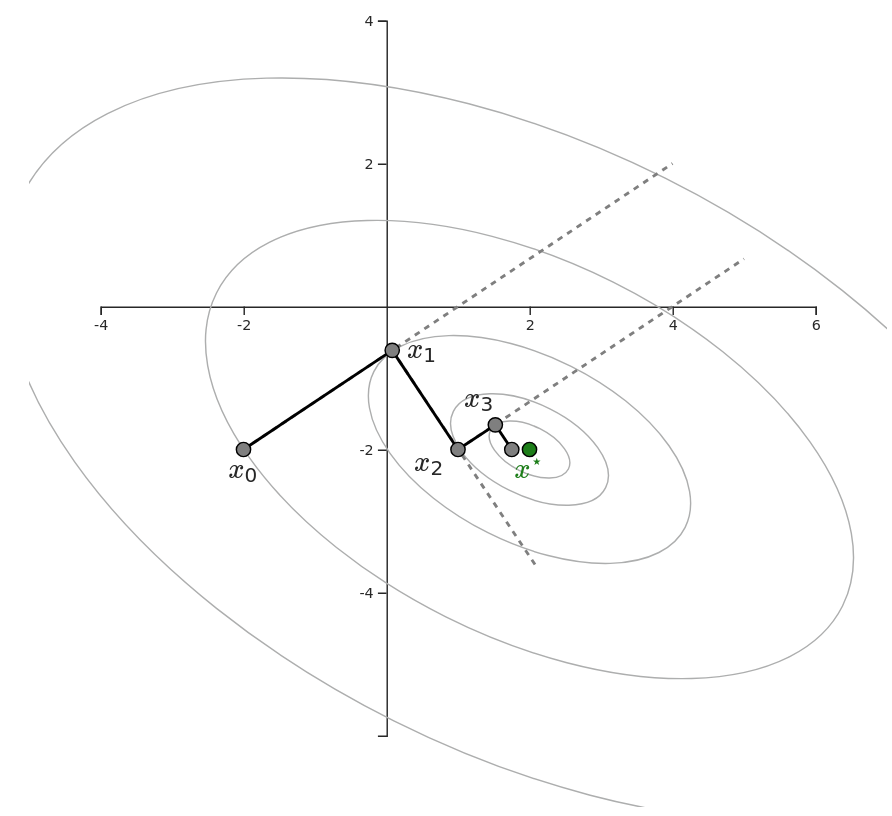
\includegraphics[width=0.7\textwidth]{./atelier/img/gradient_descent.png}
\caption{Approximation des Minimierers einer Funktion $F$ in zwei Variablen mit Hilfe des adaptiven Gradientenverfahrens \eqref{eq:gradient_descent_adaptive}.}
\label{fig:gradient_descent_adaptive}
\end{figure}
In Abbildung \ref{fig:gradient_descent_adaptive} ist ein typischer Verlauf des adaptiven Gradientenverfahrens in Algorithmus \ref{alg:gradient_descent_adaptive} bei der Minimierung einer Funktion $F \colon \mathbb{R}^2 \rightarrow \mathbb{R}$ zu sehen. 
Man erkennt, dass die Schrittweiten immer kleiner werden, je näher man sich dem lokalen Minimum $x_*$ nähert.
Außerdem sieht man, dass die Richtung des steilsten Gradientenabstiegs immer orthogonal zu den Niveaulinien der zu minimierenden Funktion steht.

\begin{remark}{}{}
Das in diesem Abschnitt beschriebene Gradientenabstiegsverfahren mit adaptiver Schrittweite $\tau_k > 0$ ist ein gängiger Algorithmus zur Minimierung einer Funktion $F$, wenn deren Ableitung $\nabla F$ bekannt und numerisch günstig zu berechnen ist. 
Dennoch gibt es Situationen in denen es ratsam ist alternative Optimierungsalgorithmen zu verwenden. 
Zum Beispiel ist ein häufiges Problem des Gradientenverfahrens die starke Verlangsamung in der Nähe eines Sattelpunktes, was zu sehr langen Laufzeiten des Algorithmus führt. 
Außerdem passiert die Minimierung einer Funktion $F$ mit Hilfe des Gradientenabstiegsverfahrens in der Regel entlang eines Zickzack-Pfades (siehe Abbildung \ref{fig:gradient_descent_adaptive}), welcher in den meisten Fällen offensichtlich suboptimal ist. 
Aus diesen Gründen wollen wir uns in den nächsten Abschnitten mit alternativen Minimierungsmethoden beschäftigen.
\end{remark}

\subsection{Koordinatenabstiegsverfahren}
\label{ss:coordinate_descent}
Eine weitere Variante des in Kapitel \ref{ss:gradient_descent} behandelten Gradientenabstiegsverfahrens ist das \textit{Koordinatenabstiegsverfahren} (im Englischen: \textit{coordinate descent} (CD)). 

Die grundlegende Idee des Koordinatenabstiegsverfahrens ist es in jedem Schritt des Iterationsschemas eine \textit{Koordinatenrichtung} auszuwählen und einen Abstieg in diese Richtung durchzuführen. 
Damit lässt sich ein möglicherweise kompliziertes multivariates Optimierungsproblem durch eine Reihe von einfachen univariaten Optimierungsproblemen behandeln.
Die Auswahl der Koordinatenrichtung kann entweder mit Hilfe einer Auswahlregel, z.B. mit einem Rundlaufverfahren, oder aber zufällig geschehen.

Wir wollen im Folgenden den Fall einer zufälligen Wahl der Koordinatenrichtung diskutieren.
Für einen zufälligen Index $j \in \lbrace 1,\ldots,n\rbrace$ und den entsprechenden zufälligen Einheitsvektor $\vec{e}_j \in \mathbb{R}^n$ lässt sich das Koordinatenabstiegsverfahren schreiben als:
\begin{equation}
\label{eq:coordinate_descent_stochastic}
x_{k+1} \ = \ x_k - \alpha_k \langle \nabla F(x_k), \vec{e_j} \rangle \vec{e_j} \ = \ x_k - \frac{\partial F}{\partial x^i}(x_k) \vec{e_j}.
\end{equation}
Das bedeutet, dass man in jeder Iteration nur eine Koordinate des aktuellen Parametervektors $x_k \in \Omega$ verändern muss.
Die Schrittweite $\alpha_k > 0$ in \eqref{eq:coordinate_descent_stochastic} kann hierbei ähnlich wie in Kapitel \ref{ss:gradient_descent} fest oder adaptiv gewählt werden.
Das Koordinatenabstiegsverfahren in \eqref{eq:coordinate_descent_stochastic} mit adaptiver Schrittweite lässt sich mit folgendem Algorithmus umsetzen.

~\\
\begin{algorithm}{Koordinatenabstiegsverfahren}{}
\label{alg:coordinate_descent_stochastic}
\begin{algorithmic}
\STATE \textbf{function} $[x^*, F(x^*)]= $\texttt{coordinateDescentStochastic}$(F,\nabla F, x_0, \alpha_0, \sigma, \epsilon$) \{
\STATE ~
\STATE \# Initialisierung
\STATE $\alpha_k = \alpha_0$
\STATE $x_k = x_0$
\STATE $F(x_{k+1}) = +$\texttt{Inf}
\STATE ~
\STATE \# Iteriere bis gewünschte Genauigkeit erreicht ist
\WHILE{$F(x_{k+1}) - F(x_k) > \epsilon$}
\STATE \# Wähle zufällige Koordinatenrichtung
\STATE $i = \texttt{randomDraw}([1:n])$
\STATE \# Berechne Richtungsableitung
\STATE $\vec{p}_k = \frac{\partial}{\partial x^i}F(x_k)$
\WHILE{$ F(x_k - \alpha_k \vec{p}_k / ||\vec{p}_k|| ) > F(x_k)$}
%\STATE ~
\STATE \# Verringere Schrittweite um Faktor $\sigma$
\STATE $\alpha_k = \sigma\alpha_k$
%\STATE ~
\ENDWHILE
\STATE \# Update in Richtung des größten Gradientenabstiegs
\STATE $x_{k+1} = x_k - \alpha_k \vec{p}_k / ||\vec{p}_k|| $
%\STATE ~
\ENDWHILE
\STATE ~
\STATE \# Ausgabe des letzten Punktes
\STATE $x^* = x_k$
\STATE $F(x^*) = F(x_k)$
\STATE \}
\end{algorithmic}
\end{algorithm}

%\textbf{ToDo: Abbildung erstellen}

Das Koordinatenabstiegsverfahren benötigt in der Regel deutlich mehr Iterationen als das normale Gradientenabstiegsverfahren und beschreibt häufig noch mehr einen Zickzack-Pfad bei der Minimierung.%, wie man in Abbildung \ref{fig:coordinate_descent_stochastic} sehen kann.
Dennoch bietet das Verfahren Vorteile gegenüber dem Gradientenabstiegsverfahren gerade in Optimierungsproblemen mit vielen Variablen, da jedes eindimensionale Optimierungsproblem wesentlich leichter zu lösen ist als die Berechnung des gesamten Gradienten in jedem Schritt. 

\begin{remark}{}{}
Um den Zufallseffekten und den damit verbundenen Zickzack Pfad bei der Minimierung der Funktion $F$ durch das Koordinatenabstiegsverfahren entgegen zu wirken, kann man einen Kompromiss zwischen der Verwendung einer einzelnen Koordinatenrichtung und dem gesamten Gradienten eingehen. 
Hierbei spricht man von den sogenannten \textit{Blockkoordinatenabtiegsverfahren} (im Englischen \textit{block coordinate descent} (BCD)).
Hierbei wählt man zuerst die Größe $s \in \lbrace 1,\ldots,n\rbrace$ der Koordinatenblöcke, d.h., die Größe der Teilmenge der verwendeten Richtungsableitungen des Gradienten $\nabla F$. Anschließend wird in jedem Schritt ein Block an Koordinatenrichtungen deterministisch oder zufällig ausgewählt und in dessen Richtung minimiert.
Für eine zufällige Wahl der Koordinatenblöcke ergibt sich somit:
\begin{equation}
\label{eq:block_coordinate_descent}
x_{k+1} \ = \ x_k - \alpha_k \langle \nabla F(x_k), \sum_{i=1}^s\vec{e}_{\sigma(i)} \rangle \sum_{i=1}^s\vec{e}_{\sigma(i)}.
\end{equation}
Hierbei ist $\sigma \colon \lbrace1,\ldots,n\rbrace \rightarrow \ \lbrace1,\ldots,n\rbrace$ eine zufällige Permutation der Indizes $1,\ldots,n$.
Es ist klar, dass das Koordinatenabstiegsverfahren in \eqref{eq:coordinate_descent_stochastic} und das normale Gradientenabstiegsverfahren in \eqref{eq:gradient_descent_adaptive} Spezialfälle des Blockkoordinatenabstiegsverfahrens in \eqref{eq:block_coordinate_descent} für Blockgrößen $s = 1$ und $s=n$ sind.
\end{remark}

\subsection{Stochastisches Gradientenabstiegsverfahren}
\label{ss:stochastic_gradient_descent}
Eine aktuell weit verbreitete Variante des Gradientenabstiegsverfahrens in \eqref{eq:gradient_descent_adaptive} ist das \textit{stochastische Gradientenabstiegsverfahren} (im Englischen: \textit{stochastic gradient descent} (SGD)). 
Wie der Name schon verrät handelt es sich hierbei nicht um einen deterministischen Algorithmus.
Das bedeutet, dass man bei mehrmaliger Anwendung des Verfahrens bei gleichbleibenden Startbedingungen in der Regel unterschiedliche Ergebnisse in unterschiedlichen Laufzeiten erhält.
Was auf den ersten Blick wie ein Nachteil wirkt, kann in manchen Fällen jedoch praktische Eigenschaften mit sich bringen.
So kann die Zufallsnatur des stochastischen Gradientenverfahrens dazu führen, dass Sattelpunkte und schlechte, lokale Minima der Funktion durch die Folge der Punkte vermieden werden.
Das Verfahren findet aktuell vor allem beim Training von neuronalen Netzen bei der sogenannten \textit{Backpropagation} in verschiedenen Variationen Anwendung, da man hierdurch dem bekannten Problem des \textit{Übertrainierens} des neuronalen Netzes entgegen wirken kann.

Beim stochastischen Gradientenverfahren geht man davon aus, dass sich die zu minimierende Zielfunktion $F \colon \Omega \rightarrow \mathbb{R}$ als eine Summe der folgenden Gestalt schreiben lässt:
\begin{equation}
\label{eq:objective_function_sum}
F(x) \ = \ \sum_{i=1}^m F_i(x), \quad \text{ für alle } x \in \Omega.
\end{equation} 
Solche Zielfunktionen treten natürlicherweise in vielen Problemstellungen auf, zum Beispiel bei Maximimum-Likelihood Ansätzen oder der Methode der kleinsten Quadrate.
Im Bereich des maschinellen Lernens lässt sich der Trainingsfehler über alle Trainingsdaten in der Regel als eine solche Summe  schreiben.
In diesem Fall lässt sich das normale Gradientenabstiegsverfahren in \eqref{eq:gradient_descent_adaptive} umschreiben zu:
\begin{equation}
\label{eq:gradient_descent_sum}
x_{k+1} \ = \ x_k - \alpha_k \frac{\nabla F(x_k)}{||\nabla F(x_k)||} \ = \ x_k - \alpha_k \frac{\sum_{i=1}^m\nabla F_i(x_k)}{||\sum_{i=1}^m\nabla F_i(x_k)||}, \quad \alpha_k > 0 .
\end{equation}

Die Idee des stochastischen Gradientenverfahrens ist es nun einen zufälligen Summanden aus \eqref{eq:objective_function_sum} zu wählen und nur den Gradienten bezüglich dieses Summanden zu betrachten.
Durch diese starke Vereinfachung von \eqref{eq:gradient_descent_sum} führt man mit einem zufällig ausgewählten Index $j \in \lbrace 1,\ldots,m\rbrace$ nun einen Gradientenabstieg der Form
\begin{equation}
\label{eq:stochastic_gradient_descent}
x_{k+1} \ = \ x_k - \alpha_k \frac{\nabla F_j(x_k)}{||\nabla F_j(x_k)||}, \quad \alpha_k > 0
\end{equation}
durch.
\begin{remark}{}{}
Ähnlich wie im Fall des Koordinatenabstiegsverfahrens in Kapitel \ref{ss:coordinate_descent}, gibt es auch beim stochastischen Gradientenverfahren die Möglichkeit einen Kompromiss zwischen dem normalen Gradientenabstieg in \eqref{eq:gradient_descent_control} und dem auf einen Summanden beschränkten Gradientenabstieg \eqref{eq:stochastic_gradient_descent} einzugehen. 
Indem man eine zufällige Untermenge von fester Größe $s \in \lbrace 1,\ldots,m\rbrace$ von Summanden von $F$ auswählt, lässt sich das sogenannte \textit{stochastische Minibatch-Gradientenabstiegsverfahren} formulieren:
\begin{equation*}
x_{k+1} = x_k - \alpha_k \frac{\sum_{i=1}^s\nabla F_{\sigma(i)}(x_k)}{||\sum_{i=1}^s\nabla F_{\sigma(i)}(x_k)||}, \quad \alpha_k > 0 .
\end{equation*}
Hierbei ist $\sigma \colon \lbrace 1,\ldots,m\rbrace \rightarrow \lbrace 1,\ldots,m\rbrace$ eine zufällige Permutation der Indizes $1,\ldots,m$.
\end{remark}

\subsection{Newton Verfahren}
\label{ss:newton}
In diesem Abschnitt wollen wir uns das bereits bekannte Newton-Verfahren in Erinnerung rufen und dieses geeignet zur Optimierung von nichtlinearen Funktionen verallgemeinern. 
In Kapitel $5.1$ der Vorlesung \glqq Einführung in die Numerik\grqq haben wir das Newton Verfahren zur Approximation von Nullstellen nichtlinearer Gleichungssysteme hergeleitet. 
Aus der Taylorentwicklung einer nichtlinearen Nullstellengleichung $F(x^*) = 0$ von der Form
\begin{equation*}
0 \ = \ F(x^*) \ = \ F(x) + (x^* - x) F'(x) + \mathcal{O}(F'').
\end{equation*}
haben wir die folgende Fixpunktfunktion als Approximation erster Ordnung angegeben: 
\begin{equation}
\label{eq:newton_fixpunkt}
G(x) \ = \ x - (F'(x))^{-1} F(x), \quad \text{ für } F'(x) \neq 0.
\end{equation}
Hierbei haben wir die Fixpunktgleichung als erfüllt gesehen, wenn wir ein $x^* \in \Omega$ gefunden haben, so dass die linke und rechte Seite von \eqref{eq:newton_fixpunkt} übereinstimmen. Unter dieser Beobachtung haben wir das \textit{Newton-Verfahren} als iteratives Schema zur Bestimmung eines solchen Fixpunktes $x^* \in \Omega$ hergeleitet:
\begin{equation}
x_{k+1} \ = \ x_k - \frac{F(x_k)}{F'(x_k)}.
\end{equation}
Hierfür benötigten wir einen geeigneten Startwert $x_0 \in \Omega$ in einer lokalen Umgebung $U \subset \Omega$ des Fixpunktes $x^* \in U$. Der folgende Satz Bedingungen für die lokale Konvergenz des Newton-Verfahrens. 
\begin{theorem}{}{}
Sei $F: \R^n \rightarrow \R^n$ in einer Umgebung von $\overline{x}$ stetig differenzierbar,  $F'$ lokal Lipschitz stetig , $F(\overline{x}) = 0$ und  $F'(\overline{x})$  regul\"ar. Dann existiert eine Umgebung $B_R(\overline{x})$, sodass das Newton-Verfahren f\"ur jeden Startwert $x_0 \in B_R(\overline{x})$ konvergiert, d.h. $x_k \rightarrow \overline{x}$.
\end{theorem}
\begin{proof}
Siehe \cite[Satz 5.7]{numerik1}.
\end{proof}

Anstatt nun eine Nullstelle der Funktion $F$ zu suchen, wollen wir das Newton-Verfahren nutzen, um eine Nullstelle des Gradienten $\nabla F$, d.h. einen stationären Punkt zu approximieren und damit die notwendigen Optimalitätsbedingungen zu erfüllen.
Im Folgenden sei $\Omega \subset \mathbb{R}^n$ ein offenes, zusammenhängendes Gebiet und $F \colon \Omega \rightarrow \mathbb{R}$ eine differenzierbare, reellwertige Funktion.
Wir betrachten wieder die Taylorapproximation der Funktion $F$ in eine Abstiegsrichtung $x_k + \vec{p} \in \Omega$ des allgemeinen Iterationsschemas \eqref{eq:abstiegsverfahren} aber berücksichtigen diesmal auch Terme von zweiter Ordnung:
\begin{equation}
\label{eq:modellfunktion}
F(x_k + \vec{p}) \ \approx \ F(x_k) + \langle \vec{p}, \nabla F(x_k) \rangle + \frac{1}{2} \langle \vec{p}, \nabla^2F(x_k)\vec{p} \rangle \ \eqqcolon \ m_k(\vec{p}).
\end{equation}
Wenn wir für den Moment davon ausgehen, dass die Hessematrix $\nabla^2 F(x_k)$ positiv definit ist, so können wir ein eindeutiges Minimum der Funktion $m_k(\vec{p})$ wie folgt bestimmen:
\begin{equation}
\label{eq:newton_richtung}
\vec{p} \ = \ -(\nabla^2 F(x_k))^{-1} \nabla F(x_k).
\end{equation}
Die Richtung $\vec{p} \in \mathbb{R}^n / \lbrace 0 \rbrace$ in \eqref{eq:newton_richtung} wird auch \emph{Newton-Richtung} genannt.
Mit ihr lässt sich ein iteratives Abstiegsverfahren für einen initialen Punkt $x_0 \in \Omega$, welcher geeignet in der Nähe des stationären Punktes $x^* \in \Omega$ gewählt wird, wie folgt konstruieren:
\begin{equation}
\label{eq:newton_abstieg}
x_{k+1} \ = \ x_k + \vec{p} \ = \ x_k - (\nabla^2 F(x_k))^{-1} \nabla F(x_k).
\end{equation}
Damit das Newton-Abstiegsverfahren in \eqref{eq:newton_abstieg} überhaupt sinnvoll ist, müssen wir fordern, dass die Hessematrix in jedem Punkt $x_k \in \Omega$ der Iterationsfolge invertierbar ist.
Um sicher zu gehen, dass es sich tatsächlich um eine Abstiegsrichtung handelt müssen wir fordern, dass die Hessematrix $\nabla^2 F(x_k)$ nicht nur invertierbar für alle $x_k \in \Omega$ der Iterationsfolge ist, sondern auch positiv definit in jedem Punkt $x_k$ ist. Denn dann ergibt eine Taylorapproximation zweiter Ordnung die folgende Abschätzung:
\begin{equation*}
\begin{split}
F(x_{k+1}) \ &= \ F(x_k + \vec{p}) \ \approx \ F(x_k) + \langle p, \nabla F(x_k) \rangle + \frac{1}{2} \langle \vec{p}, \nabla^2F(x_k) \vec{p} \rangle \\
\ &= \ F(x_k) - \langle (\nabla^2 F(x_k))^{-1} \nabla F(x_k), \nabla F(x_k) \rangle + \frac{1}{2} \langle \vec{p}, \nabla^2F(x_k) \vec{p} \rangle\\
\ &= \ F(x_k) - \langle (\nabla^2 F(x_k))^{-1} \nabla^2 F(x_k) \vec{p}, \nabla^2 F(x_k) \vec{p} \rangle + \frac{1}{2} \langle \vec{p}, \nabla^2F(x_k) \vec{p} \rangle \\
\ &= \ F(x_k) - \frac{1}{2} \underbrace{\langle \vec{p}, \nabla^2 F(x_k) \vec{p}}_{>~0} \rangle.
\end{split}
\end{equation*}
Wir sehen also, dass wir einen echten Abstieg der Funktionswerte erhalten, wenn die Hessematrix $\nabla^2 F(x_k)$ positiv definit ist für alle $x_k \in \Omega$ der Iterationsfolge. 
Sollte die Hessematrix nicht positiv definit in einem Punkt $x_k$ der Iterationsfolge sein, so muss zumindest eine Abnahme der Funktionswerte vorliegen, d.h., es muss für die Newton-Abstiegsrichtung gelten:
\begin{equation*}
\langle (\nabla^2F(x_k))^{-1} \nabla F(x_k), \nabla F(x_k) \rangle \ > \ 0.
\end{equation*}
Sollte dies nicht der Fall sein, so existieren Methoden um dennoch einen Abstieg zu erzwingen, siehe zum Beispiel \cite[Kapitel 6]{nocedal_1999}. Auf diese werden wir jedoch im weiteren Verlauf der Vorlesung nicht näher eingehen.
\begin{remark}{}{}
Das Newton-Abstiegsverfahren in \eqref{eq:newton_abstieg} ist ein Abstiegsverfahren der Art \eqref{eq:abstiegsverfahren} dessen Schrittweite $\alpha_k$ durch die lokale Krümmung und die Ableitung der Funktion $F$ bestimmt ist. In diesem Fall können wir $\alpha_k \equiv 1$ für alle $k \in \mathbb{N}$ setzen.
Das Newton-Abstiegsverfahren konvergiert in der Regel \emph{quadratisch} gegen einen stationären Punkt $x^* \in \Omega$ mit $\nabla F(x^*)=0$, d.h. man erreicht sehr schnell eine hohe Genauigkeit bei der Approximation von $x^*$.
\end{remark}

\subsection{Quasi-Newton Verfahren}
\label{ss:quasi-newton}
Im Kapitel \ref{ss:newton} haben wir das Newton Verfahren zur iterativen Approximation eines stationären Punktes $x^* \in \Omega$ einer Funktion $F$ mit $\nabla F(x^*) = 0$ hergeleitet. 
Hierbei haben wir im Gegensatz zu den vorherigen numerischen Verfahren auch Ableitungen höherer Ordnung hinzugezogen. 
Dies führt in der Regel zu einem verbesserten Konvergenzverhalten im Vergleich zu den Verfahren, die nur die lokale Ableitung $\nabla F$ der Funktion $F$ verwenden.
Dennoch ist das Newton Verfahren aus numerischer Sicht noch nicht ideal, da einige Probleme mit sich bringt.
Zuerst mussten wir fordern, dass die Hessematrix $\nabla^2 F(x_k)$ in jedem Punkt des Iterationsverfahrens positiv definit ist, da ansonsten kein Abstieg der Funktionswerte garantiert werden kann.
Zweitens muss für die Berechnung der Newton-Richtung in \eqref{eq:newton_richtung} zuerst die Hessematrix bestimmt und anschließend invertiert werden.
Dies ist aus Effizienzgründen ungewünscht, da die Inversion einer $n \times n$-Matrix in $\mathcal{O}(n^3)$ Rechenoperationen liegt.
Da die Bestimmung und die Inversion der Hessematrix in jedem Iterationsschritt passieren müssen, ist das Newton Verfahren nicht empfehlenswert für die numerische Optimierung.

Eine naheliegende Idee ist es nun die echte Hessematrix in jedem Iterationsschritt durch eine geeignete Matrix zu approximieren, so dass der numerische Aufwand geringer wird, d.h., wir suchen nach einer Matrix
\begin{equation}
\label{eq:matrix_bk}
B_k \approx \nabla^2 F(x_k).
\end{equation}
Damit können wir die Modellfunktion $m_k(\vec{p})$ in \eqref{eq:modellfunktion} schreiben als:
\begin{equation*}
m_k(\vec{p}) \ = \ F(x_k) + \langle \nabla F(x_k), \vec{p} + \frac{1}{2} \langle \vec{p}, B_k \vec{p} \rangle,
\end{equation*}
das heißt, wir approximieren die Zielfunktion $F$ im $k$-ten Iterationsschritt entlang der Richtung $\vec{p} \in \mathbb{R}^n$ lokal durch eine quadratische Funktion.
Für sehr kleine Schrittweiten können wir davon ausgehen, dass der Fehler dieser Approximation gering ist, da wir davon ausgehen, dass $F$ stetig differenzierbar in einer lokalen Umgebung $U \subset \Omega$ des stationären Punktes $x^* \in \Omega$ ist und für $\vec{p} = 0$ die Approximation exakt ist, da
\begin{equation*}
m_k(0) \ = \ F(x_k).
\end{equation*}
Wenn wir fordern, dass $B_k$ in \eqref{eq:matrix_bk} eine positiv definite Matrix ist, so lässt sich ein Abstiegsschritt des Iterationsverfahrens \eqref{eq:abstiegsverfahren} analog zur Herleitung des Newton Abstiegsverfahrens in Kapitel \ref{ss:newton} angeben als:
\begin{equation}
\label{eq:quasi-newton-abstieg}
x_{k+1} \ = \ x_k + \alpha_k \vec{p}_k, \qquad \vec{p}_k \ = \ -B_k^{-1} \nabla F(x_k).
\end{equation}
Die sogenannten \emph{Quasi-Newton Verfahren} verfolgen diesen Ansatz. 
Durch die Approximation der echten Hessematrix verlieren Quasi-Newton Verfahren an Genauigkeit, wodurch ihre Konvergenzgeschwindigkeit superlinear anstatt quadratisch ist. 
Dafür gewinnen sie zusätzliche Geschwindigkeit durch die Vermeidung der Bestimmung und Inversion von $\nabla^2 F(x_k)$.
Der Vorteil der Quasi-Newton Methoden ist es, dass man nur den Gradienten $\nabla F$ für einen Schritt des numerischen Optimierungsverfahrens benötigt und keine expliziten Informationen über die zweiten Ableitungen.
Dadurch werden sie in bestimmten Problemen sogar effizienter bei der Approximation eines stationären Punktes als das Newton Abstiegsverfahren in Kapitel \ref{ss:newton}.

Die entscheidende Frage bei der Konstruktion eines Quasi-Newton Abstiegsverfahrens der Form \eqref{eq:quasi-newton-abstieg} ist es, wie die positiv definite Matrix $B_k$ in jedem Schritt möglichst effizient bestimmt werden kann. 
Anstatt die Näherung $B_k$ der Hessematrix $\nabla^2 F(x_k$ in jedem Schritt von Grund auf neu zu berechnen, wäre es wünschenswert ein initiales $B_0$ in jedem Schritt des Iterationsverfahrens zu aktualisieren.
Hierbei ist es möglich die durch den Iterationsschritt erhaltenen Informationen über den Gradienten $\nabla F$ zu Hilfe zu nehmen.
Wir nehmen an, wir haben bereits einen Abstiegsschritt durchgeführt und so einen neuen Punkt $x_{k+1} = x_k + \alpha_k\vec{p}$ erhalten.
Unsere quadratische Approximation in diesem neuen Punkt für eine neue Richtung $\vec{p} \in \mathbb{R}^n$ sieht dementsprechend wie folgt aus:
\begin{equation*}
m_{k+1}(\vec{p}) \ = \ F(x_{k+1}) + \langle \nabla F(x_{k+1}), \vec{p} \rangle + \frac{1}{2}\langle \vec{p}, B_{k+1}\vec{p} \rangle.
\end{equation*}
Eine Forderung, die man nun die Modellfunktion $m_{k+1}$ stellen kann ist, dass ihre Ableitung mit der Ableitung der Zielfunktion $F$ in den letzten beiden Punkten $x_k$ und $x_{k+1}$ übereinstimmt.
Da
\begin{equation*}
\nabla m_{k+1}(0) \ = \ \nabla F(x_{k+1})
\end{equation*}
gilt, ist eine der beiden Forderungen automatisch erfüllt.
Für die zweite Forderung können wir nutzen, dass $x_k = x_{k+1} - \alpha_k \vec{p}_k$ gilt und wir somit erhalten:
\begin{equation}
\label{eq:quasi-newton_forderung}
\nabla m_{k+1}(-\alpha_k\vec{p}_k) \ = \ \nabla F(x_{k+1}) - \alpha_k B_{k+1}\vec{p}_k \ \overset{!}{=} \ \nabla F(x_k).
\end{equation}
Durch Umstellen von \eqref{eq:quasi-newton_forderung} erhalten wir die Bedingung
\begin{equation*}
B_{k+1}\alpha_k \vec{p}_k \ = \ B_{k+1}(x_{k+1} - x_k) \ \overset{!}{=} \ \nabla F(x_{k+1}) - \nabla F(x_k).
\end{equation*}
Eine vernünftige Wahl der Matrix $B_{k+1}$ in \eqref{eq:matrix_bk} sollte diese Eigenschaft, auch bekannt als \textbf{Sekantengleichung}, versuchen zu imitieren.
Im eindimensionalen Fall mit $F \colon \Omega \subset \mathbb{R} \rightarrow \mathbb{R}$ bedeutet die Sekantengleichung nichts anderes, als dass der Faktor $B_{k+1}$ eine Approximation des zweiten Ableitung von $F$ im Sinne eines Differenzenquotienten ist, d.h., im Fall $n=1$ soll gelten:
\begin{equation*}
B_{k+1} \ \overset{!}{=} \ \frac{F'(x_{k+1})-F'(x_k)}{x_{k+1} - x_k}.
\end{equation*}

Für unser allgemeines Quasi-Newton Verfahren in \eqref{eq:quasi-newton-abstieg} suchen wir also einen Weg die bereits bekannte Approximation der Hessematrix $B_k \approx \nabla^2F(x_k)$ zu einer Matrix $B_{k+1}$ aktualisieren, so dass der folgende Zusammenhang für den nächsten Punkt $x_{k+1} \in \Omega$ erfüllt wird:
\begin{equation}
\label{eq:sekantengleichung}
B_{k+1} s_k \ = \ y_k,
\end{equation}
wobei
\begin{equation*}
s_k \ = \ x_{k+1} - x_k, \qquad y_k = \nabla F(x_{k+1}) - \nabla F(x_k).
\end{equation*}
Es wird klar, dass diese Forderung alleine nicht genügt für die Konstruktion eines Abstiegsverfahrens.
Um die positive Definitheit der Matrix $B_{k+1}$ in Schrittrichtung $\alpha\vec{p}_k$ zu gewährleisten müssen wir fordern, dass die Vektoren $y_k$ und $s_k$ die sogenannte \textbf{Krümmungsbedingung} erfüllen:
\begin{equation}
\label{eq:kruemmungsbedingung}
\langle s_k, y_k \rangle \ > \ 0.
\end{equation}
Dies ist eine hinreichende Bedingung für die positive Definitheit von $B_{k+1}$ bezüglich der Richtung $\alpha_k \vec{p}_k$, da wir einfach die Sekantengleichung \eqref{eq:sekantengleichung} von links mit dem Vektor $s_k^T$ multiplizieren können und so erhalten wir mit der Forderung \eqref{eq:kruemmungsbedingung} schon:
\begin{equation*}
\langle s_k, B_{k+1}s_k \rangle \ = \ \langle s_k, y_k \rangle \ > \ 0.
\end{equation*}
\begin{remark}{}{}
Falls die Funktion $F$ strikt konvex ist, so ist die Krümmungsbedingung \eqref{eq:kruemmungsbedingung} für alle Punktepaare $x_k, x_{k+1} \in \Omega$ erfüllt und die Matrix $B_{k+1}$ wird damit positiv definit. Für nichtkonvexe Funktionen hingegen muss man die Krümmungsbedingung explizit forcieren, um ein Abstiegsverfahren zu erhalten.
\end{remark}

Falls die Krümmungsbedingung \eqref{eq:kruemmungsbedingung} erfüllt ist, so existiert mindestens eine Lösung $B_{k+1}$ der Sekantengleichung \eqref{eq:sekantengleichung}.
Man sieht ein, dass es in der Tat sogar unendlich viele Lösungen $B_{k+1}$ gibt, da eine symmetrische $n \times n$ Matrix $n(n+1)/2$ Freiheitsgrade besitzt und die Sekantengleichung \eqref{eq:sekantengleichung} nur $n$ Bedingungen an $B_{k+1}$ stellt.
Zusätzlich erhält man $n$ Bedingungen an $B_{k+1}$ durch die Forderung von positiver Definitheit, da alle $n$ Hauptminoren von $B_{k+1}$ positiv sein müssen.
Dies reicht jedoch nicht für die eindeutige Bestimmung der Matrix $B_{k+1}$.
Hierfür müssen wir zusätzlich fordern, dass die Matrix $B_{k+1}$ diejenige Matrix unter allen möglichen Lösungen ist, die der vorherigen Matrix $B_k$ am nächsten bezüglich eines geeigneten Maßes ist.
Das heißt wir suchen eine Lösung des folgenden Optimierungsproblems:
\begin{equation}
\label{eq:quasi-newton_optimization-problem}
\begin{split}
\min_{B} || B - B_k ||, \quad \text{ unter den Nebenbedingungen: } \\
B \ = \ B^T, \qquad B s_k \ = \ y_k, \qquad \langle \vec{p}, B\vec{p} \rangle > 0, \forall \vec{p} \in \mathbb{R}^n / \lbrace 0 \rbrace,
\end{split}
\end{equation}
wobei $s_k$ und $y_k$ definiert sind wie in der Sekantengleichung \eqref{eq:sekantengleichung}.
Man beachte, dass man eine unterschiedliche Lösung $B_{k+1}$ des Optimierungsproblems \eqref{eq:quasi-newton_optimization-problem} in Abhängigkeit der gewählten Matrixnorm erhält und somit auch ein unterschiedliches Quasi-Newton Verfahren herleiten kann.

\subsubsection{Das Davidon-Fletcher-Powell Verfahren}
Im ursprünglich im Jahr $1959$ von Davidon vorgeschlagenen Verfahren \cite{davidon_1959}, das im Übrigen bei der Erstbegutachtung abgelehnt wurde, wählt man für die Norm im Optimierungsproblem \eqref{eq:quasi-newton_optimization-problem} eine gewichtete Frobeniusnorm der Form
\begin{equation*}
||A||_W \ \coloneqq \ || W^\frac{1}{2}A W^\frac{1}{2} ||_F.
\end{equation*}
Die Gewichtungsmatrix $W$ dient dazu, dass das implizierte Quasi-Newton Verfahren zur Approximation eines stationären Punktes $x^* \in \Omega$ skalierungs-invariant wird. 
Hierzu wählt man eine beliebige Matrix für die die Relation $W y_k = s_k$ gilt, d.h., eine Matrix $W$, die sich wie die Inverse der Matrix $B$ in \eqref{eq:quasi-newton_optimization-problem} verhält.
Ein konkretes Beispiel solch eine Gewichtungsmatrix wäre $W \coloneqq G_k^{-1}$, wobei $G_k$ die durchschnittliche Hessematrix von $F$ entlang des letzten Abstiegsschritts von $x_k \rightarrow x_{k+1}$ ist mit
\begin{equation*}
G_k \ \coloneqq \ \int_0^1 \nabla^2 F(x_k + t \alpha_k \vec{p}_k)~\mathrm{d}t.
\end{equation*}
Mit der konkreten Wahl dieser Gewichtungsmatrix $W = G_k^{-1}$ wird die gewichtete Frobeniusnorm  dimensionslos und man erhält eine eindeutige Lösung des Optimierungsproblems \eqref{eq:quasi-newton_optimization-problem} wie folgt:
\begin{equation}
\label{eq:DFP}
B_{k+1} \ = \ (I-\gamma_k y_ks_k^T) B_k (I - \gamma_k s_k y_k^T) + \gamma_k y_k y_k^T, \quad \text{ mit } \gamma_k \ \coloneqq \ \frac{1}{\langle y_k, s_k \rangle}.
\end{equation}
Die Gleichung \eqref{eq:DFP} wird auch \textbf{DFP-Schritt} genannt, da sie zuerst von Davidon vorgeschlagen und später von Fletcher und Powell untersucht und verbreitet wurde.

Obwohl wir die explizite Berechnung der Hessematrix $\nabla^2 F(x_k)$ vermieden haben und die Aktualisierung der Matrix $B_k$ zu $B_{k+1}$ lediglich auf den Gradienteninformationen von $F$ basiert ist der numerische Aufwand bei direkter Verwendung von $B_{k+1}$ in \eqref{eq:DFP} noch zu hoch.
Das liegt daran, dass wir für einen Schritt des Quasi-Newton Verfahrens in \eqref{eq:quasi-newton-abstieg} die Inverse der Matrix $B_k$ benötigen und die Inversion einen numerischen Aufwand von $\mathcal{O}(n^3)$ besitzt.
Glücklicherweise gibt es einen Trick, wie wir die Inverse von $B_k$ in jedem Schritt des Iterationsverfahrens numerisch günstig erhalten können.
Sei $H_k \coloneqq B_k^{-1}$, dann können wir die sogenannte Sherman-Morrison-Woodbury Formel auf Gleichung \eqref{eq:DFP} anwenden um die neue Inverse $H_{k+1}$ durch eine Aktualisierung der Matrix $H_k$ zu berechnen:
\begin{equation}
\label{eq:smw-formel}
H_{k+1} \ = \ H_k - \frac{H_k y_k y_k^T H_k}{\langle y_k, H_k y_k\rangle} + \frac{s_k s_k^T}{\langle y_k, s_k \rangle} . 
\end{equation}
Wie man einssieht liegt der numerische Rechenaufwand für das Update von $H_{k+1}$ in \eqref{eq:smw-formel} in $\mathcal{O}(n^2)$.
Es fällt außerdem auf, dass $H_k$ nur durch die Addition zweier Matrizen mit Rang $1$ verändert wird, also insgesamt eine Änderung von höchstes Rang $2$ erfährt.
Das passt gut zu der Forderung, dass wir erwarten, dass sich die Approximation der Hessematrix $\nabla^2 F$ in einer lokalen Umgebung nur wenig ändert.

\subsubsection{Das Broyden--Fletcher--Goldfarb--Shanno Verfahren}
Das Davidon--Fletcher--Powell Verfahren wurde trotz seiner Effektivität bald schon durch ein Verfahren abgeläst, dass noch besser war und bis heute zu den effizientesten Quasi-Newton Verfahren gehört: das Broyden--Fletcher--Goldfard--Shanno (BFGS) Verfahren.
Die Idee des BFGS Verfahrens leitet sich unmittelbar aus der Idee des DFP Verfahren ab.
Anstatt das Optimierungsproblem \eqref{eq:quasi-newton_optimization-problem} mit bestimmten Bedingungen an die Approximation $B_{k+1}$ der Hessematrix $\nabla^2 F(x_k)$ zu stellen, versucht man direkt die Inverse der Hessematrix $(\nabla^2 F(x_k))^{-1}$ geeignet zu approximieren.
Hierfür nehmen wir an, dass wir eine Matrix $H_{k+1}$ als geringfügige Aktualisierung einer bereits vorher bestimmten Matrix $H_k$ suchen, die gleichzeitig symmetrisch und positiv definit ist und zusätzlich die Sekantenbedingung in umgeschriebener Form erfüllt:
\begin{equation*}
H_{k+1}y_k \ = \ s_k.
\end{equation*}
Hierzu formuliert man ein analoges Optimierungsproblem zu \eqref{eq:quasi-newton_optimization-problem} von der Form:
\begin{equation}
\label{eq:bfgs_optimierungsproblem}
\begin{split}
\min_{H} || H - H_k ||, \quad \text{ unter den Nebenbedingungen: } \\
H \ = \ H^T, \qquad H y_k \ = \ s_k, \qquad \langle \vec{p}, H\vec{p} \rangle > 0, \forall \vec{p} \in \mathbb{R}^n / \lbrace 0 \rbrace.
\end{split}
\end{equation}
Unter der Verwendung der gewichteten Frobeniusnorm und einer beliebigen Gewichtsfunktion, die die Sekantengleichung $Ws_k = y_k$ erfüllt, erhält man wiederum die eindeutige Lösung des Minimierungsproblems \eqref{eq:bfgs_optimierungsproblem} als:
\begin{equation}
\label{eq:bfgs}
H_{k+1} \ = \ (I - \rho_k s_k y_k^T) H_k (I - \rho_k y_k s_k^T) + \rho_k s_k s_k^T, \quad \text{ mit } \rho_k \coloneqq \frac{1}{\langle y_k, s_k \rangle}.
\end{equation}
Das Update der Matrix $H_k$ in \eqref{eq:bfgs} kann numerisch in $\mathcal{O}(n^2)$ durchgeführt werden, was man schnell einsieht, wenn man das Produkt ausschreibt:
\begin{equation*}
H_{k+1} \ = \ H_k - H_k\rho_k y_k s_k^T - \rho_k s_k y_k^T H_k + \rho_k s_k y_k^T H_k \rho_k y_k s_k^T + \rho_k s_k s_k^T.
\end{equation*}
In dieser Schreibweise sieht man gut, dass man lediglich Skalarprodukte in $\mathcal{O(n)}$, Matrix-Vektor Multiplikationen in $\mathcal{O}(n^2)$ und dyadische Produkte in $\mathcal{O(n^2)}$ berechnen muss.
Im Gegensatz hierzu würde eine naive Implementierung des BFGS-Updates in \eqref{eq:bfgs} zu einem numerischen Aufwand von $\mathcal{O}(n^3)$ führen.

Abschließend bleibt die Frage was eine gute Initialisierung der Matrix $H_0$ ist.
Idealerweise hat man bereits Informationen über die Inverse der Hessematrix $(\nabla^2 F(x_0))^{-1}$ im Initialisierungspunkt $x_0 \in \Omega$, zum Beispiel durch eine numerische Approximation mittels finiter Differenzen (später in der Vorlesung!).
Andererseits erwarten wir, dass die Aktualisierung von $H_k$ im $k$-ten Schritt des Iterationsverfahrens \eqref{eq:bfgs} zu $H_{k+1}$ die aktuellen Informationen über den Verlauf der Gradienten $\nabla F(x_k)$ und $\nabla F(x_{k+1})$ berücksichtigt.
Darum ist eine häufige Wahl von $H_0$ die Initialisierung als Einheitsmatrix $I_n$ oder ein Vielfaches der Einheitsmatrix, wobei die Vorfaktoren der Diagonaleinträge entsprechend der Skalierung der Variablen gewählt werden.

\section{Verfahren der konjugierten Gradienten}
\label{s:cg_verfahren}
Im Folgenden wollen wir uns mit einem besonders eleganten Verfahren der Optimierung beschäftigen: dem Verfahren der konjugierten Gradienten.
Ursprünglich wurde das Verfahren von Hestenes und Stiefel in \cite{hestenes_1952} im Jahr $1952$ vorgeschlagen.
Obwohl das Verfahren im Allgemeinen für die nichtlineare Optimierung eingesetzt werden kann, wird es insbesondere zur Lösung von großen linearen Gleichungssystemen $Ax = b$ mit symmetrischer, dünn besetzter, positiv definiter $n\times n$ Matrix $A$ eingesetzt.
Solche Gleichungssysteme treten zum Beispiel bei der numerischen Modellierung und Lösung partieller Differentialgleichungen auf.
Das Verfahren lässt sich in diesem Fall besonders anschaulich motivieren und herleiten.
Darum wollen wir uns im Folgenden auf das Lösen von großen linearen Gleichungssystemen $Ax=b$ konzentrieren.
Wir folgen bei der Herleitung des Verfahren der konjugierten Gradienten der didaktisch sehr gelungenen Arbeit von Jonathan Shewchuk in \cite{shewchuk_1994}.
Für eine ansprechende, interaktive Visualisierung des Verfahren der konjugierten Gradienten empfehlen wir den Mathematik Blog von Philipp Wacker \cite{wacker}.

\subsection{Problemstellung}
\label{ss:cg_problemstellung}
Sei im folgenden also $A \in \mathbb{R}^{n \times n}$ eine sehr große $n \times n$-Matrix und $b \in \mathbb{R}^n$ ein reeller Vektor.
Wir suchen einen unbekannten Vektor $x \in \mathbb{R}^n$, der das lineare Gleichungssystem
\begin{equation}
\label{eq:LGS}
Ax \ = \ b
\end{equation}
löst.
Wir suchen also nach denjenigen Koeffizienten, mit denen sich der Vektor $b$ als Linearkombination aus Spaltenvektoren der Matrix $A$ darstellen lässt. 
Diese Koeffizienten entsprechen den Einträgen des unbekannten Vektors $x$.
Aus der Vorlesung \glqq Einführung in die Numerik\grqq~ in \cite[Kapitel 2]{numerik1} ist bekannt, dass es genau dann eine eindeutige Lösung $x \in \mathbb{R}^n$ für die Gleichung \eqref{eq:LGS} gibt, falls die Determinante $\operatorname{det}(A) \neq 0$ ist.
Eine hinreichende Bedingung für die Eindeutigkeit des Lösungsvektors $x \in \mathbb{R}^n$ ist es also zu fordern, dass die Matrix $A$ symmetrisch und positiv definit ist.
Wir gehen also im Folgenden immer davon aus, dass $A$ eine symmetrische und positiv definite $n \times n$-Matrix ist.
In diesem Fall ist das Bestimmen einer Lösung von \eqref{eq:LGS} ein gut-gestelltes Problem und die Lösung ließe sich direkt angeben als:
\begin{equation*}
x \ = \ A^{-1}b.
\end{equation*}
Wie wir jedoch ebenfalls aus \cite[Kapitel 2]{numerik1} wissen ist die Inversion einer $n\times n$-Matrix $A \in \mathbb{R}^{n\times n}$ numerisch sehr aufwending und selbst unter Ausnutzung der Symmetrie lässt sich höchstens ein Verfahren mit Rechenaufwand $\mathcal{O}(\frac{1}{6}n^3)$ angeben.
Sollte die Dimension des Problems jedoch sehr groß sein (d.h. wir nehmen $n >> 1$ an), so ist eine direkte Lösung von \eqref{eq:LGS} mittels Inversion nicht durchführbar.
Glücklicherweise liefert uns das Verfahren der konjugierten Gradienten (neben anderen iterativen Lösungsalgorithmen) eine Möglichkeit das lineare Gleichungssystem numerisch zu lösen.

Hierzu betrachten wir zunächst ein quadratisches Optimierungsproblem der Form
\begin{equation}
\label{eq:quadratic_problem}
\min_{x\in \mathbb{R}^n} \frac{1}{2} \langle x, Ax \rangle - \langle b, x \rangle + c,
\end{equation}
wobei $A$ und $b$ wie im Fall des linearen Gleichungssystems in \eqref{eq:LGS} gewählt sind und $c \in \mathbb{R}$ eine beliebige, reelle Konstante ist.
Der folgende Satz liefert uns eine hilfreiche Aussage zur Lösung des ursprünglichen Problems.
\begin{theorem}{}{LGS_equivalent}
Das quadratische Minimierungsproblem in \eqref{eq:quadratic_problem} ist äquivalent zum ursprünglichen linearen Gleichungssystem in \eqref{eq:LGS}, d.h., jede Lösung von \eqref{eq:quadratic_problem} ist schon Lösung von \eqref{eq:LGS} und anders herum.
\end{theorem}
%
%
\begin{proof}
Für die erste Richtung des Beweises nehmen wir an, dass $x_* \in \mathbb{R}^n$ eine Lösung des linearen Gleichungssystems $Ax = b$ sei. 
Wir betrachten die hinreichenden Optimalitätsbedingungen zweiter Ordnung aus Satz \ref{thm:minimum_hinreichend} für das Minimierungsproblem \eqref{eq:quadratic_problem}. 
Hierzu suchen wir zunächst die stationären Punkte der Funktion $F \colon \mathbb{R}^n \rightarrow \mathbb{R}$ mit
\begin{equation*}
F(x) \ \coloneqq \ \frac{1}{2} \langle x, Ax \rangle - \langle b, x \rangle + c.
\end{equation*}
Der Gradient von $F$ lässt sich bestimmen als
\begin{equation*}
\nabla F(x) \ = \ \frac{1}{2}(A - A^T)x - b \ = \ Ax - b.
\end{equation*}
Alle stationären Punkte $x \in \mathbb{R}^n$ von $F$ mit $\nabla F(x) = 0$ sind also gerade die Lösungen des linearen Gleichungssystems $Ax = b$.
Damit ist $x_*$ nach Vorraussetzung also einziger stationärer Punkt von $F$.
Um zu zeigen, dass $x_* \in \mathbb{R}^n$ auch schon ein lokales Minimum von $F$ ist müssen wir noch die Hessematrix von $F$ betrachten, welche gegeben ist durch:
\begin{equation*}
\nabla^2 F(x) \ = \ A.
\end{equation*}
Da $A$ nach Vorraussetzung positiv definit ist, ist auch die Hessematrix $\nabla^2 F(x) = A$ positiv definit und somit sind die hinreichenden Kriterien für das vorliegen eines lokalen Minimums von $F$ im Punkt $x_* \in \mathbb{R}^n$ erfüllt.

Für die Rückrichtung des Beweises nehmen wir, dass $x_* \in \mathbb{R}^n$ ein lokales Minimum der Funktion $F$ ist.
Daraus können wir folgern, dass $x_*$ ein stationärer Punkt von $F$ ist und somit gelten muss:
\begin{equation*}
\nabla F(x_*) \ = \ A x_* - b \ = \ 0.
\end{equation*}
Das bedeutet aber schon, dass $x_* \in \mathbb{R}^n$ Lösung des linearen Gleichungssystems $Ax = b$ ist.
\end{proof}
Der Satz \ref{thm:LGS_equivalent} erlaubt es uns also ein quadratisches Optimierungsproblem der Form \eqref{eq:quadratic_problem} numerisch zu lösen anstatt einen unbekannten Lösungsvektor für ursprüngliche lineare Gleichungssystem \eqref{eq:LGS} zu finden.

Wir interessieren uns nun also für ein iteratives Verfahren, welches eine Folge von Punkten $x_0,x_1,\ldots \in \mathbb{R}^n$ konstruiert, die gegen ein Minimum von \eqref{eq:quadratic_problem} und somit gegen die eindeutige Lösung des linearen Gleichungssystems \eqref{eq:LGS} konvergiert.
Hierfür benötigen wir noch zusätzliche Notation, um das angestrebte Verfahren vernünftig zu beschreiben.
\begin{definition}{Fehler und Residuum}{residuum}
Sei $x_{k+1} = G(x_k)$ ein Iterationsverfahren, dass gegen ein lokales Minimum $x_* \in \mathbb{R}^n$ der quadratischen Funktion $F$ in \eqref{eq:quadratic_problem} konvergiert, d.h., $x_k \rightarrow x_*$ für $k \rightarrow \infty$. Dann können wir die beiden folgenden Begriffe definieren:
\begin{enumerate}[label=(\roman*)]
\item Wir bezeichnen den Vektor $e_k \in \mathbb{R}^n$ mit
\begin{equation*}
e_k \ \coloneqq \ x_k - x_*
\end{equation*}
als den aktuellen \emph{Fehler}, den man durch den aktuellen Punkt $x_k \in \mathbb{R}^n$ macht.
\item Wir bezeichnen den Vektor $r_k \in \mathbb{R}^n$ mit
\begin{equation*}
r_k \ \coloneqq \ b - Ax_k
\end{equation*}
als das aktuelle \emph{Residuum}, das man durch den aktuellen Punkt $x_k \in \mathbb{R}^n$ erhält. 
\end{enumerate}
\end{definition}
\begin{remark}{}{}
In Bezug auf Definition \ref{def:residuum} lassen sich folgende Aussagen festhalten:
\begin{enumerate}[label=(\roman*)]
\item Der Fehler $e_k \in \mathbb{R}^n$ ist eher abstrakter Natur und dient zur besseren Analyse des Verfahrens der konjugierten Gradienten. Explizit werden wir diesen Vektor jedoch nie bestimmen können innerhalb des Iterationsverfahrens, da wir dann schon fertig wären mit einem einfach Update der Form $x_* = x_k - e_k$.
\item Wie bereits im Beweis von Satz \ref{thm:LGS_equivalent} gesehen, lässt sich das Residuum $r_k \in \mathbb{R}^n$ außerdem wie folgt umschreiben:
\begin{equation*}
r_k \ = \ \underbrace{b - Ax_k}_{= -\nabla F(x_k)} \ = \ Ax_* - Ax_k \ = \ A (x_* - x_k) \ = \ -Ae_k.
\end{equation*}
Daher lässt sich das Residuum $r_k$ auch als die Richtung des stärksten Abstiegs interpretieren und es ist klar, dass $r_k$ immer orthogonal zu den Niveaulinien der Funktion $F$ steht.
\end{enumerate}
\end{remark}
Abbildung \ref{fig:residuum} illustriert anschaulich die geometrische Bedeutung der beiden in Definition \ref{def:residuum} eingeführten Vektoren.
Wie man unschwer erkennt zeigen Fehler und Residuum im Allgemeinen nicht in die selbe Richtung.
Das erklärt auch warum das Gradientenabstiegsverfahren in Kapitel \ref{ss:gradient_descent} selbst bei optimaler Schrittweite $alpha_k > 0$ nicht in einem Schritt die gesuchte Lösung $x_* \in \mathbb{R}^n$ erreicht.
\begin{figure}
\centering
\includegraphics[width=0.8\textwidth]{./atelier/img/residuum.png}
\caption{Visualisierung des Fehlers $e_0 \in \mathbb{R}^n$ und des Residuums $r_0 \in \mathbb{R}^n$ für einen Startpunkt $x_0 \in \mathbb{R}^n$.}
\label{fig:residuum}
\end{figure}

\subsection{Motivation}
\label{ss:motivation}
Um das Vorgehen beim Verfahren der konjugierten Gradienten zu motivieren rufen wir uns noch einmal das Gradientenabstiegsverfahren aus Kapitel \ref{ss:gradient_descent} in Erinnerung.
Nehmen wir an wir befinden uns im $k$-Schritt des Gradientenabstiegsverfahrens in Algorithmus \ref{alg:gradient_descent_adaptive} in einem Punkt $x_k \in \mathbb{R}^n$ und es sei eine Schrittweite $\alpha_k > 0$ gegeben.
Dann erhalten wir den nächsten Punkt $x_{k+1} \in \mathbb{R}^n$ der Iterationsfolge durch folgendes Update:
\begin{equation*}
x_{k+1} \ = \ x_k - \alpha_k \nabla F(x_k) \ = \ x_k + \alpha_k r_k,
\end{equation*}
wobei $r_k \in \mathbb{R}^n$ das aktuelle Residuum des Punktes $x_k$ bezeichnet.
Wir springen also in Richtung des steilsten Gradientenabstiegs einen Schritt der Länge $\alpha_k > 0$.
Da die Abstiegsrichtung in jedem Schritt $x_k \rightarrow x_{k+1}$ orthogonal zu den Niveaulinien von $F$ steht, erhält man typischerweise einen Zickzack-Pfad durch das Gradientenabstiegsverfahren (vgl. Abbildung \ref{fig:gradient_descent_adaptive}).
Um dieses typische Verhalten besser zu verstehen können wir eine Vorüberlegung zur Schrittweitenwahl für das quadratische Optimierungsproblem in \eqref{eq:quadratic_problem} machen.
Hierzu gehen wir analog zur Bestimmung der optimalen Schrittrichtung in Kapitel \ref{ss:gradient_descent} vor, nur dass wir diesmal die Schrittrichtung $\vec{p}_k \coloneqq -\nabla F(x_k)$ festhalten und bezüglich der unbekannten Schrittweite optimieren.
Wir gehen davon aus, dass wir das lokale Minimum von $F$ noch nicht erreicht haben, denn dann wäre $\alpha_k = 0$.
Wir suchen also eine Schrittweite $\alpha > 0$, so dass der Funktionswert $F(x_{k+1})$ entlang der Linie $x_k - \alpha \nabla F(x_k)$ minimal wird.
Da $F$ eine quadratische Funktion ist, wissen wir, dass ein eindeutiges Minimum $\alpha_k$ entlang dieser Linie existieren muss.
Wir nutzen also die notwendigen Optimalitätsbedingungen aus Satz \ref{thm:minimum_notwendig}, um folgenden Zusammenhang herzustellen:
\begin{equation}
\begin{split}
\frac{\mathrm{d}}{\mathrm{d}\alpha} F(x_{k+1}) \ &= \ \Bigl\langle \nabla F(x_{k+1}), \frac{\mathrm{d}x_{k+1}}{\mathrm{d}\alpha} \Bigr\rangle \ = \ \Bigl\langle \nabla F(x_{k+1}), \frac{\mathrm{d} (x_k - \alpha \nabla F(x_k))}{\mathrm{d}\alpha} \Bigr\rangle \\ 
\ &= \ \langle \nabla F(x_{k+1}), -\nabla F(x_k) \rangle \ = \  \langle \nabla F(x_{k+1}), \vec{p}_k \rangle \ \overset{!}{=} \ 0.
\end{split}
\end{equation}
Das Ergebnis ist durchaus interessant.
Die optimale Schrittweite $\alpha > 0$ muss so gewählt werden, dass der nächste Punkt $x_{k+1} \in \mathbb{R}^n$ der Iterationsfolge an der Stelle liegt an der unsere Abstiegsrichtung orthognal auf den Gradienten der Funktion $\nabla F(x_{k+1})$ trifft.
Das bedeutet, dass die optimale Abfolge der Abstiegsrichtungen im quadratischen Fall eine Menge von $90$ Grad Zickzack-Linien ergibt, was zu unseren Beobachtungen in Abbildung \ref{fig:gradient_descent_adaptive} passt.
Da jedoch der Punkt $x_{k+1} \in \mathbb{R}^n$ bislang noch unbekannt ist, können wir das optimale $\alpha_k$ nicht in dieser Form angeben.
Das folgende Lemma bestimmt die optimale Schrittweite im Fall der quadratischen Optimierung in \eqref{eq:quadratic_problem}.
\begin{lemma}{}{}
Sei $F \colon \mathbb{R}^n \rightarrow \mathbb{R}$ die quadratische Funktion aus \eqref{eq:quadratic_problem}.
Wir betrachten das Gradientenabstiegsverfahren im $k$-ten Iterationsschritt mit einer unbekannten Schrittweite $\alpha_k > 0$, die jedoch so gewählt werden muss, dass
\begin{equation*}
\langle \nabla F(x_{k+1}), \nabla F(x_k) \rangle \ \overset{!}{=} \ 0.
\end{equation*}
Sei außerdem $r_k = b - Ax_k$ das Residuum im aktuellen Iterationsschritt.
Dann lässt sich die optimale Schrittweite $\alpha_k$ berechnen als:
\begin{equation}
\label{eq:optimal_step-size}
\alpha_k \ = \ \frac{\langle r_k, r_k \rangle}{\langle r_k, Ar_k \rangle}.
\end{equation}
\end{lemma}
\begin{proof}
Wir erinnern uns daran, dass $r_k = -\nabla F(x_k) = b - Ax_{k}$ ist und somit können wir folgern:
\begin{equation*}
\begin{split}
0 \ &\overset{!}{=} \ \langle \nabla F(x_{k+1}), \nabla F(x_k) \rangle \ = \ \langle r_{k+1}, r_k \rangle \ = \ \langle b - Ax_{k+1}, r_k \rangle \\
 \ &= \ \langle b - A(x_k + \alpha_kr_k), r_k \rangle \ = \  \langle b - Ax_k, r_k \rangle - \alpha_k \langle Ar_k, r_k \rangle \\
 \ &= \langle r_k, r_k \rangle - \alpha_k \langle r_k, Ar_k \rangle
\end{split}
\end{equation*}
Da wir $A$ als positiv definit angenommen haben, können wir die Gleichung umstellen und erhalten so die behauptete Berechnungsformel für $\alpha_k$ in \eqref{eq:optimal_step-size}.
\end{proof}

Obwohl wir die optimale Schrittweite $\alpha_k$ in \eqref{eq:optimal_direction} für das quadratische Optimierungsproblem \eqref{eq:quadratic_problem} bestimmen konnten ist das Gradientenabstiegsverfahren weit davon entfernt optimal zu sein.
Trotz optimaler Schrittweiten und optimaler Abstiegsrichtungen erhalten wir eine Folge von Richtungsvektoren, die immer wieder in die gleiche Richtung zeigen.
Das ist numerisch gesehen äußerst ineffizient.
Man könnte sich also fragen, warum man nicht einfach nur zwei orthogonale Schritte macht und die Schrittweiten als Summe der optimalen Schrittweiten der geraden bzw. ungeraden Iterationsschritte $k \in \mathbb{N}$ wählt.
In der Tat würde man für $N \in \mathbb{N}$ Schritt des Gradientenabstiegsverfahren im selben Punkt $x_N \in \mathbb{R}^N$ mit nur zwei Iterationen landen.
%, wie Abbildung \ref{} anschaulich demonstriert.
%\begin{figure}[tbh]
%\centering
%\begin{tikzpicture}
%\draw[->] (0,0) edge (1,1);
%\draw[->] (1,1) edge (2,0.5);
%\draw[->] (2,0.5) edge (2.5,1);
%\end{tikzpicture}
%\hspace{2cm}
%\begin{tikzpicture}
%\draw[->] (0,0) edge (2,2);
%\draw[->] (2,2) edge (4,0);
%\end{tikzpicture}
%\caption{}
%\label{fig:zig-zag}
%\end{figure}

Leider können wir nicht alle Schrittweiten aufaddieren, da wir für die optimalen Schrittlängen $alpha_k$ bereits alle Schritte $k=0,\ldots,k-1$ berechnen müssten.
Außerdem würde ein großer Schritt in die erste der beiden Richtungen dazu führen, dass man keinen Abstieg der Funktionswerte von $F$ mehr realisiert sondern einen Aufstieg.
Diese Beobachtung ist in Abbildung \ref{fig:two-step} illustriert.
\begin{figure}[tbh]
\centering
\includegraphics[width=0.7\textwidth]{./atelier/img/two-step.png}
\caption{Illustration eines Abstiegsverfahrens mit zwei orthogonalen Richtungen. Mach beachte, dass die Schrittweite $\alpha_0 > 0$ so gewählt werden muss, dass man im ersten Schritt nicht in einem Punkt $x_1 \in \mathbb{R}^2$ mit minimalen Funktionswert $F(x_1)$ entlang der Richtung $x_0 - \alpha_0 \nabla F(x_0)$ endet.}
\label{fig:two-step}
\end{figure}

Die Ideallösung wäre natürlich von einem Startpunkt $x_0 \in \mathbb{R}^n$ in nur einem Schritt zum lokalen Optimum $x_* \in \mathbb{R}^n$ zu gelangen.
Da wir aber den Punkt $x_*$ a-priori nicht kennen ist das eine unrealistische Forderung.
Dennoch lässt sich zeigen, dass das Gradientenabstiegsverfahren mit der optimalen Schrittweite $\alpha_k$ in \eqref{eq:optimal_step-size} im Fall des quadratischen Optimierungsproblems \eqref{eq:quadratic_problem} in genau einem Schritt zum lokalen Minimum $x_0 \in \mathbb{R}^n$ führt, wenn der Fehler $e_0 = x_0 - x_*$ ein Eigenvektor von $A$ ist.
Man müsste bei der Wahl des Startpunktes $x_0$ jedoch viel Glück haben, um diese Forderung zu erfüllen.
Darum wollen wir uns mit alternativen Ideen beschäftigen.

\subsection{Orthogonale Abstiegsrichtungen}
\label{ss:orthogonal_descent}
Wir wünschen uns einen Algorithmus, der ähnlich dem Gradientenabstiegsverfahren nur orthogonale Richtungen $\lbrace \vec{d}_0, \ldots, \vec{d}_{n-1} \rbrace$ mit $\vec{d}_i \in \mathbb{R}^n$ für $0 \leq i \leq n-1$ verwendet, jedoch mit der Einschränkung, dass diese nur ein einziges Mal genutzt werden können.
Ziel dieses Verfahrens soll es außerdem sein durch $n$ Schritte in die jeweils $n$ orthogonalen Richtungen $\lbrace \vec{d}_0, \ldots, \vec{d}_{n-1} \rbrace$ das lokale Minimum der Funktion zu erreichen.
Damit hätten wir ein Abstiegsverfahren der Form
\begin{equation}
\label{eq:orthogonal_descent}
x_{k+1} \ = \ x_k + \alpha_k \vec{d}_k, \quad \alpha_k > 0, k = 0,\ldots,n-1
\end{equation}
gewonnen.
Wir könnten dies erzwingen indem wir im $k$-ten Schritt des Iterationsverfahrens fordern, dass der Fehler den wir durch einen Schritt in Richtung $\vec{d}_k \in \mathbb{R}^k$ dazu führt, dass der Fehler $e_{k+1} \in \mathbb{R}^n$ keinerlei Komponenten dieser Richtung mehr hat, d.h. wir fordern
\begin{equation}
\label{eq:req_error}
\langle e_{k+1}, \vec{d}_k \rangle \ \overset{!}{=} \ 0.
\end{equation}
Da wir den zu erwartenden Fehler $e_{k+1}$ in Bezug auf den aktuellen Punkt $x_k \in \mathbb{R}^n$ folgendermaßen umschreiben können:
\begin{equation*}
e_{k+1} \ = \ x_{k+1} - x_* \ = \ x_k + \alpha_k \vec{d}_k - x_* \ = \ e_k + \alpha_k \vec{d}_k,
\end{equation*}
können wir die Forderung \eqref{eq:req_error} umformulieren zu:
\begin{equation*}
\langle e_k + \alpha_k \vec{d}_k, \vec{d}_k \rangle \ \overset{!}{=} \ 0.
\end{equation*}
Hieraus können wir die optimale Schrittweite $\alpha_k > 0$ in Richtung $\vec{d}_k \in \mathbb{R}^n$ ableiten als
\begin{equation}
\label{eq:optimal_step-size_orthogonal}
\alpha_k \ = \ - \frac{\langle e_k, \vec{d}_k \rangle}{\langle \vec{d}_k, \vec{d}_k \rangle}.
\end{equation}
Obwohl wir in \eqref{eq:optimal_step-size_orthogonal} eine optimale Schrittweite $\alpha_k$ für das Verfahren mit orthogonalen Abstiegsrichtungen in \eqref{eq:orthogonal_descent} bestimmen konnten, hilft und diese nicht in der praktischen Anwendung des Verfahrens, da sie von dem unbekannten Fehlervektor $e_k \in \mathbb{R}^n$.
Dieser hängt natürlich von der unbekannten Lösung $x_* \in \mathbb{R}^n$ ab und wenn wir diese kennen würden, so müssten wir kein iteratives Verfahren konstruieren.
Selbst wenn man den Fehler $e_k$ weiter rekursiv umschreibst, so würde man schlussendlich doch bei einer Abhängigkeit des initialen Fehlers $e_0$ landen.
Wir müssen uns also vorerst von dieser Idee verabschieden und nach einer alternativen Möglichkeit suchen.

\subsection{Konjugierte Abstiegsrichtungen}
\label{ss:conjugated_descent}
Obwohl unsere Idee von orthogonalen Abstiegsrichtungen in Kapitel \ref{ss:orthogonal_descent} nicht zum Ziel geführt hat, so war die Idee gar nicht schlecht.
Das Problem liegt begründet in der Forderung \eqref{eq:req_error}, nämlich dass der Fehlervektor $e_{k+1}$ orthogonal zur aktuellen Richtung $\vec{d}_k$ stehen soll.
Diese Forderung führt nämlich dazu, dass man orthogonale Vektoren erhält, die nicht an die Geometrie des quadratischen Minimierungsproblem \eqref{eq:quadratic_problem} angepasst sind.
Wenn man sich die Niveaulinien der Funktion $F$ genauer anschaut (siehe zum Beispiel Abbildung \ref{fig:two-step}), so erkennt man, dass es Richtungen gibt entlang derer die Abstiegsrichtung zum lokalen Minimum $x_* \in \mathbb{R}^n$ steiler verläuft als entlang der anderen Richtungen.
Die geometrischen Eigenschaften des Graphen von $F$ sind maßgeblich durch die Gestalt der Matrix $A$, genauer gesagt durch dessen Eigenvektoren bestimmt.
Daher wollen wir diese Eigenschaften bei der Konstruktion eines iterativen Abstiegsverfahren berücksichtigen.
Hierzu führen wir folgendes hilfreiche Konzept ein.
\begin{definition}{Konjugierte Vektoren}{}
Sei $A \in \mathbb{R}^{n\times n}$ eine symmetrische, positiv definite Matrix und $u,v \in \mathbb{R}^n / \lbrace 0\rbrace$ zwei Vektoren.
Wir nennen $v$ und $w$ \emph{konjugiert bezüglich $A$} oder auch \emph{$A$-orthogonal} falls gilt
\begin{equation*}
\langle v, Aw \rangle \ = \ \langle w, Av \rangle \ = \ 0.
\end{equation*}
\end{definition}
Anstatt nun also die Orthogonalität unserer Richtungsvektoren $\lbrace \vec{d}_0, \ldots, \vec{d}_{n-1}\rbrace$ zu erzwingen wie in Kapitel \ref{ss:orthogonal_descent}, fordern wir nun, dass diese konjugiert bezüglich der Matrix $A$ sind und damit besser an das Problem angepasst.
\begin{remark}{}{}
Es ist leicht einzusehen, dass $A$-orthogonal und orthogonal die selbe Eigenschaft beschreiben, falls die Matrix $A$ ein Vielfaches der Einheitsmatrix $I_n \in \mathbb{R}^{n \times n}$ ist. In diesem Fall ist das quadratische Optimierungsproblem \eqref{eq:quadratic_problem} symmetrisch in alle Richtungen.
\end{remark}
Anschaulich lässt sich die Forderung nach $A$-Orthogonalität auch so deuten, dass wir ein Paar von Vektoren $v,w \in \mathbb{R}^n / \lbrace 0\rbrace$ suchen, welche in einem Winkel so zueinander stehen, dass wenn man die Niveaulinien der Funktion $F$ symmetrisch schiebt, diese Vektoren anschließend orthogonal zueinander stehen.
Diese Idee ist in Abbildung \ref{fig:conjugacy} dargestellt.
\begin{figure}[tbh]
\centering
\includegraphics[width=0.8\textwidth]{./atelier/img/conjugacy.png}
\caption{Illustration der Geometrie von konjugierten Vektoren im Referenzsystem $\mathbb{R}^2$ (links) und der selben Vektoren in einem symmetrisierten System bezüglich der Matrix $A$ (rechts).}
\label{fig:conjugacy}
\end{figure}

Anstatt also ein Abstiegsverfahren der Form \eqref{eq:orthogonal_descent} mit orthogonalen Vektoren $\lbrace \vec{d}_0, \ldots, \vec{d}_{n-1}\rbrace$ zu verwenden wollen wir ein Abstiegsverfahren mit $A$-orthogonalen Vektoren $\lbrace \vec{d}_0, \ldots, \vec{d}_{n-1}\rbrace$ konstruieren, d.h., wir verwenden das Iterationsschema
\begin{equation}
\label{eq:conjugate_descent}
x_{k+1} \ = \ x_k + \alpha_k \vec{d}_k, \quad \alpha_k > 0, \ k=0,\ldots,n-1
\end{equation}
wobei für die Abstiegsrichtungen $\vec{d}_k \in \mathbb{R}^n$ gelten soll:
\begin{equation*}
\langle \vec{d}_i, A\vec{d}_j \rangle = 0 \text{ für alle } i\neq j.
\end{equation*}
Wir nehmen für den Moment an, dass wir einen numerischen Algorithmus kennen mit dem wir eine Menge von $A$-orthogonalen Vektoren $\lbrace \vec{d}_0, \ldots, \vec{d}_{n-1} \rbrace$ konstruieren können.
Wie man diese Menge konkret erhält werden wir uns im Anschluss erschließen.
Sei also nun im Folgenden $\lbrace \vec{d}_0, \ldots, \vec{d}_{n-1} \rbrace$ eine gegebene Menge von $A$-orthogonalen Vektoren.
Dann stellen wir uns die Frage, wie die optimalen Schrittweiten $\alpha_k > 0$ in \eqref{eq:conjugate_descent} gewählt werden müssen, um in $n$ Schritten das lokale Minimum $x_* \in \mathbb{R}^n$ der Funktion $F$ zu erhalten.
Man beachte hierbei, dass wir nicht nur daran interessiert sind den Punkt $x_*$ genügend gut zu approximieren, sondern wir fordern die eindeutige Lösung des linearen Gleichungssystems $Ax = b$ in $n$ Schritten zu finden, d.h., wir nehmen $x_n = x_*$ an.
Um das lokale Minimum wirklich in $n$ Schritten zu erreichen müssen wir fordern, dass wir in jede Richtung $\vec{d}_k$ nur einmal gehen und der entstehende Fehler $e_{k+1}$ konjugiert dazu ist bezüglich der Matrix $A$.
Das entspricht der Forderung, dass man im entzerrten Problem auf der rechten Seite von Abbildung \ref{fig:conjugacy} nur orthogonale Richtungen verwendet.
Wir wollen also folgende Eigenschaft erzwingen:
\begin{equation}
\label{eq:req_error_conjugated}
\langle Ae_{k+1}, \vec{d}_k \rangle \ = \ 0.
\end{equation}
Analog zur Idee der orthogonalen Richtungen in Kapitel \ref{ss:orthogonal_descent} können wir den Fehler $e_{k+1}$ in \eqref{eq:req_error_conjugated} wieder entwickeln, um die optimale Schrittweitenlänge $\alpha_k > 0$ zu bestimmen
\begin{equation*}
\begin{split}
0 \ &\overset{!}{=} \ \langle \vec{d}_k, A e_{k+1} \rangle \ = \ \langle \vec{d}_k, A(x_{k+1} - x_*) \rangle \ = \ \langle \vec{d}_k, A(x_k + \alpha_k \vec{d}_k - x_*) \rangle \\
\ &= \ \langle \vec{d}_k, A(e_k + \alpha_k \vec{d}_k) \rangle \ = \ \langle \vec{d}_k, -r_k + \alpha_k A\vec{d}_k \rangle.
\end{split}
\end{equation*}
Da wir $A$ als positiv definit vorausgesetzt haben, können wir die folgende Gleichung umstellen zu
\begin{equation}
\label{eq:optimal_step-size_conjugated}
\alpha_k \ = \ \frac{\langle \vec{d}_k, r_k \rangle}{\langle \vec{d}_k, A \vec{d}_k \rangle}.
\end{equation}
Im Gegensatz zur Idee der orthogonalen Richtungen in \eqref{eq:optimal_step-size_orthogonal} lässt sich der Ausdruck in \eqref{eq:optimal_step-size_conjugated} berechnen und hängt nicht von dem unbekannten lokalen Minimum $x_* \in \mathbb{R}^n$ ab.
Das heißt aus der Bedingung, dass die Abstiegsrichtung $\vec{d}_k \in \mathbb{R}^n$ $A$-orthogonal zum Fehlervektor $e_{k+1} \in \mathbb{R}^n$ stehen soll, konnten wir eine Schrittlänge $\alpha_k > 0$ finden, welche diese Bedingung erfüllt.

Andersherum könnte man fragen, welche Bedingung man aus der Optimalität einer unbekannten Schrittlänge $\alpha > 0$ folgern könnte.
Dazu betrachen wir wieder die notwendigen Optimalitätsbedingungen
\begin{equation*}
\begin{split}
0 \ &\overset{!}{=} \ \frac{\mathrm{d}}{\mathrm{d}\alpha}F(x_{k+1}) \ = \ \langle  \nabla F(x_{k+1}), \frac{\mathrm{d}}{\mathrm{d}\alpha}x_{k+1} \rangle \ = \ \langle -r_{k+1}, \frac{\mathrm{d}}{\mathrm{d}\alpha} (x_k + \alpha \vec{d}_k) \rangle \\
\ &= \ \langle -r_{k+1}, \vec{d}_k \rangle \ = \ \langle Ae_{k+1}, \vec{d}_k \rangle.
\end{split}
\end{equation*}
Wir erhalten also für die Optimalität der unbekannten Schrittlänge $\alpha > 0$, dass die Abstiegsrichtung $\vec{d}_k \in \mathbb{R}^n$ und der Fehlervektor $e_{k+1}$ konjugiert bezüglich der Matrix $A$ sein müssen.
Das ist aber genau die Eigenschaft, die wir bereits in \eqref{eq:req_error_conjugated} gefordert hatten.
Wir erhalten also für eine gegebene Menge von $A$-orthogonalen Vektoren $\lbrace \vec{d}_0, \ldots, \vec{d}_{n-1} \rbrace$ ein Abstiegsverfahren mit optimalen Schrittlangen $\alpha_k > 0$, die wir in \eqref{eq:optimal_step-size_conjugated} angeben können und die uns einen Abstieg garantieren.

Folgender Satz zeigt uns, dass das Verfahren für eine gegebene Menge von $A$-konjugierten Vektoren in der Tat in $n$ Schritten das lokalen Minimum $x_* \in \mathbb{R}^n$ von $F$ erreicht.
\begin{theorem}{Konvergenz des Abstiegsverfahrens}{thm:cg_convergence}
Gegeben sei eine Menge von $A$-konjugierten Vektoren $\lbrace \vec{d}_0, \ldots, \vec{d}_{n-1} \rbrace$ mit $\vec{d_k} \in \mathbb{R}^n / \lbrace 0 \rbrace$. Dann konvergiert das Abstiegsverfahren in konjugierte Richtungen
\begin{equation}
\label{eq:conjugate_descent_optimal}
x_{k+1} \ = \ x_k + \alpha_k \vec{d}_k, \quad \alpha_k \ = \ \frac{\langle r_k, \vec{d}_k \rangle}{\langle \vec{d}_k, A\vec{d}_k\rangle}
\end{equation}
in $n$ Schritten gegen die Lösung $x_* \in \mathbb{R}^n$ des quadratischen Optimierungsproblems \eqref{eq:quadratic_problem}.
\end{theorem}
\begin{proof}
Für den Beweis der Konvergenz des Iterationsverfahrens \eqref{eq:conjugate_descent_optimal} betrachten wir zunächst den initialen Fehler $e_0$ durch die Wahl eines Startpunktes $x_0 \in \mathbb{R}^n$.
Es ist klar, dass die Menge $\lbrace \vec{d}_k \rbrace_{k=0,\ldots,n-1}$ eine Basis des $\mathbb{R}^n$ bildet.
Daher können wir den initialen Fehler $e_0 \in \mathbb{R}^n$ als Linearkombination in dieser Basis darstellen als:
\begin{equation}
\label{eq:error_basis}
e_0 \ = \ \sum_{k=0}^{n-1} \delta_k \vec{d}_k.
\end{equation}
Um die unbekannten Koeffizienten $\delta_k \in \mathbb{R}^n$ zu bestimmen können wir obige Gleichung nun jeweils von links mit einem Vektor $\vec{d}_i^T A, i=0,\ldots,n-1$ multiplizieren und erhalten so für jeden Index eine Gleichung
\begin{equation*}
\langle \vec{d}_i^T A, e0 \rangle \ = \ \langle \vec{d}_i^T A, \sum_{k=0}^{n-1} \delta_k \vec{d}_k \rangle \ = \ \sum_{k=0}^{n-1} \delta_k \langle \vec{d}_i^T A, \vec{d}_k \rangle \ = \ \delta_i \langle \vec{d}_i^T A, \vec{d}_i \rangle.
\end{equation*}
Hierbei haben wir die Linearität des Skalarproduktes in $\mathbb{R}^n$ ausgenutzt und verwendet, dass die Vektoren $\lbrace \vec{d}_k \rbrace_{k=0,\ldots,n-1}$ konjugiert bezüglich der Matrix $A$ sind.
Damit können wir nach $\delta_i$ in jeder Gleichung auflösen und erhalten so einen Ausdruck für die unbekannten Koeffizienten:
\begin{equation*}
\delta_i \ = \ \frac{\langle \vec{d}_i^T A, e_0 \rangle}{\langle \vec{d}_i^T A, \vec{d}_i \rangle}.
\end{equation*}
Man beachte, dass dieser Ausdruck wohldefiniert ist, da wir angenommen haben, dass die Matrix $A$ positiv definit ist.
Wir addieren eine Null hinzu, indem wir Terme hinzufügen, die $A$-konjugiert zur Richtung $\vec{d}_i$ sind:
\begin{equation}
\label{eq:delta_coefficients}
\delta_i \ = \ \frac{\langle \vec{d}_i^T A, e_0 +\sum_{k=0}^{i-1} \alpha_k \vec{d}_k \rangle}{\langle \vec{d}_i^T A, \vec{d}_i \rangle}.
\end{equation}
Wir verwenden wieder den Trick, dass sich der Fehlervektor $e_{i+1} \in \mathbb{R}^n$ entwickeln lässt zu $e_{i+1} = e_i + \alpha_i \vec{d}_i$ und somit können wir rekursiv herleiten, dass
\begin{equation}
\label{eq:error_recursive}
e_i \ = \ e_0 + \sum_{k=0}^{i-1} \alpha_k \vec{d}_k.
\end{equation}
Nun können wir die Gleichung \eqref{eq:error_recursive} in die Bestimmung der Koeffizienten $\delta_i$ in \eqref{eq:delta_coefficients} einsetzen und erhalten:
\begin{equation*}
\delta_i \ = \ \frac{\langle \vec{d}_i^T A, e_0 +\sum_{k=0}^{i-1} \alpha_k \vec{d}_k \rangle}{\langle \vec{d}_i^T A, \vec{d}_i \rangle} \ = \ \frac{\langle \vec{d}_i^T A, e_i \rangle}{\langle \vec{d}_i^T A, \vec{d}_i \rangle} \ = \ \frac{\langle \vec{d}_i, Ae_i \rangle}{\langle \vec{d}_i^T A, \vec{d}_i \rangle} \ = \ - \frac{\langle \vec{d}_i, r_i \rangle}{\langle \vec{d}_i^T A, \vec{d}_i \rangle}.
\end{equation*}
Das bedeutet, dass die Koeffizienten $\delta_i$ in \eqref{eq:delta_coefficients} gerade den negativen optimalen Schrittweiten $\alpha_i$ in \eqref{eq:optimal_step-size_conjugated} entsprechen, d.h., $\delta_i$ = $- \alpha_i$.
Aus der Basisdarstellung des initialen Fehlers $e_0 = x_0 - x_*$ in \eqref{eq:error_basis} können wir somit die Behauptung des Satzes folgern:
\begin{equation*}
x_* \ = \ x_0 - e_0 \ = \ x_0 - \sum_{k=0}^{n-1} \delta_k \vec{d}_k \ = \ x_0 + \sum_{k=0}^{n-1} \alpha_k \vec{d}_k \ = \ x_n.
\end{equation*}
\end{proof}
\begin{remark}{}{}
\label{rem:error_cg}
Anstatt im Beweis von \cref{thm:cg_convergence} zu zeigen, dass sich das lokale Minimum $x_* \in \mathbb{R}^n$  durch das Iterationsverfahren zerlegen lässt, hätte man auch zeigen können, dass der Fehlervektor $e_i \in \mathbb{R}^n$ in jedem Schritt des Iterationsverfahren kleiner wird.
Es gilt nämlich nach \eqref{eq:error_recursive}:
\begin{equation*}
e_i \ = \ e_0 + \sum_{k=0}^{i-1} \alpha_k \vec{d}_k \ = \ \sum_{k=0}^{n-1}\delta_k \vec{d}_k + \sum_{k=0}^{i-1}-\delta_k \vec{d}_k \ = \ \sum_{k=i}^{n-1} \delta_k \vec{d}_k.
\end{equation*}
Man sieht also das für eine wachsende Anzahl an Iterationen $i=0,\ldots,n-1$ der Fehlerterm $e_i \in \mathbb{R}^n$ immer weniger Terme hat, bis er schlussendlich ganz verschwindet.

Außerdem sagt es uns, dass der Abstieg mit konjugierten Richtungen in dem Sinne optimal ist, als dass der Fehlerterm $e_i = \sum_{k=i}^{n-1} \delta_k \vec{d}_k$ keine Anteile der Richtungen $\lbrace \vec{d}_j \rbrace_{j=0,\ldots,k-1}$ mehr besitzt.
Wir müssen also nicht mehr entlang dieser Richtungen gehen, um zum lokalen Minimum $x_* \in \mathbb{R}^n$ von $F$ zu gelangen.
Aus Sicht der Numerik ist das eine sehr schöne Eigenschaft, da wir nicht gezwungenermaßen $n$ Iterationen des Abstiegsverfahrens \eqref{eq:conjugate_descent_optimal} durchführen müssen, sondern bereits nach $k < n$ abbrechen können, um eventuell eine gute Approximation des lokalen Minimums $x_k \approx x_* \in \mathbb{R}^n$ zu erhalten.
Dies spielt insbesondere sehr großen $n >> 1$ eine wichtige Rolle.
\end{remark}

\begin{example}{}{}
Wir wollen im Folgenden ein Beispiel zur Durchführung eines Abstiegsverfahrens mit gegebenen konjugierten Richtungen angeben.
Seien folgende Werte für das lineare Gleichungssystem $Ax = b$ gegeben:
\begin{equation*}
A \ = \
\begin{pmatrix}
3 & 2\\
2 & 6
\end{pmatrix},
\quad b \ = \ 
\begin{pmatrix}
2\\
-8
\end{pmatrix}.
\end{equation*}
Wir nehmen eine Menge von zwei $A$-orthogonalen Vektoren $\vec{d}_0, \vec{d}_1 \in \mathbb{R}^2 / \lbrace 0 \rbrace$ als gegeben an mit:
\begin{equation*}
\vec{d}_0 \ = \
\begin{pmatrix}
0\\
1
\end{pmatrix},
\quad \vec{d}_1 \ = \ 
\begin{pmatrix}
3\\
-1
\end{pmatrix}.
\end{equation*}
Als Startwert für unser Iterationsverfahren wählen wir $x_0 = (-2, 2)^T$.
Wir sehen ein, dass die Vektoren $\vec{d}_0, \vec{d}_1$ konjugiert bezüglich der Matrix $A$ sind, denn es gilt:
\begin{equation*}
\langle\vec{d}_0, A\vec{d}_1 \rangle \ = \ (0,1)\cdot
\begin{pmatrix}
3 & 2\\
2 & 6
\end{pmatrix}
\begin{pmatrix}
3\\
-1
\end{pmatrix} \ = \ (0,1) \cdot
\begin{pmatrix}
7\\
0
\end{pmatrix} \ = \ 0.
\end{equation*}
Für den ersten Schritt des Iterationsverfahren berechnen wir zuerst das aktuelle Residuum
\begin{equation*}
r_0 \ = \ b - Ax_0 \ = \ 
\begin{pmatrix}
2 \\
-8
\end{pmatrix} - 
\begin{pmatrix}
3 & 2\\
2 & 6
\end{pmatrix}
\begin{pmatrix}
-2\\
2
\end{pmatrix}
\ = \
\begin{pmatrix}
2 \\
-8
\end{pmatrix} - 
\begin{pmatrix}
-2 \\
8
\end{pmatrix}
\ = \ 
\begin{pmatrix}
4 \\
-16
\end{pmatrix}.
\end{equation*}
Nun können wir die optimale Schrittweite $\alpha_0$ für den ersten Schritt bestimmen mit:
\begin{equation*}
\alpha_0 \ = \ \frac{\langle \vec{d}_0, r_0\rangle}{\langle \vec{d}_0, A \vec{d}_0 \rangle} \ = \
\frac{4}{3}.
\end{equation*}
Hiermit können wir den ersten Abstieg durchführen und erhalten so den nächsten Iterationspunkt
\begin{equation*}
x_1 \ = \ x_0 + \alpha_0 \vec{d}_0 \ = \ 
\begin{pmatrix}
-2 \\
- 2/3
\end{pmatrix}.
\end{equation*}
Wir wollen nur den zweiten Schritt des Verfahrens angehen und benötigen wiederum das aktuelle Residuum
\begin{equation*}
r_1 \ = \ b - Ax_1 \ = \ 
\begin{pmatrix}
28/3 \\
0
\end{pmatrix}.
\end{equation*}
Wir berechnen wieder die neue optimale Schrittweite:
\begin{equation*}
\alpha_1 \ = \ \frac{\langle \vec{d}_1, r_1\rangle}{\langle \vec{d}_1, A \vec{d}_1 \rangle} \ = \
\frac{28}{21}.
\end{equation*}
Mit dieser können wir den nächsten und letzten Abstiegsschritt gehen und erhalten somit:
\begin{equation*}
x_2 \ = \ x_1 + \alpha_1 \vec{d}_1 \ = \
\begin{pmatrix}
2\\
-2
\end{pmatrix}
\ = \ x_*.
\end{equation*}
\end{example}


Der folgende Satz hilft uns zu verstehen, warum ein Abstiegsverfahren mit konjugierten Richtungen besser funktioniert als das Gradientenabstiegsverfahren in Kapitel \eqref{ss:gradient_descent}.
\begin{theorem}{}{residual_orthogonal}
Das Residuum $r_{i+1} = b - Ax_{i+1}$ des Abstiegsverfahren mit konjugierten Richtungen in \eqref{eq:conjugate_descent_optimal} ist orthogonal zu allen bisherigen Abstiegsrichtungen $\vec{d}_j, j=0,\ldots,i$, d.h.
\begin{equation*}
\langle r_{i+1}, \vec{d}_j \rangle \ = \ 0, \quad \text{ für alle } j=0,\ldots,i. 
\end{equation*}
\end{theorem}
\begin{proof}
Aus Bemerkung \ref{rem:error_cg} wissen wir, dass wir den Fehler $e_{i+1}$ nach $i$ Iterationen des Abstiegsverfahrens angeben können als
\begin{equation*}
e_{i+1} \ = \ \sum_{k=i+1}^{n-1} \delta_k \vec{d}_k.
\end{equation*}
Wir können beide Seiten der Gleichung multiplizieren mit einem Vektor $-\vec{d}_j^TA$ für $j \leq i$ und erhalten damit:
\begin{equation*}
-\langle \vec{d}_j, Ae_{i+1} \rangle \ = \ - \sum_{k=i+1}^{n-1} \delta_k \underbrace{\vec{d}_j A\vec{d}_k}_{=~0} \quad 
\Rightarrow \ \langle \vec{d}_j, r_{i+1} \rangle \ = \ 0 \quad \text{ für alle } j \leq i.
\end{equation*}
\end{proof}
Man beachte, dass die Eigenschaft optimal bezüglich \textbf{aller vorherigen Abstiegsrichtungen} nur für den Fall von konjugierten Richtungen funktioniert und nicht im Fall des Gradientenabstiegsverfahren, wie wir in Kapitel \ref{ss:motivation} gesehen haben.
Hier war man nur optimal bezüglich der \textbf{letzten Abstiegsrichtung} und nicht bezüglich aller vorherigen Richtungen.
%Das resultiert in dem typischen Zickzack-Pfad beim Abstieg, wie wir ihn in \cref{fig:zig-zag} gesehen haben.


\subsection{Konjugierte Gradienten}
\label{ss:conjugated_gradients}
Wir haben im Kapitel \ref{ss:conjugated_descent} gesehen, dass wir ein iteratives Abstiegsverfahren mit konjugierten Abstiegsrichtungen $\lbrace \vec{d}_j \rbrace_{j=0,\ldots,n-1}$ verwenden können, um in $n$ Iterationen die eindeutige Lösung des quadratischen Minimierungsproblems \eqref{eq:quadratic_problem} und somit die Lösung des linearen Gleichungssystems $Ax = b$ zu erhalten.
Bisher sind wir jedoch davon ausgegangen, dass wir die Menge der konjugierten Vektoren $\lbrace \vec{d}_0, \ldots, \vec{d}_{n-1} \rbrace$ bereits kennen.
Um einen Algorithmus angeben zu können müssen wir also noch ergründen, wie sich diese Menge mit möglichst geringen numerischen Aufwand finden lässt.
Eine naheliegende Idee wäre es das Gram-Schmidtsche Orthogonalisierungsverfahren so umzugestalten, dass wir eine Menge von linear unabhängigen Vektoren $\lbrace u_0,\ldots, u_{n-1} \rbrace$ konjugieren bezüglich der Matrix $A$.
Hierzu würde man die erste Abstiegsrichtung $\vec{d}_0$ des Abstiegsverfahrens mit konjugierten Richtungen wählen als den ersten Vektor der Menge, d.h., wir wählen $\vec{d}_0 = u_0$.
Anschließend konstruieren wir die nächste Abstiegsrichtung $\vec{d}_1$ indem wir alle Komponenten von $u_1$ entfernen, die nicht $A$-orthogonal zu $\vec{d}_0$ sind.
Für die nächste Abstiegsrichtung $\vec{d}_2$ gehen wir analog vor, nur müssen wir darauf achten alle Komponenten von $u_2$ zu entfernen, die nicht $A$-orthogonal zu $\vec{d}_0$ und $\vec{d}_1$ sind.
Dieses Vorgehen lässt sich iterativ bis zum Vektor $\vec{d}_{n-1}$ fortführen und man erhält eine Menge von konjugierten Vektoren $\lbrace \vec{d}_0, \ldots, \vec{d}_{n-1} \rbrace$. Diese lassen sich in geschlossener Form angeben als:
\begin{equation}
\label{eq:directions_gram}
\vec{d}_i \ = \ u_i + \sum_{k=0}^{i-1} \beta_{i,k} \vec{d}_k, \quad \text{ für } i=1,\ldots,n-1.
\end{equation}
Wir müssen jedoch die Koeffizienten $\beta_{i,k}$ so bestimmen, dass die Vektoren $\vec{d}_i$ konjugiert zu allen vorherigen Richtungsvektoren $\vec{d}_j, j < i$ sind.
Um diese Koeffizienten zu bestimmen multiplizieren wir \eqref{eq:directions_gram} von links mit einem Vektor $\vec{d}_j^TA$ für ein $j \in \lbrace 0,\ldots,i-1\rbrace$ und erhalten
\begin{equation*}
\begin{split}
&\langle \vec{d}_j, A \vec{d}_i \rangle \ = \ \langle \vec{d}_j, A u_i \rangle + \sum_{k=0}^{i-1} \beta_{i,k} \langle \vec{d}_j, A \vec{d_k} \rangle \\
\Rightarrow \ & 0 \ = \ \langle \vec{d}_j, Au_i \rangle + \beta_{i,j}\langle \vec{d}_j, A \vec{d}_j \rangle \\
\Rightarrow \ & \beta_{i,j} \ = \ - \frac{\langle \vec{d}_j, Au_i \rangle}{\langle \vec{d}_j, A\vec{d}_j \rangle}.
\end{split}
\end{equation*}
Der Ausdruck für die Koeffizienten $\beta_{i,j}$ ist wohldefiniert, da wir angenommen haben, dass $A$ eine symmetrische, positiv definite Matrix ist.
Eigentlich könnten wir jetzt zufrieden sein, da wir ein Verfahren angeben können mit dem sich ein Abstiegsverfahren mit konjugierten Richtungen konstruieren lässt.
Leider haben wir durch die Verwendung des Gram-Schmidtschen Orthogonalisierungsverfahrens nichts gewonnen, da der numerische Aufwand zur Berechnung der unbekannten Koeffizienten in $\mathcal{O}(n^3)$ liegt, was genau so teuer ist wie eine Invertierung der Matrix $A$, zum Beispiel mit dem Eliminationsverfahren von Gauss \cite[Kapitel 2.1]{numerik1}.

Glücklicherweise gibt es eine Möglichkeit eine Menge von konjugierten Abstiegsrichtungen im Laufe des Iterationsverfahren \eqref{eq:conjugate_descent_optimal} zu konstruieren ohne den numerischen Rechenaufwand des Gram-Schmidtschen Orthogonalisierungsverfahren zu benötigen.
In der Tat gibt es in jeder Iteration einen Vektor, der $A$-orthogonal zu allen vorherigen Abstiegsrichtungen ist mit Ausnahme der letzten.
Diese Aussage wird durch folgendes Lemma präzisiert.
\begin{lemma}{}{}
\label{lem:residual_direction}
Wir befinden uns im $i$-ten Schritt des Abstiegsverfahrens für $i \in \lbrace 1,\ldots,n-1 \rbrace$ mit konjugierten Richtungen in \eqref{eq:conjugate_descent_optimal} und $\lbrace \vec{d}_0, \ldots, \vec{d}_{i-1} \rbrace$ ist eine Menge von $A$-orthogonalen Vektoren und $u_i = r_i$ sei eine mögliche Abstiegsrichtung. Dann gilt:
\begin{equation*}
\langle r_{i+1}, r_j \rangle \ = \ 0, \quad \text{ für alle } j=0,\ldots,i,
\end{equation*}
und außerdem auch
\begin{equation*}
\langle r_{i+1}, A\vec{d}_j \rangle \ = \ 0, \quad \text{ für alle } j=0,\ldots,i-1.
\end{equation*}
\end{lemma}
\begin{proof}
Wir definieren zuerst die lineare Hülle, die durch die $A$-orthogonalen Vektoren aufgespannt wird durch:
\begin{equation*}
\mathcal{D}_i \ \coloneqq \ \operatorname{span}\lbrace \vec{d}_0, \ldots, \vec{d}_{i-1} \rbrace.
\end{equation*}
Wir gehen in diesem Beweis konstruktiv vor.
Wir wählen als erste Abstiegsrichtung $u_0 = r_0 = \vec{d}_0$ und erhalten damit:
\begin{equation*}
\operatorname{span}\lbrace r_0 \rbrace \ = \ \operatorname{span}\lbrace \vec{d}_0 \rbrace \ = \ \mathcal{D}_1.
\end{equation*}
Aus Satz \ref{thm:residual_orthogonal} wissen wir, dass $r_1$ orthogonal zu $\vec{d}_0$ ist und somit folgt auch schon:
\begin{equation*}
\langle \vec{d}_0, r_1 \rangle \ = \ \langle r_0, r_1 \rangle \ = \ 0.
\end{equation*}
Nun konstruieren wir die nächste Abstiegsrichtung $\vec{d}_1$ aus dem aktuellen Residuum $u_1 = r_1$ und dem Unterraum $\mathcal{D}_1$ und können damit folgern:
\begin{equation*}
\mathcal{D}_2 \ = \ \operatorname{span}\lbrace \mathcal{D}_1, d_1 \rbrace \ = \ \operatorname{span}\lbrace \mathcal{D}_1, r_1 \rbrace \ = \ \operatorname{span}\lbrace r_0, r_1 \rbrace.
\end{equation*}
Analog können wir nun für beliebiges $i \in \lbrace 1,\ldots,n-1\rbrace$ folgern, dass
\begin{equation*}
\mathcal{D}_i \ = \ \lbrace r_0,\ldots, r_{i-1} \rbrace.
\end{equation*}
Aus Satz \ref{thm:residual_orthogonal} wissen wir, dass $r_i \perp \mathcal{D}_{i+1}$ und damit wissen wir schon, dass die erste Aussage des Satzes gilt:
\begin{equation*}
\langle r_{i+1}, r_j \rangle \ = \ 0, \quad \text{ für alle } j=0,\ldots,i.
\end{equation*}

Wir drücken nun das Residuum $r_i$ durch den Fehler $e_i$ aus und erhalten:
\begin{equation*}
r_i \ = \ -Ae_i \ = \ -A(e_{i-1} + \alpha_{i-1}\vec{d}_{i-1}) \ = \ r_{i-1} - \alpha_{i-1}A\vec{d}_{i-1}.
\end{equation*}
Wir sehen also, dass $r_i \in \operatorname{span}\lbrace r_{i-1}, A \vec{d}_i \rbrace$.
Außerdem wissen wir durch unsere Folgerungen oben, dass $r_{i-1} \in \mathcal{D}_i$ und $A \vec{d}_{i-1} \in A\mathcal{D}_i$ gilt.
Damit gilt aber schon
\begin{equation*}
D_{i+1} \ = \ \operatorname{span}\lbrace \mathcal{D}_i, r_i \rbrace \ = \ \operatorname{span}\lbrace \mathcal{D}_i, A \mathcal{D}_i \rbrace.
\end{equation*}
Wenn wir dies rekursiv entwickeln sehen wir ein, dass
\begin{equation*}
D_i \ = \ \operatorname{span}\lbrace \vec{d}_0, A\vec{d}_0, \ldots, A^{i-1}d_0\rbrace
\end{equation*}
Nach Satz \ref{thm:residual_orthogonal} wissen wir jedoch auch, dass $r_{i+1} \perp \mathcal{D}_{i+1}$ und somit muss $r_{i+1} \perp A\mathcal{D}_i$.
Und damit haben wir die zweite Aussage des Satzes gezeigt, nämlich dass $r_{i+1} \perp_A \mathcal{D}_i$ oder
\begin{equation*}
\langle r_{i+1}, A \vec{d}_j \rangle, \quad \text{ für alle } j=0,\ldots,i-1.
\end{equation*}
\end{proof}
\cref{lem:residual_direction} sagt aus, dass das neue Residuum $r_{i+1}$ ein guter Ausgangspunkt für eine neue Abstiegsrichtung $\vec{d}_{i+1}$ ist, da sie zu allen bisherigen $A$-orthogonalen Richtungen $\vec{d}_0,\ldots,\vec{d}_{i-1}$ konjugiert bezüglich der Matrix $A$ ist.
Wir müssen also nur noch dafür sorgen, dass der Vektor $u_{i+1} = \vec{d}_{i+1}$ $A$-orthogonal zur letzten Suchrichtung $\vec{d}_i$ ist.
Dies ist numerisch wesentlich günstiger als einen beliebigen Richtungsvektor $u_{i+1} \in \mathbb{R}^n / \lbrace 0 \rbrace$ $A$-orthogonal zu machen bezüglich aller Vektoren $\vec{d}_0,\ldots,\vec{d}_i$.

Wir wollen also im Folgenden das vollständige Abstiegsverfahren mit konjugierten Richtungen angeben. Da die initialen Richtungen nun als $u_i = r_i = -\nabla F(x_i)$ gewählt werden, nennt man dieses Verfahren auch das \textbf{Abstiegsverfahren der konjugierten Gradienten}.
\begin{theorem}{}{}
Wir befinden uns in einem neuen Punkt $x_{i+1} \in \mathbb{R}^n$ und wir wählen als mögliche Abstiegsrichtung $u_{i+1} = r_{i+1}$ das aktuelle Residuum, welches nach Lemma \ref{lem:residual_direction} bereits $A$-orthogonal zu fast allen vorherigen Abstiegsrichtungen $\lbrace \vec{d}_0, \ldots, \vec{d}_{i-1}$ ist.
Indem wir die neue Abstiegsrichtung definieren als
\begin{equation}
\label{eq:conjugated_gradient}
d_{i+1} \ \coloneqq \ r_{i+1} + \beta_{i+1} \vec{d}_i, \quad \beta_{i+1} \ \coloneqq \ \frac{\langle r_{i+1}, r_{i+1} \rangle}{\langle r_i, r_i \rangle},
\end{equation} 
erhalten wir die Eigenschaft, dass diese Abstiegsrichtung nun $A$-orthogonal zu allen bisherigen Abstiegsrichtungen ist, d.h.,
\begin{equation*}
d_{i+1} \ \perp_A \ \vec{d}_j, \quad j = 0,\ldots,i.
\end{equation*}
\end{theorem}
\begin{proof}
Wir müssen die mögliche Abstiegsrichtung $u_{i+1} \in \mathbb{R}^n / \lbrace 0 \rbrace$ so modifizieren, dass der resultierende Vektor $\vec{d}_{i+1}$ konjugiert zur $\vec{d}_i$ bezüglich der Matrix $A$ ist.
Mit dem Gram-Schmidtschen Orthogonalisierungsverfahren erhalten wir die Form
\begin{equation*}
\vec{d}_{i+1} \ = \ r_{i+1} + \beta_{i+1} \vec{d}_i, \quad \beta_{i+1} \ = \ - \frac{\langle r_{i+1}, A\vec{d}_i\rangle}{\langle \vec{d}_i, A\vec{d}_i \rangle}.
\end{equation*}
Die neue Abstiegsrichtung $\vec{d}_{i+1} \in \mathbb{R}^n / \lbrace 0 \rbrace$ ist nach Konstruktion $A$-orthogonal zu allen vorherigen Abstiegsrichtungen $\lbrace \vec{d}_0, \ldots, \vec{d}_i \rbrace$, jedoch wollen wir den Koeffizienten $\beta_{i+1}$ noch näher charakterisieren im Folgenden.
Aus dem Beweis von Lemma \ref{lem:residual_direction} wissen wir, dass wir das aktuelle Residuum ausdrücken können als
\begin{equation*}
r_{i+1} \ = \ r_i - \alpha_iA\vec{d}_i.
\end{equation*}
Wir multiplizieren diese Gleichung von links mit $r_i^T$ und erhalten
\begin{equation*}
\langle r_{i+1}, r_{i+1} \rangle \ = \ \langle r_{i+
1}, r_i \rangle - \alpha_i\langle r_{i+1}, A\vec{d}_i \rangle.
\end{equation*}
Wir wissen aus Lemma \ref{lem:residual_direction} jedoch auch, dass $\langle r_{i+1}, r_i \rangle = 0$ gilt und damit erhalten wir den Ausdruck
\begin{equation*}
-\frac{1}{\alpha_i}\langle r_{i+1}, r_{i+1} \rangle \ = \ \langle r_{i+1}, A\vec{d}_i \rangle.
\end{equation*}
Wenn wir nun die optimale Schrittweite $\alpha_i = \frac{\langle r_i, \vec{d}_i \rangle}{\langle \vec{d}_i, A\vec{d}_i \rangle}$ aus \eqref{eq:conjugate_descent_optimal} einsetzen erhalten wir für den Koeffizienten $\beta_{i+1}$:
\begin{equation*}
\begin{split}
& \ \langle r_{i+1}, A\vec{d}_i \rangle  \ = \ -\frac{1}{\alpha_i}\langle r_{i+1}, r_{i+1} \rangle \ = \ -\frac{\langle \vec{d}_i, A\vec{d}_i \rangle}{\langle r_i, \vec{d}_i \rangle} \langle r_{i+1}, r_{i+1} \rangle \\
\Rightarrow & \ -\frac{\langle r_{i+1}, r_{i+1}\rangle }{\langle r_i, \vec{d}_i \rangle} \ = \ \frac{\langle r_{i+1}, A\vec{d}_i \rangle}{\langle \vec{d}_i, A\vec{d}_i \rangle} \ = \ \beta_{i+1}
\end{split}.
\end{equation*}
Schlussendlich können wir den Nenner in diesem Ausdruck noch umschreiben, da die letzte Abstiegsrichtung auch mit dem Gram-Schmidtschen Orthogonalisierungsverfahren ausgedrückt werden kann 
\begin{equation*}
\langle r_i, \vec{d}_i \rangle \ = \ \langle r_i, r_i + \beta_i \vec{d}_{i-1} \rangle \ = \ \langle r_i, r_i \rangle + \beta_i \underbrace{\langle r_i, \vec{d}_{i-1}\rangle}_{=~0} \ = \ \langle r_i, r_i \rangle.
\end{equation*}
Das Skalarprodukt in obiger Gleichung verschwindet auf Grund von Lemma \ref{thm:residual_orthogonal} und somit erhalten wir schlussendlich für den Koeffizienten $\beta_{i+1}$ den Ausdruck:
\begin{equation*}
\beta_{i+1} \ = \ -\frac{\langle r_{i+1}, r_{i+1}\rangle}{\langle r_i, r_i \rangle}.
\end{equation*}
\end{proof}

Mit der Herleitung von \eqref{eq:conjugated_gradient} können wir nun einen Algorithmus für das Abstiegsverfahren mit konjugierten Gradienten zum Lösen eines Gleichungssystems $Ax = b$ angeben.
\begin{algorithm}{Konjugierte Gradienten Abstieg}{}
\label{alg:conjugated_gradient}
\begin{algorithmic}
\STATE \textbf{function} $x^*= $\texttt{conjugateGradient}$(A, b, x_0)$ \{
\STATE ~
\STATE \# Initialisierung
\STATE $\vec{d}_0 = r_0 = b - Ax_0$
\STATE ~
\STATE \# Führe genau $n$ Schritte durch
\FOR{$k=0,\ldots,n-1$}
\STATE \# Berechne Schrittweite
\STATE $\alpha_k \ = \ \frac{\langle r_k, r_k\rangle}{\langle \vec{d}_k, A \vec{d}_k\rangle}$
\STATE \# Führe Abstiegsschritt durch
\STATE $x_{k+1} \ = \ x_k + \alpha_k \vec{d}_k$
\IF{$k < n-1$}
\STATE \# Berechne effizient neues Residuum
\STATE $r_{k+1} \ = \ r_k - \alpha_k A\vec{d}_k$
\STATE \# Berechne Koeffizienten
\STATE $\beta_{k+1} \ = \ \frac{\langle r_{k+1}, r_{k+1}\rangle}{\langle r_k, r_k \rangle}$
\STATE \# Berechne neue Abstiegsrichung mit Gram-Schmidt
\STATE $\vec{d}_{k+1} = r_{k+1} + \beta_{k+1} \vec{d}_k$
\ENDIF
\ENDFOR
\STATE ~
\STATE \# Ausgabe des letzten Punktes
\STATE $x^* = x_{k+1}$
\STATE \}
\end{algorithmic}
\end{algorithm}

%%\section{}
%%
%%\section{Primal-duale Optimierung}
%%\label{s:primal-dual}
\section{Wahl der Schrittweite} 

Wir haben nun verschiedene Abstiegsverfahren der Form \eqref{eq:abstiegsverfahren} kennen gelernt, die uns ein $p_k$ liefern. Offen bleibt noch wie wir am besten (adaptiv w\"ahrend der Optimierung) die Schrittweite $\alpha_k$ w\"ahlen. Im Folgenden werden wir immer annehmen, dass $p_k$ eine Abstiegsrichtung ist, d.h. es gilt 
\begin{equation}
\nabla F(x_k) \cdot p_k  < 0. 
\end{equation}
Ist $\alpha_k$ sehr klein, dann bleiben wir sicher in einem Bereich wo die Taylor-Approximation 
$$ F(x_k +\alpha_k p_k) \approx F(x_k) + \alpha_k \nabla F(x_k) \cdot p_k  < F(x_k) $$
gilt, aber das Iterationsverfahren k\"onnte aber sehr langsam werden. Ist andererseits $\alpha_k$ zu gro{\ss}, dann ist die Abstiegsbedingung nicht mehr garantiert, es k\"onnte z.B. passieren dass $x_k + \alpha_k p_k$ \"uber ein Minimum springt. Deshalb ben\"otigt man im wesentlichen zwei Bedingungen an $\alpha_k$, die zu kleine und zu gro{\ss}e Schritte verhindern.

Zun\"achst wollen wir eine theoretische M\"oglichkeit der optimalen Wahl von $\alpha_k$ untersuchen, n\"amlich jenes $\alpha_k$ das zum gr\"o{\ss}tm\"oglichen Abstieg f\"uhrt:
$$ \overline{\alpha}_k = \text{arg}\min_\alpha F(x_k + \alpha p_k). $$ 
Um $ \overline{\alpha}_k $ ausrechnen zu k\"onnen, m\"ussen wir eindimensionale Probleme exakt l\"osen k\"onnen, was im allgemeinen schwierig ist. Deshalb versuchen wir Bedingungen zu finden, die wir leicht \"uberpr\"ufen k\"onnen und f\"ur die wir Konvergenz garantieren k\"onnen. Daf\"ur benutzen wir den Vergleich mit der Linearisierung des Problems und definieren den daraus {\em erwarteten Abstieg}
\begin{equation} E_k(\alpha) = F(x_k) + \alpha  F'(x_k) p_k - F(x_k) = \alpha  F'(x_k) p_k \end{equation}
und den tatsächlichen Abstieg
\begin{equation} 
D_k(\alpha) = F(x_k  + \alpha   p_k) - F(x_k) .
\end{equation}
Unsere beiden Bedingungen k\"onnen wir \"uber die Abweichung von $D_k(\alpha)$ und $E_k(\alpha)$ formulieren. Dies machen die {\em Armijo-Goldstein Bedingungen}, die fordern, dass
\begin{equation} 
c_1  E_k(\alpha) > D_k(\alpha) > c_2 E_k(\alpha)  
\end{equation}
gilt mit gegebenen Konstanten $0 < c_1 < c_2 < 1$ (wir beachten die Negativit\"at von $E_k$). Die erste Bedingung garantiert, dass zumindest ein gewisser Teil des Abstiegs erreicht wird, die zweite verhindert, dass wir zu stark den Grenzwert Fall $\alpha \rightarrow 0$ ann\"ahern, in dem die Gleichheit mit Konstante gleich eins gilt. Eine typische Wahl der Parameter ist $c_1 =0.1$ und $c_2 = 0.9$. Praktisch kann man den Algorithmus folgendermaßen realisieren: wir beginnen mit einem Wert von $\alpha$, der im letzten Iterationsschritt erfolgreich war und testen die Armijo--Goldstein Bedingung. Ist die erste Ungleichung nicht erf\"ullt, verkleinern wir $\alpha$ (z.B. durch Halbierung), ist die zweite Ungleichung nicht erf\"ullt, dann vergrößern wir $\alpha$. Um nicht in einen periodischen Zyklus zu geraten, sollte man zur Vergrößerung einen anderen Faktor wählen, etwa $1.5$.
Die Wahl der Schrittweite nach den Armijo-Goldstein Regeln ist also relativ einfach durchführbar und führt auch zu beweisbarer Konvergenz:
%
\begin{theorem}{}{thm:abstieg}
Gegeben sei eine Wahl an Abstiegsrichtungen $p_k$, die für jedes $x_k$, das kein station\"arer Punkt ist, eine uniforme Abstiegsrichung liefert, d.h. es gibt $\beta > 0$ mit
$$ F'(x_k) p_k < - \gamma \Vert F'(x_k)  \Vert^\beta$$
mit $\gamma > 0$.
 Dazu sei $F: \mathbb{R}^n \rightarrow \mathbb{R}$ eine nach unten beschr\"ankte stetig differenzierbare Funktion, sodass die Niveaumenge $ \{ x \in \R^n ~|~ F(x) \leq F(x_0) \} $ beschr\"ankt ist. Ist dar\"uber hinaus $p_k$ beschr\"ankt, dann hat die Folge $x_k$ eine konvergente Teilfolge und jeder H\"aufungspunkt ist ein station\"arer Punkt von $F$.
\end{theorem} 
\begin{proof}
Ist $p_k  = 0$ f\"ur endliches $k$, dann haben wir bereits einen station\"aren Punkt erreicht. Also k\"onnen wir annehmen, dass $p_k \neq 0$ f\"ur alle $k$ gilt und wir damit einen Abstieg haben. Dann impliziert die erste Armijo--Goldstein Bedingung
$$ F(x_{k+1}) - F(x_k) < c_1 \alpha_k F'(x_k) p_k < 0 $$
und damit induktiv
$$F(x_{k+1}) < F(x_k) < \ldots < F(x_0). $$
Also liegt die gesamte Folge $(x_k)$ in der beschr\"ankten Menge $ \{ x \in \R^n ~|~ F(x) \leq F(x_0) \}$ und hat somit eine konvergente Teilfolge $x_{k_\ell}$ mit Grenzwert $\overline{x}$. Tats\"achlich erhalten wir sogar die st\"arkere Bedingung
$$ F(x_k) + c_1 \sum_{j=0}^{k-1} (- \alpha_j F'(x_j) p_j) \leq F(x_0). $$
Mit der uniformen Schranke folgt dann 
$$   \sum_{j=0}^{k-1}  \alpha_j \Vert F'(x_j) \Vert^{\beta+1}  \leq \frac{1}\gamma \sum_{j=0}^{k-1} (- \alpha_j F'(x_j) p_j) 
\leq \frac{1}{\gamma c_1} F(x_0). $$
Damit gilt $\sqrt{\alpha_j} F'(x_j) \rightarrow 0$. Nun m\"ussen wir noch zeigen, dass $\alpha_j$ nicht gegen Null konvergiert. Nehmen wir das Gegenteil f\"ur eine Teilfolge an, dann gilt auch $\alpha_{k_\ell} p_{k_\ell} \rightarrow 0$ und damit gilt f\"ur jedes $\epsilon$ f\"ur $k$ hinreichend gro{\ss}
$$ F(x_{k_\ell} + \alpha_{k_\ell} p_{k_\ell}) - F(x_{k_\ell}) \leq (1-\epsilon) \alpha_{k_\ell} F'(x_{k_\ell}) p_k < c_2 \alpha_{k_\ell} F'(x_{k_\ell}) p_{k_\ell} ,$$
was nicht m\"oglich ist, da die Armijo-Bedingungen erfüllt sind. 
\end{proof}

Für das Gradientenverfahren bzw. Varianten davon können wir mehr zeigen, weil $p_k$ direkt in Verbindung mit $-F'(x_k)$ ist.
% 
\begin{corollary}{}{}
Gegeben sei eine Wahl an Abstiegsrichtungen der Form 
$$p_k= - A_k F'(x_k) , $$ die
wobei f\"ur jedes $k \in \N$ die Matrix $A_k \in \mathbb{R}^{n \times n}$ symmetrisch positiv definit ist, $A_k$ uniform beschr\"ankt und mit kleinstem Eigenwert durch  $\lambda>0 $ f\"ur jedes $k$.  
 Dazu sei $F: \mathbb{R}^n \rightarrow \mathbb{R}$ eine nach unten beschr\"ankte stetig differenzierbare Funktion, sodass die Niveaumenge $ \{ x \in \R^n ~|~ F(x) \leq F(x_0) \} $ beschr\"ankt ist. Dann hat die Folge $x_k$ eine konvergente Teilfolge und jeder H\"aufungspunkt ist ein station\"arer Punkt von $F$.
\end{corollary} 
\begin{proof}
Die Bedingungen für den Konvergenzsatz sind erfüllt mit $\gamma = \lambda$, $\beta = 1$. \end{proof}


\section{Nicht-differenzierbare Optimierung}

Im Folgenden widmen wir uns noch einigen nicht-differenzierbaren Problemen, die man h\"aufig in der Datenanalyse und Bildverarbeitung findet. Ein Beispiel ist das sogenannte Lasso-Problem der Minimierung von 
$$ F(x) = \frac{1}2 \Vert A x - b \Vert^2 + \alpha \Vert x \Vert_{\ell^1}, $$
f\"ur $A \in \R^{m \times n}$, typischerweise mit $m < n$. Mit der L\"osung dieses Problems f\"ur $\alpha \rightarrow 0$ approximiert man die L\"osung von $Ax=b$ mit minimaler $\ell^1$-Norm, die auch oft die L\"osung mit den meisten Nulleintr\"agen ist. Das Problem dabei ist, dass die $\ell^1$-Norm 
$$ \Vert  x \Vert_{\ell^1} = \sum_{j=1}^n \vert x_j \vert $$
nicht differenzierbar ist. Eine interessante Klasse von Problemen, die wir betrachten wollen, ist von der Form
$$ F(x) = G(x) + H(x), $$
mit einer stetig differenzierbaren Funktion  $G:\R^n \rightarrow \R$ und einer konvexen nicht notwendigerweise differenzierbaren Funktion $H: \R^n \rightarrow \R$. In diesem Fall k\"onnen wir kein Gradienten-basiertes Optimierungsverfahren verwenden, sondern ben\"otigen einen anderen Ansatz. Zun\"achst ben\"otigen wir aber noch einige Definition um mit konvexen Funktionen umgehen zu k\"onnen.

\begin{definition}{}{}
Sei $H: \R^n \rightarrow \R$ eine konvexe Funktion, dann ist das Subdifferential an der Stelle $x \in \R^n$ definiert durch
$$ \partial H(x) =  \{ p \in \R^n ~|~ H(x) + p \cdot (y-x) \leq H(y) \quad \forall~y \in \R^n \}. $$
Ein Element des Subdifferentials heißt Subgradient.
\end{definition}

Wir sehen sofort, dass ein Minimum von $H$ durch die Bedingung $0 \in \partial H(\overline{x})$ charakterisiert ist. Diese Bedingung ist \"aquivalent zu $H(\overline{x}) \leq H(y)$ f\"ur alle $y \in \R^n$. F\"ur die Summe einer differenzierbaren und einer konvexen Funktion k\"onnen wir eine entsprechende notwendige Bedingung herleiten:

\begin{lemma}{}{}
Sei $F=G+H$ mit $G$ stetig differenzierbar und $H$ konvex. $\overline{x} \in \R^n$ sei ein Minimierer von $F$, dann gilt $0 \in G'(\overline{x}) + \partial H(\overline{x})$, d.h. es existiert ein $p \in \partial H(\overline{x})$ mit $p+G'(\overline{x}) = 0$. 
\end{lemma} 
\begin{proof}
Sei $\overline{x}$ ein Minimierer und $p= -F'(\overline{x})$. Dann gilt f\"ur $x$ in einer Umgebung von $\overline{x}$
$$ G(\overline{x})  + H(\overline{x}) = F(\overline{x}) \leq F(x) = G(x) + H(x) = G(\overline{x}) + G'(\overline{x})(x-\overline{x})+ H(x) + r(x)\Vert x-\overline{x} \Vert $$
mit $r(x) \rightarrow 0$ f\"ur $x \rightarrow \overline{x}$. 
Also folgt 

$$  H(\overline{x}) + p \cdot (\overline{x} - x) \leq H(x).$$
\end{proof}

Wir beginnen mit einem einfachen Beispiel:
\begin{example}{}{}
Wir betrachten $H(x) = \vert x \vert$. Dann gilt f\"ur $x \neq 0$ 
$$ \partial H(x) = \{\text{sign}(x)\}, $$
w\"ahrend f\"ur $x = 0$
$$ \partial H(0) = [-1,1] $$
folgt.
\end{example}
Damit können wir auch das Subdifferential der $\ell^1$-norm ausrechnen:
\begin{example}{}{}
Sei $H(x) = \Vert x \Vert_{\ell^1}$. Dann gilt  
$$ \partial H(x) = \{ p \in [-1,1] ~|~ p_i = \text{sign}(x_i) \text{ f\"ur } x_i \neq 0\}. $$
\end{example}

Wir können also von der Optimalit\"atsbedingung $F'(\overline{x}) + p =0$ ausgehen und damit könnten wir ein Analogon zum Gradientenverfahren als 
$$ x^{k+1} = x^k - \tau^k( G'(x^k) + p^k), \qquad p^k \in \partial H(x^k) $$
betrachten. Allerdings ist nicht klar welchen Subgradienten wir ausw\"ahlen sollen wenn mehrere existieren oder ob \"uberhaupt einer existiert. Deshalb werden wir im Folgenden eine Variante betrachten, bei der automatisch Iterierte $x^k$ mit nichtlinearem Subdifferential ausgew\"ahlt werden und ebenso ein $p^k \in \partial H(x^k)$. 

\subsection{Proximales Splitting}

Die Idee des proximalen Splitting, auch {\em Forward-Backward Splitting} genannt ist es den differenzierbaren Teil genauso wie beim Gradientenverfahren auszuwerten (Vorw\"arts bei $x^k$), w\"ahrend der Subgradient bei der n\"achsten Iterierten ausgewertet wird (r\"uckw\"arts bei $x^{k+1}$), d.h.
$$ x^{k+1} = x^k - \tau^k( G'(x^k) + p^{k+1}), \qquad p^{k+1} \in \partial H(x^{k+1}) .$$
Wir k\"onnen die Iteration umschreiben zu 
$$ \frac{1}{\tau^k} x^{k+1} - \frac{1}{\tau^k} x^k + G'(x^k) + p^{k+1} = 0. $$ 
Diese Gleichung ist die Optimalit\"atsbedingung f\"ur die Minimierung der strikt konvexen Funktion
$$ F^k(x) = \frac{1}{2 \tau^k} \Vert x - x^k + \tau^k G'(x^k) \Vert^2 + H(x) . $$
Wir k\"onnen das Verfahren also effizient durchf\"uhren, wenn wir Funktionen der Form 
$$ \Phi(x) = \frac{1}{2\tau} \Vert x - y \Vert^2 + H(x) $$
effizient minimieren k\"onnen. Dies ist bei der $\ell^1$-Norm tats\"achlich der Fall, wie wir im Folgenden sehen werden. Zuvor definieren wir noch den sogennanten Proximaloperator prox$_{\tau H}(y)$, als den eindeutigen Minimierer von $\Phi$. 

\begin{example}{}{}
Sei $H(x) = \vert x \vert$, dann ist $z =$prox$_{\tau H}(y)$ der Minimierer von 
$$ \Phi(x) = \frac{1}{2\tau} (x - y)^2 + \vert x \vert, $$
mit der Optimalit\"atsbedingung 
$$ \frac{1}\tau (y-z) \in \partial \vert z\vert. $$
Ist $z > 0$, so muss gelten
$z = y - \tau$, dies ist nur m\"oglich f\"ur $y \geq \tau$. Analog muss f\"ur $z < 0$ gelten $z = y + \tau$, was nur f\"ur 
$y \leq - \tau$ funktioniert. Ist $-\tau < y < \tau$, dann folgt $p = \frac{y}\tau \in [-1,1] = \partial \vert 0 \vert. $
\end{example} 
 
Den Proximaloperator für den Betrag $\vert x \vert$ ist der sogenannte Shrinkage-Operator
$$ \text{shrink}_\tau(y) = \text{prox}_{\tau \vert \cdot \vert}(y) = \left\{ \begin{array}{ll} y - \tau & \text{falls } y > \tau \\y + \tau & \text{falls } y < - \tau  \\ 0 & \text{sonst}. \end{array}\right. $$ 
Damit k\"onnen wir auch den Proximaloperator f\"ur $H(x) = \Vert x \Vert_{\ell^1}$ berechnen als 
$$ \text{prox}_{\tau H}(y) = ( \text{shrink}_\tau(y_i))_{i=1,\ldots,n}. $$  

Mit Hilfe des Proximaloperators k\"onnen wir allgemein das Vorw\"arts-R\"uckw\"arts-Splitting Verfahren schreiben als
$$ x^{k+1} = \text{ prox}_{\tau^k H}(  x^k - \tau^k  G'(x^k) ). $$
Proximaloperatoren sind in gewisser Weise kontraktiv, d.h. es gilt:
\begin{lemma}{}{}
Sei $J$ eine konvexe Funktion, dann ist prox$_J$ Lipschitz stetig mit Modul $1$.
\end{lemma} 
\begin{proof}
Ist $x_i= $prox$_J(y_i)$, dann gilt $ x_i + p_i =  y_i, $ f\"ur ein $p_i \in \partial J(x_i)$. Subtrahieren wir diese Identit\"aten f\"ur $i=1,2$ so folgt
$$ x_1 - x_2 + p_1 - p_2 = y_1 - y_2. $$
Ein Skalarprodukt mit $x_1-x_2$ liefert
$$ \Vert x_1 - x_2 \Vert^2 + \langle p_1 - p_2, x_1-x_2 \rangle = \langle y_1 -y_2, x_1-x_2 \rangle \leq \Vert y_1-y_2 \Vert ~\Vert x_1-x_2 \Vert. $$
Nun haben wir aus der Definition eines Subgradienten
\begin{align*} \langle p_1, x_1- x_2 \rangle &\geq F(x_1) - F(x_2) \\
 \langle p_2, x_2- x_1 \rangle &\geq F(x_2) - F(x_2)  
\end{align*} 
und addieren wir diese beiden so erhalten wir $\langle p_1 - p_2, x_1-x_2 \rangle \geq 0$. Also gilt 
$$ \Vert x_1 - x_2 \Vert \leq \Vert  y_1 - y_2 \Vert , $$
was genau die gew\"unschte Lipschitz-Stetigkeit des Proximaloperators bedeutet.
\end{proof}

Analog wie im obigen Beweis können wir auch vorgehen um die Konvergenz des Forward-Backward Splitting Verfahrens zu verstehen. Wir schreiben 
$$ \frac{1}{\tau^k} (x^{k+1} - x^k) + p^{k+1} = - G'(x^k) $$
und nehmen ein Skalarprodukt mit $x^{k+1} - x^k$, dann folgt
$$  \frac{1}{\tau^k} \Vert x^{k+1} - x^k \Vert^2 + \langle p^{k+1}, x^{k+1} - x^k \rangle = - \nabla G (x^k) (x^{k+1} - x^k). $$
Nehmen wir an, dass $G$ zweimal stetig differenzierbar ist, dann folgt 
$$ - \nabla G (x^k) (x^{k+1} - x^k) = G(x^k) - G(x^{k+1}) + r^k, $$
mit Restglied $r^k \leq \frac{C^k}2 \Vert x^{k+1} - x^k \Vert^2, $
wobei $C_k$ eine Schranke f\"ur die Norm der Hesse-Matrix von $G$ in einer Umgebung von $x^k$ mit Radius $\Vert x^{k+1} - x^k \Vert$ ist. Dar\"uber hinaus gilt
$$  \langle p^{k+1}, x^{k+1} - x^k \rangle \geq H(x^{k+1}) - H(x^k) $$ 
und damit 
$$ (\frac{1}{\tau^k}-C^k) \Vert x^{k+1} - x^k \Vert^2 + F(x^{k+1}) \leq F(x^k). $$
Theoretisch k\"onnen wir $\tau^k$ so klein w\"ahlen, dass $ \frac{1}{\tau^k}-C^k > \epsilon$ f\"ur kleines $\epsilon > 0$ gilt. 
Dann ist das Proximale Splitting ein Verfahren, dass $F$ verkleinert und unter analogen Bedingungen wie in Satz \ref{thm:abstieg} erhalten wir, dass $x^k$ eine konvergente Teilfolge hat und 
$$ \sum_{k=0}^\infty  \Vert x^{k+1} - x^k \Vert^2 < \infty $$
gilt. Da die Iterierten auf einer beschr\"ankten Menge bleiben, ist die zweite Ableitung von $F$ dort beschr\"ankt und $\tau^k $ kann nach unten beschr\"ankt werden. Aus der Konvergenz
$$ \nabla G(x^k) + p^{k+1} = \frac{1}{\tau^k}( x^{k+1} - x^k) = 0 $$
folgern wir dann, dass jeder H\"aufungspunkt die Optimalit\"atsbedingung erf\"ullt. 

\subsection{Primal-Duale Verfahren}

In vielen F\"allen kann man den Proximaloperator von $H$ selbst nicht gut berechnen, dann ist das Proximale Splitting nicht so leicht durchzuf\"uhren. Oft liegt dies daran, dass man die Form $H(x) = J(Bx)$ hat, mit einer nichtdiagonal Matrix $B$ und einer konvexen Funktion $J$, deren Proximaloperator man gut berechnen kann. Ein h\"aufiges Beispiel ist eine Variante des Lasso-Problems, in der man 
$$ \frac{1}2 \Vert A x - b\Vert_{\ell^2}^2 + \alpha \Vert B x \Vert_{\ell^1} \rightarrow \min_{x \in \R^n}. $$
Der Proximaloperator von $\Vert B x \Vert_{\ell^1}$ kann im allgemeinen nich einfach berechnet werden, w\"ahren wir f\"ur $B=I$ bereits eine explizite Form haben . Um dies zu umgehen f\"uhrt man oft eine Nebenbedingung mit einer zus\"atzlichen Variable ein, die wir hier $y$ nennen. Setzen wir $y=Bx$, so k\"onnen wir 
$$ \tilde F(x,y) = G(x) + J(y) $$
unter der Nebenbedingung $y=Bx$ minimieren.Um eine Nebenbedingung der obigen Form in der Minimierung einfach zu ber\"ucksichtigen, k\"onnen wir die Idee der Lagrange Multiplikatoren verwenden. Wir definieren das Lagrange-Funktional 
$$ L(x,y,z) = \tilde F(x,y) + \langle z, Bx-y \rangle $$ 
und \"uberzeugen uns, dass 
$$ \inf_{x,y,Bx=y} \tilde F(x,y) = \inf_{x,y} \sup_z L(x,y,z) $$
gilt. Dies liegt daran, dass das Supremum \"uber $L(x,y,z)$ gleich unendlich ist, wenn $Bx \neq y$, d.h. das Infimum wird dort sicher nicht angen\"ahert und es ist reicht das Lagrange-Funktional auf der Menge wo $Bx=y$ gilt zu betrachten. Dort ist aber $L(x,y,z) = \tilde F(x,y)$ .

Wir sehen also, dass wir im Fall der Optimierung mit Nebenbedingungen eigentlich ein Sattelpunktsproblem l\"osen wollen
$$   \inf_{x,y} \sup_z (G(x) + J(y) + \langle z, y - Bx \rangle ) . $$ 
Nehmen wir an, dass wir $\inf$ und $\sup$ vertauschen k\"onnen (dies gilt wenn ein Sattelpunkt existiert), dann l\"osen wir
\begin{align*}  \sup_z \inf_{x,y} G(x) + J(y) + \langle z, Bx - y\rangle) &= \sup_z \inf_{x,y} -(\langle z,y \rangle - J(y) +
\langle -B^Tz, x \rangle - G(x) )\\
&= - \inf_z \sup_{x,y} (\langle z,y \rangle - J(y) +
\langle -B^Tz, x \rangle - G(x) ) \\
&= - \inf_z (\sup_{y} (\langle z,y \rangle - J(y)) + \sup_x
\langle -B^Tz, x \rangle - G(x) ) .
\end{align*}
Nun k\"onnen wir duale oder primal-duale Formulierungen herleiten, in dem wir die konvex Konjugierte definieren als
$$ J^*(z) = \sup_{y} (\langle z,y \rangle - J(y)). $$
Dann haben wir \"aquivalent zum urspr\"unglichen Problem die primal-duale Formulierung
$$ \inf_z\sup_x ( J^*(z) + \langle -B^Tz, x \rangle - G(x) ) ,$$
die als Grundlage vieler primal-dualer Verfahren dient. In dieser Formulierung k\"onnen wir um einen Sattelpunkt zu berechnen abwechselnd einen Abstiegsschritt in $z$ und einen Aufstiegsschritt in $x$ durchf\"uhren, z.B. einen Proximalschritt in $z$ und einen Gradientenaufstiegschritt in $x$. Dies f\"uhrt auf eine Variante des sogenannten Uzawa-Verfahrens
$$ z^{k+1} = \text{prox}_{\tau^k J^*}(z^k + B x^k) , \quad x^{k+1} = - \sigma^k(\nabla G(x^k) + B^T z^k) . $$
In diesem Fall m\"ussen wir die Matrix $B$ und $B^T$ nur einmal mit einem Vektor multiplizieren in jedem Schritt, sowie den Proximaloperator von $J^*$ ausrechnen. Letzteres ist aber einfach, wenn wir den Proximaloperator von $J$ ausrechnen k\"onnen, es gilt die sogenannte Moreau-Identit\"at
$$ x = \text{prox}_{\tau J^*}(x) + \tau \text{prox}_{J/\tau}(x/\tau). $$
Ist $G$ ebenfalls konvex und hat einen einfach auszurechnenden Proximaloperator, so k\"onnen wir auch hier statt dem Gradientenschritt einen Proximaloperator verwenden. 

Wir bemerken zum Abschluss noch eine Dualit\"atsrelation: rechnen wir auch das Supremum in $x$ aus, so erhalten wir das voll duale Problem
$$ \inf_z ( J^*(z) + G^*(-B^T z)),$$
die sogenannte {\em Fenchel-Dualit\"at}, das zum urspr\"unglichen \"aquivalent ist, wenn $J$ und $G$ konvex sind.  
%-------------------------------------------------
\backmatter
\printbibheading
\printbibliography[type = book,
                   title = Books,
                   heading = subbibliography]
\printbibliography[type = article,
                   title = Articles,
                   heading = subbibliography]
\printbibliography[type = online,
                   title = Online,
                   heading = subbibliography]
\printindex
%-------------------------------------------------
\end{document}
